\documentclass{llncs}
\pagestyle{plain}

\usepackage[n,advantage,operators,sets,adversary,landau,probability,notions,
logic,ff,mm,primitives,events,complexity,asymptotics,keys]{cryptocode}
\usepackage{amssymb}
\usepackage{xspace}
\usepackage[normalem]{ulem}
\usepackage{hyperref}
\usepackage{mathtools}
\usepackage{multirow}
\usepackage{footnote}
\usepackage{framed}
\makesavenoteenv{tabular}
\makesavenoteenv{table}

%% Set/unset to activate/deactivate author comments
\def\authnotes{1}

%%% Allows line-breaks in math formulae after commas
\AtBeginDocument{%
  \mathchardef\mathcomma\mathcode`\,
  \mathcode`\,="8000 
}
{\catcode`,=\active
  \gdef,{\mathcomma\discretionary{}{}{}}
}

%%%

\setcounter{tocdepth}{2}

\title{Universal Anonymous Signatures}
\author{Jesus Diaz\inst{1} \and Markulf Kohlweiss\inst{2}}

\institute{Input Output Global,\\
\email{jesus.diazvico@iohk.io},\\
\and
Input Output Global and University of Edinburgh,\\
\email{markulf.kohlweiss@ed.ac.uk}}

% Custom shorthands for this paper
\definecolor{darkgreen}{rgb}{0.1,0.7,0.1}
\newcommand{\todo}[1]{{\colorbox{red}{\bf TODO:}\textcolor{red}{#1}}}
\newcommand{\doubt}[1]{{\colorbox{blue}
    {\textcolor{white}{\bf DOUBT:}}\textcolor{blue}{#1}}}
\newcommand{\response}[1]{{\colorbox{orange}{\bf RESPONSE:}
                                             \textcolor{orange}{#1}}}
\newcommand{\modified}[1]{{\textcolor{orange}{#1}}}
\newcommand{\commentwho}[2]{{\colorbox{darkgreen}{{\bf #1:}}
    \textcolor{darkgreen}{#2}}}
\newcommand{\comment}[1]{{\textcolor{orange}{\# #1}}}
%\newcommand{\note}[1]{{\colorbox{gray}{\bf NOTE:}\textcolor{gray} {#1}}}
\newcommand{\needcite}{[\colorbox{red}{?}]}
\newcommand{\figref}[1]{Fig. \ref{#1}}
\newcommand{\tabref}[1]{Table \ref{#1}}
\newcommand{\lstref}[1]{Listing \ref{#1}}
\newcommand{\secref}[1]{Section \ref{#1}}
\newcommand{\appref}[1]{Appendix \ref{#1}}
\newcommand{\defref}[1]{Definition \ref{#1}}

%\renewcommand{\qedsymbol}{$\blacksquare$}
\newcommand{\br}[1]{\ensuremath{\lbrack #1 \rbrack}}
\newcommand{\gen}[1]{\ensuremath{#1}}

\newcommand{\setind}[2]{\ensuremath{\set{#1}_{#2}}}

\mathchardef\mhyphen="2D
\def\suchthat{\ensuremath{s.t.}\xspace}

% General
\def\secpar{\ensuremath{1^\kappa}\xspace}
\def\Gen{\ensuremath{Gen}\xspace}
\def\Hash{\ensuremath{Hash}\xspace}
\def\tx{\ensuremath{tx}\xspace}
\def\getr{\ensuremath{\stackrel{\$}{\gets}}\xspace}
\def\arg{\ensuremath{arg}\xspace}
\def\msg{\ensuremath{m}\xspace}

% UC
\def\IdealF{\ensuremath{\mathcal{F}}\xspace}
\def\IdealG{\ensuremath{\mathcal{G}}\xspace}
\newcommand{\ucio}[1]{\ensuremath{\text{#1}}}
\newcommand{\uccmd}[1]{\ensuremath{\mathtt{#1}}}
\def\cmd{\ensuremath{cmd}\xspace}
\def\sid{\ensuremath{sid}\xspace}
\def\ssid{\ensuremath{ssid}\xspace}
\def\ucsend{\ucio{Send}\xspace}
\def\ucrecv{\ucio{Recv}\xspace}
\def\Sim{\ensuremath{\mathcal{S}}\xspace}
\def\Env{\ensuremath{\mathcal{E}}\xspace}
\def\Exec{\ensuremath{\text{EXEC}}}

% Signatures
\def\sig{\ensuremath{\sigma}\xspace}
\def\Sig{\ensuremath{\mathsf{S}}\xspace}
\def\IdealFSig{\ensuremath{\IdealF_{SIG}}\xspace}
\def\SIG{\ensuremath{\mathsf{SG}}\xspace}

% Hashes
\def\IdealGRO{\ensuremath{\IdealG_{RO}}\xspace}
\def\hashlist{\ensuremath{HL}\xspace}

% Key Types
\def\mpk{\ensuremath{mpk}\xspace}
\def\msk{\ensuremath{msk}\xspace}
\def\ipk{\ensuremath{ipk}\xspace}
\def\isk{\ensuremath{isk}\xspace}
\def\apk{\ensuremath{apk}\xspace}
\def\ask{\ensuremath{ask}\xspace}
\def\VK{\ensuremath{\mathsf{VK}}\xspace}

% Clock
\def\IdealGclock{\ensuremath{\IdealG_{clock}}\xspace}

% BB
\def\ldgLedger{\ensuremath{L}\xspace}
\def\IdealGledger{\ensuremath{\IdealG_{Ledger}}\xspace}
\def\IdealGdledger{\ensuremath{\IdealGledger^\delta}\xspace}
\def\ldgHonest{\ensuremath{H}\xspace}
\def\ldgMap{\ensuremath{M}\xspace}
\def\ldgState{\ensuremath{\Sigma}\xspace}
\def\ldgUtxo{\ensuremath{U}\xspace}
\def\ldgTx{\ensuremath{tx}\xspace}
\def\ldgBlock{\ensuremath{B}\xspace}
\def\ldgHead{\ensuremath{Head}\xspace}

% VDR
\def\VDR{\ensuremath{\mathsf{VDR}}\xspace}

% DIDs
\def\IdealGPKIDID{\ensuremath{\IdealG^{\P,\delta}_{\mathsf{PKIdvu}}}\xspace}
\def\did{\ensuremath{did}\xspace}
\def\DID{\ensuremath{\mathsf{DID}}\xspace}
\def\DIDCreate{\ensuremath{\DID.Create}\xspace}
\def\DIDRead{\ensuremath{\DID.Read}\xspace}
\def\DIDUpdate{\ensuremath{\DID.Update}\xspace}
\def\DIDReadLdg{\ensuremath{\mathsf{ParseLedger}}\xspace}
\def\didOp{\ensuremath{op}\xspace}
\def\didOP{\ensuremath{\mathsf{OP}}\xspace}
\def\didOWN{\ensuremath{\mathsf{OWN}}\xspace}
\def\typ{\ensuremath{t}\xspace}
\def\lbl{\ensuremath{l}\xspace}
\def\LBL{\ensuremath{L}\xspace}
\def\val{\ensuremath{v}\xspace}
\def\sval{\ensuremath{\mathbf{v}}\xspace}
\def\VAL{\ensuremath{V}\xspace}
\def\P{\ensuremath{\mathtt{P}}\xspace}
% \def\Pc{\ensuremath{\mathtt{P}_{\mathtt{C}}}\xspace}
% \def\Pu{\ensuremath{\mathtt{P}_{\mathtt{U}}}\xspace}
% \def\Pd{\ensuremath{\mathtt{P}_{\mathtt{D}}}\xspace}

% VCs
\def\VC{\ensuremath{\mathsf{VC}}\xspace}
\def\VCCreate{\ensuremath{\VC.Create}\xspace}
\def\VCPublish{\ensuremath{\VC.Publish}\xspace}
\def\VCRevoke{\ensuremath{\VC.Revoke}\xspace}
\def\VCShow{\ensuremath{\VC.Show}\xspace}
\def\VCVerify{\ensuremath{\VC.Verify}\xspace}

% Misc
\def\IdealFCA{\ensuremath{\IdealF_{CA}}\xspace}

% Atala
\def\RealPKIDIDAtala{\ensuremath{\Pi_{DID}^{Atala}}\xspace}
\def\phiDID{\ensuremath{\phi_{DID}}\xspace}
\def\MasterKey{\texttt{M}\xspace}
\def\AuthKey{\texttt{A}\xspace}
\def\CommKey{\texttt{C}\xspace}
\def\IssueKey{\texttt{I}\xspace}
\def\LMKL{\texttt{LMKL}\xspace}

%%% Local Variables: 
%%% mode: pdflatex
%%% TeX-master: "prism-protocol"
%%% End:

% Symbols for GSAC
\def\GSAC{\ensuremath{\mathsf{GSAC}}\xspace}
\def\WREG{\ensuremath{\mathsf{WREG}}\xspace}
\def\RREG{\ensuremath{\mathsf{RREG}}\xspace}
\def\HUGEN{\ensuremath{\mathsf{HUGEN}}\xspace}
\def\CUGEN{\ensuremath{\mathsf{CUGEN}}\xspace}
\def\OBTAIN{\ensuremath{\mathsf{OBTAIN}}\xspace}
\def\OBTISS{\ensuremath{\mathsf{OBTISS}}\xspace}
\def\ISSUE{\ensuremath{\mathsf{ISSUE}}\xspace}
\def\SIGN{\ensuremath{\mathsf{SIGN}}\xspace}
\def\OPEN{\ensuremath{\mathsf{OPEN}}\xspace}
\def\CHALb{\ensuremath{\mathsf{CHAL}_b}\xspace}
\def\ATTR{\ensuremath{\mathsf{ATTR}}\xspace}
\def\OWNR{\ensuremath{\mathsf{OWNR}}\xspace}
\def\CRED{\ensuremath{\mathsf{CRED}}\xspace}
\def\USK{\ensuremath{\mathsf{\MakeUppercase{\usk}}}\xspace}
\def\PUBUSK{\ensuremath{\mathsf{P}\USK}\xspace}
\def\PRVUSK{\ensuremath{\mathsf{S}\USK}\xspace}
\def\HU{\ensuremath{\mathsf{HU}}\xspace}
\def\CU{\ensuremath{\mathsf{CU}}\xspace}
\def\SIG{\ensuremath{\mathsf{SIG}}\xspace}
\def\CSIG{\ensuremath{\mathsf{CSIG}}\xspace}
\def\CCRED{\ensuremath{\mathsf{CC}}\xspace}
\def\secpar{\ensuremath{\kappa}\xspace}
\def\nattrs{\ensuremath{n}\xspace}
\def\param{\ensuremath{\param}\xspace}
\def\isk{\ensuremath{isk}\xspace}
\def\ipk{\ensuremath{ipk}\xspace}
\def\osk{\ensuremath{osk}\xspace}
\def\opk{\ensuremath{opk}\xspace}
\def\gpk{\ensuremath{gpk}\xspace}
\def\usk{\ensuremath{usk}\xspace}
\def\upk{\ensuremath{upk}\xspace}
\def\Attrs{\ensuremath{\mathsf{A}}\xspace}
\def\DAttrs{\ensuremath{\mathsf{D}}\xspace}
\def\cred{\ensuremath{cred}\xspace}
\def\utrans{\ensuremath{reg}\xspace}
\def\trans{\ensuremath{\MakeUppercase{reg}}\xspace}  
\def\msg{\ensuremath{m}\xspace}
\def\sig{\ensuremath{\sigma}\xspace}
\def\oproof{\ensuremath{\pi}\xspace}
\def\Setup{\ensuremath{Setup}\xspace}
\def\IKeyGen{\ensuremath{IKG}\xspace}
\def\OKeyGen{\ensuremath{OKG}\xspace}
\def\UKeyGen{\ensuremath{UKG}\xspace}
\def\Obtain{\ensuremath{Obtain}\xspace}
\def\Issue{\ensuremath{Issue}\xspace}
\def\Sign{\ensuremath{Sign}\xspace}
\def\Verify{\ensuremath{Verify}\xspace}
\def\Open{\ensuremath{Open}\xspace}
\def\Judge{\ensuremath{Judge}\xspace}
\def\ExpGSACCorrect{\ensuremath{\Exp_{\GSAC,\adv}^{corr}}\xspace}
\def\ExpGSACAnonb{\ensuremath{\Exp_{\GSAC,\adv}^{anon-b}}\xspace}
\def\ExpGSACAnonz{\ensuremath{\Exp_{\GSAC,\adv}^{anon-0}}\xspace}
\def\ExpGSACAnono{\ensuremath{\Exp_{\GSAC,\adv}^{anon-1}}\xspace}
\def\AdvGSACAnon{\ensuremath{\Adv_{\GSAC,\adv}^{anon}}\xspace}
\def\ExpGSACTrace{\ensuremath{\Exp_{\GSAC,\adv}^{trace}}\xspace}
\def\AdvGSACTrace{\ensuremath{\Adv_{\GSAC,\adv}^{trace}}\xspace}
\def\ExpGSACNonframe{\ensuremath{\Exp_{\GSAC,\adv}^{frame}}\xspace}
\def\AdvGSACNonframe{\ensuremath{\Adv_{\GSAC,\adv}^{frame}}\xspace}
\def\choose{\ensuremath{\mathsf{choose}}\xspace}
\def\guess{\ensuremath{\mathsf{guess}}\xspace}
\def\uid{\ensuremath{\mathsf{uid}}\xspace}
\def\cuid{\ensuremath{\mathsf{uid}^*}\xspace}
\def\cid{\ensuremath{\mathsf{cid}}\xspace}
\def\ccid{\ensuremath{\mathsf{cid}^*}\xspace}
\def\csig{\ensuremath{\mathsf{\sigma}^*}\xspace}
\def\credid{\ensuremath{cid}\xspace}
\def\Ccredid{\ensuremath{\Ccom_{\credid}}\xspace}
\def\Cusk{\ensuremath{\Ccom_{\usk}}\xspace}
\def\Cupk{\ensuremath{\Ccom_{\upk}}\xspace}
\def\attr{\ensuremath{attr}\xspace}

%%% Local Variables: 
%%% mode: pdflatex
%%% TeX-master: "gsac.tex"
%%% End:

% Symbols for UAS
\def\UAS{\ensuremath{\mathsf{UAS}}\xspace}
\def\IGEN{\ensuremath{\mathsf{IGEN}}\xspace}
\def\OGEN{\ensuremath{\mathsf{OGEN}}\xspace}
\def\ICORR{\ensuremath{\mathsf{ICORR}}\xspace}
\def\OCORR{\ensuremath{\mathsf{OCORR}}\xspace}
\def\CCORR{\ensuremath{\mathsf{CCORR}}\xspace}
\def\HUGEN{\ensuremath{\mathsf{HUGEN}}\xspace}
\def\CUGEN{\ensuremath{\mathsf{CUGEN}}\xspace}
\def\OBTAIN{\ensuremath{\mathsf{OBTAIN}}\xspace}
\def\OBTISS{\ensuremath{\mathsf{OBTISS}}\xspace}
\def\ISSUE{\ensuremath{\mathsf{ISSUE}}\xspace}
\def\SIGN{\ensuremath{\mathsf{SIGN}}\xspace}
\def\OPEN{\ensuremath{\mathsf{OPEN}}\xspace}
\def\INSPECT{\ensuremath{\mathsf{INSPECT}}\xspace}
\def\CHALb{\ensuremath{\mathsf{SIGCHAL}_b}\xspace}
\def\OBTCHALb{\ensuremath{\mathsf{OBTCHAL}_b}\xspace}
\def\SIMSETUP{\ensuremath{\mathsf{SimSetup}}\xspace}
\def\SIMOBTAIN{\ensuremath{\mathsf{SIMOBTAIN}}\xspace}
\def\SIMSIGN{\ensuremath{\mathsf{SIMSIGN}}\xspace}
\def\SIMOPEN{\ensuremath{\mathsf{SIMOPEN}}\xspace}
\def\ATTR{\ensuremath{\mathsf{ATT}}\xspace}
\def\UATTR{\ensuremath{\mathsf{U}\ATTR}\xspace}
\def\DATTR{\ensuremath{\mathsf{D}\ATTR}\xspace}
\def\OWNR{\ensuremath{\mathsf{OWN}}\xspace}
\def\GRP{\ensuremath{\mathsf{GRP}}\xspace}
\def\ISR{\ensuremath{\mathsf{ISR}}\xspace}
\def\CCRED{\ensuremath{\mathsf{CCRD}}\xspace}
\def\IK{\ensuremath{\mathsf{IK}}\xspace}
\def\OK{\ensuremath{\mathsf{OK}}\xspace}
\def\UK{\ensuremath{\mathsf{UK}}\xspace}
\def\GK{\ensuremath{\mathsf{GK}}\xspace}
\def\PUBIK{\ensuremath{\mathsf{P}\IK}\xspace}
\def\PRVIK{\ensuremath{\mathsf{S}\IK}\xspace}
\def\PUBOK{\ensuremath{\mathsf{P}\OK}\xspace}
\def\PRVOK{\ensuremath{\mathsf{S}\OK}\xspace}
\def\PUBUK{\ensuremath{\mathsf{P}\UK}\xspace}
\def\PRVUK{\ensuremath{\mathsf{S}\UK}\xspace}
\def\II{\ensuremath{\mathsf{I}}\xspace}
\def\OO{\ensuremath{\mathsf{O}}\xspace}
\def\HI{\ensuremath{\mathsf{HI}}\xspace}
\def\CI{\ensuremath{\mathsf{CI}}\xspace}
\def\HO{\ensuremath{\mathsf{HO}}\xspace}
\def\CO{\ensuremath{\mathsf{CO}}\xspace}
\def\HU{\ensuremath{\mathsf{HU}}\xspace}
\def\CU{\ensuremath{\mathsf{CU}}\xspace}
\def\CC{\ensuremath{\mathsf{CC}}\xspace}
\def\GEN{\ensuremath{\mathsf{GEN}}\xspace}
\def\CORR{\ensuremath{\mathsf{CORR}}\xspace}
\def\SIG{\ensuremath{\mathsf{SIG}}\xspace}
\def\CSIG{\ensuremath{\mathsf{CSIG}}\xspace}
%\def\CCRED{\ensuremath{\mathsf{CC}}\xspace}
\def\secpar{\ensuremath{\kappa}\xspace}
%\def\param{\ensuremath{\param}\xspace}
\def\isk{\ensuremath{isk}\xspace}
\def\ipk{\ensuremath{ipk}\xspace}
\def\sipk{\ensuremath{\mathbf{\ipk}}\xspace}
\def\osk{\ensuremath{osk}\xspace}
\def\opk{\ensuremath{opk}\xspace}
\def\gpk{\ensuremath{gpk}\xspace}
\def\sgpk{\ensuremath{\mathbf{\gpk}}\xspace}
\def\usk{\ensuremath{usk}\xspace}
\def\upk{\ensuremath{upk}\xspace}
\def\cred{\ensuremath{crd}\xspace}
\def\scred{\ensuremath{\mathbf{\cred}}\xspace}
\def\utrans{\ensuremath{reg}\xspace}
\def\trans{\ensuremath{\mathbf{reg}}\xspace}
\def\IdentifyCred{\ensuremath{\mathsf{IdentifyCred}}\xspace}
\def\IdentifySig{\ensuremath{\mathsf{IdentifySig}}\xspace}
\def\ExtractSetup{\ensuremath{\mathsf{ExtractSetup}}\xspace}
\def\ExtractSign{\ensuremath{\mathsf{ExtractSig}}\xspace}
\def\ExtractIssue{\ensuremath{\mathsf{ExtractIssue}}\xspace}
\def\c{\ensuremath{c}\xspace}
\def\y{\ensuremath{y}\xspace}
\def\yeval{\ensuremath{y_{ev}}\xspace}
\def\tyeval{\ensuremath{\tilde{y}_{ev}}\xspace}
\def\ceval{\ensuremath{\c_{ev}}\xspace}
\def\Yeval{\ensuremath{Y_{ev}}\xspace}
\def\TYeval{\ensuremath{\tilde{Y}_{ev}}\xspace}
\def\yinsp{\ensuremath{y_{op}}\xspace}
\def\tyinsp{\ensuremath{\tilde{y}_{op}}\xspace}
\def\cinsp{\ensuremath{\c_{op}}\xspace}
\def\sig{\ensuremath{\sigma}\xspace}
\def\Sig{\ensuremath{\Sigma}\xspace}
\def\iproof{\ensuremath{\pi}\xspace}
\def\tiproof{\ensuremath{\tilde{\pi}}\xspace}
\def\Setup{\ensuremath{Setup}\xspace}
\def\IKeyGen{\ensuremath{IKG}\xspace}
\def\OKeyGen{\ensuremath{OKG}\xspace}
\def\UKeyGen{\ensuremath{UKG}\xspace}
\def\Obtain{\ensuremath{Obt}\xspace}
\def\Issue{\ensuremath{Iss}\xspace}
\def\Sign{\ensuremath{Sign}\xspace}
\def\Verify{\ensuremath{Verify}\xspace}
\def\Inspect{\ensuremath{Inspect}\xspace}
\def\Judge{\ensuremath{Judge}\xspace}
\def\ExpCorrect{\ensuremath{\Exp_{\UAS,\adv}^{corr}}\xspace}
\def\CorrectIssue{\ensuremath{CorrectIssue}\xspace}
\def\CorrectEval{\ensuremath{CorrectEval}\xspace}
\def\CorrectEvalInspect{\ensuremath{CorrectEvalInspect}\xspace}
\def\CorrectInspect{\ensuremath{CorrectInspect}\xspace}
\def\ExpExtractIssue{\ensuremath{\Exp_{\UAS,\adv}^{ext-iss}}\xspace}
\def\ExpExtractSign{\ensuremath{\Exp_{\UAS,\adv}^{ext-sig}}\xspace}
\def\ExpIdentifyCred{\ensuremath{\Exp_{\UAS,\adv}^{id-cred}}\xspace}
\def\ExpIdentifySign{\ensuremath{\Exp_{\UAS,\adv}^{id-sig}}\xspace}
\def\ExpSimAnonb{\ensuremath{\Exp_{\UAS,\adv}^{sim-anon-b}}\xspace}
\def\ExpSigAnonb{\ensuremath{\Exp_{\UAS,\adv}^{sig-anon-b}}\xspace}
\def\ExpIssAnonb{\ensuremath{\Exp_{\UAS,\adv}^{iss-anon-b}}\xspace}
\def\ExpSigAnonz{\ensuremath{\Exp_{\UAS,\adv}^{sig-anon-0}}\xspace}
\def\ExpIssAnonz{\ensuremath{\Exp_{\UAS,\adv}^{iss-anon-0}}\xspace}
\def\ExpSigAnonzo{\ensuremath{\Exp_{\UAS,\adv}^{sig-anon-01}}\xspace}
\def\ExpSigAnono{\ensuremath{\Exp_{\UAS,\adv}^{sig-anon-1}}\xspace}
\def\ExpIssAnono{\ensuremath{\Exp_{\UAS,\adv}^{iss-anon-1}}\xspace}
\def\ExpSigAnonoz{\ensuremath{\Exp_{\UAS,\adv}^{sig-anon-10}}\xspace}
\def\ExpSimAnono{\ensuremath{\Exp_{\UAS,\adv}^{sim-anon-1}}\xspace}
\def\ExpSimAnonz{\ensuremath{\Exp_{\UAS,\adv}^{sim-anon-0}}\xspace}
\def\AdvSigAnon{\ensuremath{\Adv_{\UAS,\adv}^{sig-anon}}\xspace}
\def\AdvIssAnon{\ensuremath{\Adv_{\UAS,\adv}^{iss-anon}}\xspace}
\def\AdvSimAnon{\ensuremath{\Adv_{\UAS,\adv}^{sim-anon}}\xspace}
\def\AdvIdCred{\ensuremath{\Adv_{\UAS,\adv}^{id-cred}}\xspace}
\def\AdvIdSign{\ensuremath{\Adv_{\UAS,\adv}^{id-sig}}\xspace}
\def\ExpTrace{\ensuremath{\Exp_{\UAS,\adv}^{trace}}\xspace}
\def\AdvTrace{\ensuremath{\Adv_{\UAS,\adv}^{trace}}\xspace}
\def\IssueTrace{\ensuremath{IssTrace}\xspace}
\def\IssueForge{\ensuremath{IssForge}\xspace}
\def\ExpForgeIssue{\ensuremath{\Exp_{\UAS,\adv}^{iss-forge}}\xspace}
\def\AdvForgeIssue{\ensuremath{\Adv_{\UAS,\adv}^{iss-forge}}\xspace}
\def\ExpForgeSign{\ensuremath{\Exp_{\UAS,\adv}^{sig-forge}}\xspace}
\def\AdvForgeSign{\ensuremath{\Adv_{\UAS,\adv}^{sig-forge}}\xspace}
\def\EvalForge{\ensuremath{EvForge}\xspace}
\def\EvalInspectForge{\ensuremath{EvInForge}\xspace}
\def\InspectForge{\ensuremath{InForge}\xspace}
\def\ExpNonframe{\ensuremath{\Exp_{\UAS,\adv}^{frame}}\xspace}
\def\AdvNonframe{\ensuremath{\Adv_{\UAS,\adv}^{frame}}\xspace}
\def\ExpNonframeSign{\ensuremath{\Exp_{\UAS,\adv}^{frame-sign}}\xspace}
\def\AdvNonframeSign{\ensuremath{\Adv_{\UAS,\adv}^{frame-insp}}\xspace}
\def\ExpNonframeInsp{\ensuremath{\Exp_{\UAS,\adv}^{frame-insp}}\xspace}
\def\AdvNonframeInsp{\ensuremath{\Adv_{\UAS,\adv}^{frame-insp}}\xspace}
\def\ExpExtractIssue{\ensuremath{\Exp_{\UAS,\adv}^{ext-issue}}\xspace}
\def\AdvExtractIssue{\ensuremath{\Adv_{\UAS,\adv}^{ext-issue}}\xspace}
\def\ExpExtractSign{\ensuremath{\Exp_{\UAS,\adv}^{ext-sign}}\xspace}
\def\AdvExtractSign{\ensuremath{\Adv_{\UAS,\adv}^{ext-sign}}\xspace}
\def\choose{\ensuremath{\mathsf{choose}}\xspace}
\def\guess{\ensuremath{\mathsf{guess}}\xspace}
\def\Oanonc{\ensuremath{\mathcal{O}^{anon-b}_{\choose}}\xspace}
\def\Oanong{\ensuremath{\mathcal{O}^{anon-b}_{\guess}}\xspace}
\def\OExt{\ensuremath{\mathcal{O}^{ext}}\xspace}
\def\OId{\ensuremath{\mathcal{O}^{id}}\xspace}
\def\OIssAnon{\ensuremath{\mathcal{O}^{iss-anon-b}}\xspace}
\def\OSigAnon{\ensuremath{\mathcal{O}^{sig-anon-b}}\xspace}
\def\Osimanon{\ensuremath{\mathcal{O}^{sim-anon-b}}\xspace}
\def\Otrace{\ensuremath{\mathcal{O}^{trace}}\xspace}
\def\Oforgeissue{\ensuremath{\mathcal{O}^{iss-forge}}\xspace}
\def\Oforgesign{\ensuremath{\mathcal{O}^{sig-forge}}\xspace}
\def\Oframe{\ensuremath{\mathcal{O}^{frame}}\xspace}
\def\gid{\ensuremath{\mathsf{gid}}\xspace}
\def\iid{\ensuremath{\mathsf{iid}}\xspace}
\def\oid{\ensuremath{\mathsf{oid}}\xspace}
\def\sgid{\ensuremath{\boldsymbol{\mathsf{\gid}}}\xspace}
\def\siid{\ensuremath{\boldsymbol{\mathsf{\iid}}}\xspace}
\def\uid{\ensuremath{\mathsf{uid}}\xspace}
\def\suid{\ensuremath{\boldsymbol{\mathsf{uid}}}\xspace}
\def\cuid{\ensuremath{\mathsf{uid}^*}\xspace}
\def\cid{\ensuremath{\mathsf{cid}}\xspace}
\def\scid{\ensuremath{\boldsymbol{\mathsf{cid}}}\xspace}
\def\ccid{\ensuremath{\mathsf{cid}^*}\xspace}
\def\cscid{\ensuremath{\scid^*}\xspace}
\def\csig{\ensuremath{\mathsf{\sigma}^*}\xspace}
\def\cSig{\ensuremath{\mathsf{\Sigma}^*}\xspace}
\def\LangIss{\ensuremath{\Lang_{is}}\xspace}
\def\RelIss{\ensuremath{\NIZKRel_{is}}\xspace}
\def\LangIns{\ensuremath{\Lang_{op}}\xspace}
\def\RelIns{\ensuremath{\NIZKRel_{op}}\xspace}
\def\LangVerIns{\ensuremath{\Lang_{verop}}\xspace}
\def\LangSig{\ensuremath{\Lang_{sig}}\xspace}
\def\RelSig{\ensuremath{\NIZKRel_{sig}}\xspace}
\def\fissue{\ensuremath{f_{is}}\xspace}
\def\feval{\ensuremath{f_{ev}}\xspace}
\def\rngfeval{\ensuremath{R_{ev}}\xspace}
\def\varrngfeval{\ensuremath{r_{ev}}\xspace}
\def\finsp{\ensuremath{f_{op}}\xspace}
\def\rngfinsp{\ensuremath{R_{op}}\xspace}
\def\varrngfinsp{\ensuremath{r_{op}}\xspace}
\def\famfissue{\ensuremath{\mathcal{F}_{is}}\xspace}
\def\famfeval{\ensuremath{\mathcal{F}_{ev}}\xspace}
\def\famfinsp{\ensuremath{\mathcal{F}_{op}}\xspace}
\def\Issuers{\ensuremath{\mathbb{I}}\xspace}
\def\CUASGen{\ensuremath{\Pi_{\UAS}}\xspace}
\def\trap{\ensuremath{\tau}\xspace}
\def\extract{\ensuremath{\mathsf{ex}}\xspace}
\def\extracttrap{\ensuremath{\tau_{\extract}}\xspace}
\def\sring{\ensuremath{\mathbf{ring}}\xspace}
\def\CUASRing{\ensuremath{\Pi_{\UAS}^{ring}}\xspace}
\def\CUASGS{\ensuremath{\Pi_{\UAS}^{gs}}\xspace}
\def\CUASAC{\ensuremath{\Pi_{\UAS}^{ac}}\xspace}
\def\CUASGSMDO{\ensuremath{\Pi_{\UAS}^{gsmdo}}\xspace}
\def\CUASDAC{\ensuremath{\Pi_{\UAS}^{dac}}\xspace}
\def\CUASRAC{\ensuremath{\Pi_{\UAS}^{rac}}\xspace}
\def\CUASMPS{\ensuremath{\Pi_{\UAS}^{mps}}\xspace}

%%% Local Variables: 
%%% mode: pdflatex
%%% TeX-master: "gsac.tex"
%%% End:


\begin{document}
{\def\addcontentsline#1#2#3{}\maketitle}%\maketitle


\begin{abstract}
  \todo{Try to restrict to 0.5 pages.}
\end{abstract}

\section{Introduction}
\label{sec:introduction}

% [4 pages max]

%% Brief description of main precedents (simple words)
\paragraph{Anonymous authentication and signatures.} %
Privacy-preserving digital signature and authentication systems have been a
prolific field of study in the last few decades. Anonymous credentials (AC)
\cite{chau85} and group signatures (GS) \cite{ch91} are among the most relevant
schemes. While there are many variants, the high-level idea is common: after
obtaining a credential, users can authenticate anonymously and indistinguishably
from other users with similar credentials. 

%% Usefulness of main precedents / motivation
Their usefulness stems from the combination, within a single primitive, of
seemingly contradictory concepts: anonymity, authentication, and utility; where
utility can appear in the shape of information revealed at signature/authentication
time, or after (in the latter case, typically called accountability).

\paragraph{Utility at authentication time and after authentication time.} %
AC schemes focus on utility at authentication time. For instance, encoding
multiple attributes within a credential and allowing to selectively disclose a
subset of them, or even arbitrary predicates. The real world applications of
such systems are direct, e.g., to prove ``Over 18''-type of claims. Indeed, the
scientific research behind anonymous credentials is making its own way to become
a foundational block of the technology some call ``anoncreds''%
\footnote{\url{https://hyperledger-indy.readthedocs.io/projects/sdk/en/latest/docs/design/002-anoncreds/README.html}. Last access, June 18th, 2022.},
the privacy-preserving cousin of W3C's Verifiable Credentials%
\footnote{\url{https://www.w3.org/TR/vc-data-model/}. Last access, June 18th,
  2022.}.

GS schemes enhance utility after authentication, by allowing partial
re-identification like linking of signatures, or even full deanonymization.
While actual applications of group signatures seem hard to find in the real
world, Direct Anonymous Attestation (DAA) \cite{bcc04,bl07,cdl16b} has been
deployed to millions of computing devices into what's called TPM (Trusted
Privacy Module)%
\footnote{\url{https://trustedcomputinggroup.org/resource/trusted-platform-module-tpm-summary/}. Last access, June 18th, 2022.}.
Indeed, DAA is a very close relative of group signatures, where the signer is
divided into two components (trusted and partially trusted), and signing
and verification are turned into an interactive protocol.

%% Previous works summary w/ refs directly related contribs of UAS
%% (or, tech approaches of main precedents)
\paragraph{Evolution of AC and GS.} %
As the previous shows, AC and GS systems have followed separate paths, although
there are some exceptions. Functionality-wise, Attribute-Based Group Signatures
introduce attributes into the credentials issued to group members, who can later
use them to prove pre-fixed claims \cite{emo09,aa14}. Hidden identity-based
signatures also add attributes into the credentials, with the aim of preventing
the opener (the trusted party who can deanonymize signers) from having to rely
on the issuer in order to return meaningful identifying information when opening
a signature \cite{ks07}. Some AC schemes have also tried to incorporate some
sort of utility after authentication, like AC schemes with revocation
\cite{cks10}, or with ``watchlists'' \needcite.

This separation does not hold in the approaches to build them, though. The
probably most fruitful way to design and instantiate AC systems
is with CL-type signatures \cite{cl02}. But the fact that they support efficient
zero-knowledge protocols for proving knowledge of a signature, makes them very
suitable to build GS schemes -- even without exploiting the possibility to
encode many attributes. Indeed, BBS+ signatures \cite{bbs04,cdl16b} have been
used to design and instantiate GS schemes \cite{gl19,dl21}, as well as  PS16
signatures \cite{ps16,cdl+20}. Both are CL-like signature schemes, and thus
can be (and have been) used to design AC schemes \needcite.

Also, both AC and GS branches have experienced remarkable efforts towards
generalisation. In the AC domain, malleable signatures are used as core building
block in \cite{cklm14}, to allow building both conventional AC and Delegatable
AC systems, depending on the transformation supported by the malleable
signatures. In GS, very recently, BiAS \cite{lnpy21} and MPS \needcite~
flexibilize the trade-off between anonymity and accountability.

%% Main drawbacks of precedents
\paragraph{Limitations of GS and AC.} %
However, even the generalisation efforts that have independently taken place in
GS and AC, are quickly seen to have limited applicability in the real world.
On the GS side, even though MPS achieves a nice balance on when a signature is
deanonymizable and what information can be extracted from it, upon closer look,
this information is somehow meaningless. Namely, the notion of identity is not
well defined and, thus, it is not possible to claim whether the value output by
their generalised open function makes sense or even if it is legitimate. Also,
just being able to prove membership at signing time is typically not enough, and
one needs to prove more general claims. That is precisely what AC schemes do,
and AC schemes also have a well defined notion of identity via the credential
attributes. Precisely, it is this defined concept of identity what enables AC
schemes to state when some information revealed at authentication time is a
forgery or not. On the other hand, the notion of accountability  is barely
present in AC schemes. For instance, non-frameability is not even considered
-- and it is non-frameability what ensures when a user cannot be held
accountable.
%
In any case, perhaps the most impractical limitation of all is that too many
models exist in both fields. Although similar, each model focuses on slightly
different utility variants, making them hardly comparable. And, of course, AC
focus only on utility at authentication (signing) time, while GS focus on
utility after signing (authentication) time. To the best of our knowledge, no
model exists that combines both, in a general enough manner. In practice, this
forces system designers to decide which one they do not want to lose -- or,
which one they will lose.


\subsection{Our Contribution} 
%% Our results; TLDR (simple words)

\paragraph{General model for anonymous signatures.} %
Acknowledging that the strengths of AC are the weaknesses of GS, and vice versa,
we come up with a unified model. In a nutshell, we give a syntax and model for
anonymous signatures -- which can be turned into an interactive authentication
system -- with attribute-enabled credentials, and generalised utility both at
authentication/signature-time, and after. Concretely, we propose a scheme
through which it is possible to model revealing arbitrary claims at signing time
(as in AC), enable conditional release of utility information after signing time
(as in MPS) and, more importantly, come up with the combination of the previous
that is more suitable for each scenario. We also generalise the credential
issuance process, subsuming an even larger set of previously known schemes.
Given its generalisation power, we refer to schemes meeting this model as
Universal Anonymous Signatures.

\paragraph{Generic construction, and connections with previous schemes.} %
We give a generic construction based on well-known building blocks, and prove
its security. To prove its universality, we show how restrictions of our generic
construction directly imply the direct ancestors of UAS: group signatures and
anonymous credentials. This includes not only their vanilla versions, but also
relevant variants, such as MPS \needcite, (a modified version of) group
signatures with message-dependent opening \cite{seh+12}, or anonymous
credentials with revocation \cite{cks10}. We also show how minimal variations in
our generic construction allow us to build ring signatures \cite{rst06} or
delegatable anonymous credentials \cite{bcc+09}. The most interesting part being
that, while we prove implications with other previously known schemes, our
generalisation approach allows to merge features of them: e.g., one can easily
model and instantiate GSs with with no revocation at all, ACs with full
de-anonymization, or anything in between -- like being able to deanonymize only
if certain conditions are met.

%% Our results; Tech nuances
\paragraph{Modelling challenges.} %
Combining and extending features of GS and AC into a unified model unavoidably
brings complexity. For instance, we allow proving arbitrary claims over
previously obtained credentials at issuance time, in order to inform the
issuance decision. Thus, it is necessary to model unforgeability guarantees
already at that point -- something not considered in previous works. Also, in
order to meet the general practice in AC, the model for \UAS includes multiple
issuers, requiring careful bookkeeping to prevent trivial wins. Interestingly,
combining this generalisation with the GS world also paves the way to
include multiple openers, each with its own opening functionality -- also
requiring careful bookkeeping. While powerful from a practical point of view,
this introduces similar limitations privacy-wise as in functional encryption
schemes \cite{bsw11} -- e.g., revealing too granular information at signing or
opening time makes privacy go away. However, on this occasion, it is the signer
(perhaps jointly with the verifier) who decides the signing and
opening policy. Thus, the user is in full control of how deanonymizable its
signatures will be, and knows it at signature generation time. This flexibility
on the opening values also leads to the
need of using extraction-based techniques for the modelling, since we cannot
expect that opening outputs the real identity of the signer. This comes as no
surprise, though, as it was already observed in GS schemes with non-conventional
opening \cite{dl21}, in DAA schemes \cite{cdl16,cdl16b} or in AC schemes that
need to ensure correctness of information generated before authentication, like
delegatable credentials \cite{bcc+09}, that prove validity of the delegation
chain. In fact, simulation-extractability seems to be most useful here,
something that was also observed in \cite{cl06} for producing signatures out of
knowledge of witnesses for concrete NP statements.

A crucial aspect to cater for all possible variants that we aim to subsume, is
the incorporation of ``placeholders'' enabling customisation. We introduce abstract
functions whose computation needs to be proven correct by the user. Depending on
the choice of these functions, one can instantiate a different related scheme,
which is anyway secure according to our \UAS model. And
besides them, we have to enable tweaking what utility information is (or can be)
revealed at signing-time and after, in a robust manner -- a scheme that allows
proving some claim at signing time, but a somehow contradictory one afterwards,
is of little use. Hence, the statements proving correctness of computation by
the signer need to include cross-references. This is also very useful, as one
can modulate the information to be revealed after signing-time, with the
information revealed at signing-time, allowing policies such as ``deanonymize
only if 18+ years old''.

\paragraph{Sample real-world use cases.} %
By enabling customization at issuance, signing and opening times, the
possibilities are large. As an example, consider a social network that requires
under-age users to get permission from one parent. This can be defined via a
delegatable credential scheme, checking that the delegation chain of the user
requesting to join is valid via a policy at issuance time. Later, in order to
make some post in the system advertising something to be sold in a local
second-hand page in the social network, the user may need to reveal, at signing
time, being a citizen of the local area (e.g. city). This can be done via an
appropriate policy at signing time. If after the product is sold, it proves
to be defective, the social network may directly output the email of the user
if s/he is over-age, or the email of the adult in charge if s/he is under-age.
And that could be achieved via a policy for utility after signing time (at
opening time). Finally, if, in the same social network, some other
issuer-user-verifier situation comes up that requires a different set of utility
choices, just the appropriate functions would need to be changed -- and, given
that our model allows multiple issuers and openers, both could coexist.

%% Our techniques
%%% E.g., describe how we compatibilize both with AC sel disc., ring sigs, and MPS
\paragraph{Our construction approach.} %
The high-level idea for our generic construction \CUASGen is simple. Credentials
are signatures over blocks of messages (some signed in committed form), where
each message can be a different attribute, and a user who wants to
simultaneously leverage multiple credentials needs to bind all of them to the
same key. We add three generic functions: \fissue, leveraged by users at
credential issuance time to prove claims over attributes in other credentials,
in order to get a new one; \feval, proving correctness of the utility revealed
at signing time; and \finsp, proving correctness of the utility information
extractable after signing. The latter is, in addition, fed and modulated with
the output of \feval. The output of \feval is
actually double: one part is shared in the clear along with the signature, and
the other is encrypted, so that it can be used to tweak -- in a privacy-enhanced
manner -- the behaviour of \finsp. The output of \finsp is encrypted with an
opener's key. The pattern of the statements proven in each function is
summarised in \figref{fig:proof-blocks-uas}.

\begin{figure}[ht!]
  \centering
  \scalebox{0.9}{
    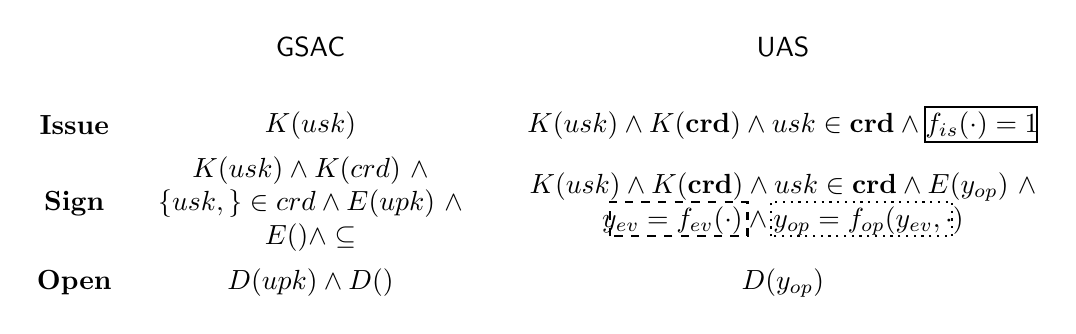
\begin{tikzpicture}

  \pgfdeclarelayer{bg}    % declare background layer
  \pgfsetlayers{bg,main}  % set the order of the layers (main is the standard layer)

  \node (GSAC) at (3.00,3.50) { \GSAC };
  \node (UAS) at (9.00,3.50) { \UAS };

  \node (issue) at (0.00,2.50) { \bf Issue };
  \node (sign) at (0.00,1.50) { \bf Sign };  
  \node (open) at (0.00,0.50) { \bf Open };

  \node (issue-gsac) at (3.00,2.50) { $K(\usk)$ };
  \node[align=center] (sign-gsac) at (3.00,1.50)
  { $K(\usk) \land K(\cred) ~\land$ \\
    $\lbrace \usk,\attrs \rbrace \in \cred \land E(\upk)~\land$ \\
    $E(\attrs) \land \dattrs \subseteq \attrs$ };
  \node (open-gsac) at (3.00,0.50) { $D(\upk) \land D(\attrs)$ };

  \node (issue-uas) at (9.00,2.50)
  { $K(\usk) \land K(\scred) \land \usk \in \scred \land \fissue(\cdot) = 1$ };
  \node[align=center] (sign-uas) at (9.00,1.50)
  { $K(\usk) \land K(\scred) \land \usk \in \scred \land E(\yinsp)~\land$ \\
    $\yeval = \feval(\cdot) \land \yinsp = \finsp(\yeval,\cdot)$
  };
  \node (open-uas) at (9.00,0.50) { $D(\yinsp)$ };

  \draw[draw=black,thick] (10.80,2.29) rectangle ++(1.43,0.44);
  \draw[draw=black,dashed,thick] (6.80,1.09) rectangle ++(1.75,0.44);
  \draw[draw=black,dotted,thick] (8.85,1.09) rectangle ++(2.30,0.44);
    
\end{tikzpicture}

%%% Local Variables:
%%% mode: latex
%%% TeX-master: t
%%% End:

  }
  \caption{Summary of statements proved per operation in \UAS.
    $K(x)$ means proving knowledge of $x$; $E(y)$ means proving correct
    encryption of $y$; $D(z)$ means proving correct decryption of (an encryption
    of) $z$. $\usk \coloneqq$ user secret key; $\scred \coloneqq$ set of
    credentials.}
  \label{fig:proof-blocks-uas}
\end{figure}

From \CUASGen, one can already build known (and more
functionality-limited) schemes from what we call \emph{restrictions} of
\CUASGen simply by giving concrete definitions of \fissue, \feval, and \finsp.
Yet, the model remains the same, and we prove that if such restrictions of
\CUASGen are secure in the \UAS model, they lead to secure constructions for
the related primitives (GS variants, AC variants, etc). To define our generic
construction, we also specify concrete NP relations for the underlying NIZK
proofs for issuing, signing, and opening. These NP relations must not be
considered as immutable, though. Actually, we show how, by making a minor
variation into the one used for signing, a \CUASGen restriction can securely
build ring signatures.

We emphasize that, while -- already before \UAS -- it may have not seemed hard
to build either of these primitives from another, the core of our contribution
is that, with \UAS, one just needs to give concrete definitions of three
functions (or little more). Security of the final primitive then essentially
follows from the fact that it is a secure instantiation of an \UAS scheme. We
believe that this is a powerful notion, that may finally allow research lines
(AC and GS) that have followed different paths to benefit from the findings of
each other. \figref{fig:relations} graphically summarises the relations we prove
between \UAS and other schemes -- although, of course, many more are probably
achievable.

\begin{figure}[ht!]
  \centering
  \scalebox{0.9}{
    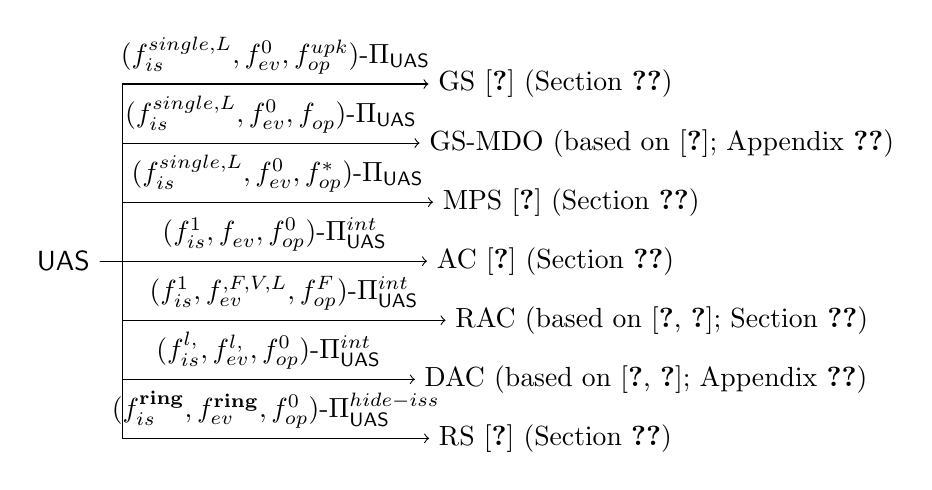
\begin{tikzpicture}

  \node (uas) at (-0.25,2.25) { \bf \UAS };
  
  \node (gs) at (6.00,4.50) { GS \cite{bsz05}
    (\secref{ssec:related-models-gs})};
  \node (gsmdo) at (7.35,3.75) { GS-MDO (based on \cite{seh+12};
    \appref{sapp:related-models-gsmdo}) };
  \node (mps) at (6.20,3.00) { MPS \cite{ngsy22}
    (\secref{ssec:related-models-mps}) };
  \node (ac) at (6.00,2.25) { AC \cite{fhs19}
    (\secref{ssec:related-models-ac}) };
  \node (rac) at (7.35,1.50) { RAC (based on \cite{fhs19,cks10};
    \secref{ssec:related-models-rac}) };
  \node (dac) at (7.15,0.75) { DAC (based on \cite{fhs19,bcc+09};
    \appref{sapp:related-models-dac}) };
  \node (rs) at (6.00,0.00) { RS \cite{bkm06}
    (\secref{ssec:related-models-rs}) };

  \draw[->] (uas) -- (0.50,2.25) -- (0.50,4.50) -- node[midway,above]
  {$(\fissue^{single,L},\feval^0,\finsp^{\upk})$-\CUASGen} (gs);
  \draw[->] (uas) -- (0.50,2.25) -- (0.50,3.75) -- node[midway,above]
  {$(\fissue^{single,L},\feval^0,\finsp^{\smsg})$-\CUASGen} (gsmdo);
  \draw[->] (uas) -- (0.50,2.25) -- (0.50,3.00) -- node[midway,above]
  {$(\fissue^{single,L},\feval^0,\finsp^{\ast})$-\CUASGen} (mps);
  \draw[->] (uas) -- (0.50,2.25) -- node[midway,above]
  {$(\fissue^1,\feval^{\dattrs},\finsp^0)$-$\CUASGen^{int}$} (ac);
  \draw[->] (uas) -- (0.50,2.25) -- (0.50,1.50) -- node[midway,above]
  {$(\fissue^1,\feval^{\dattrs,F,V,L},\finsp^{F})$-$\CUASGen^{int}$} (rac);
  \draw[->] (uas) -- (0.50,2.25) -- (0.50,0.75) -- node[midway,above]
  {$(\fissue^{l,\dattrs},\feval^{l,\dattrs},\finsp^0)$-$\CUASGen^{int}$} (dac);
  \draw[->] (uas) -- (0.50,2.25) -- (0.50,0.00) -- node[midway,above]
  {$(\fissue^{\sring},\feval^{\sring},\finsp^0)$-$\CUASGen^{hide-iss}$} (rs);
    
\end{tikzpicture}

%%% Local Variables:
%%% mode: latex
%%% TeX-master: t
%%% End:

  }
  \caption{Summary of schemes that can be instantiated as restrictions of our
    generic construction, \CUASGen, and proved secure under our \UAS model.
    $\CUASGen^{\ast}$ denotes that minor changes to the basic construction
    beyond the concrete $(\fissue,\feval,\finsp)$-restrictions are needed.
    Between parenthesis we show the adopted reference model, and the section
    offering full detail.
  }
  \label{fig:relations}
\end{figure}

\paragraph{Outline.} %
We give some preliminaries in \secref{sec:preliminaries}. Then proceed with our
\UAS syntax, model, and construction, in \secref{sec:formal-uas}, and show
relationships with other primitives in \secref{sec:relationships}. We conclude
in \secref{sec:conclusion}. Deferred proofs and additional information appear
in the appendices.

%%% Local Variables:
%%% mode: latex
%%% TeX-master: "uas-paper"
%%% End:

\section{Preliminaries}
\label{sec:preliminaries}

% [3 pages max; 1.5 prelim, 1.5 GSAC]

\subsection{Cryptographic Building Blocks}
\label{ssec:cryptobblocks}

Next we introduce the main building blocks we will be using in our
constructions. More detailed definitions and references appear in
\appref{app:crypto-building-blocks}.

\paragraph{Digital Signatures.} %
Defined as a tuple (\SSetup,\SKeyGen,\SSign,\SVerify). Algorithm $\parm \gets
\SSetup(\secpar)$ produces public parameters for the other algorithms.
$(\vk,\sk) \gets \SKeyGen(\parm)$ generates the verification-signing key
pair, algorithm $\sig \gets \SSign(\sk,\msg)$ signs message \msg with
signing key \Ssk, producing signature \Ssig, and $1/0 \gets \SVerify(\vk,
\sig,\msg)$ checks whether \Ssig is a valid signature over \msg, under
verification key \Svk. We rely on existentially unforgeable digital signature
schemes.

\paragraph{Public-Key Encryption.} %
Defined as a tuple (\ESetup,\EKeyGen,\EEnc,\EDec). Algorithm $\parm \gets
\ESetup(\secpar)$ produces public parameters for the other algorithms.
$(\ek,\dk) \gets \EKeyGen(\parm)$ generates the encryption-decryption key
pair, algorithm $\Ec \gets \EEnc(\ek,\msg)$ encrypts message \msg with
encryption key \Eek, producing ciphertext \Ec, and $\msg/\bot \gets \EDec(\dk,
\Ec)$ decrypts ciphertexts using decryption key \Edk. We rely on IND-CCA
public-key encryption schemes.

\paragraph{(Block) Commitment Schemes.} %
Defined as a tuple (\CSetup,\CCommit). Algorithm $\parm \gets
\CSetup(\secpar)$ produces the parameters for committing to values. $\Ccom
\gets \CCommit(\parm, \smsg; r)$ produces a commitment \Ccom over a set of
messages \smsg, using randomness $r$ (which we may omit when explicitly
stating it is not necessary). We will further use commitment schemes that
allow committing to vectors of messages. Therein, the \CCommit algorithm simply
receives a block of messages. In both cases, we require hiding and binding
(block) commitment schemes.

\paragraph{Non-Interactive Zero-Knowledge.} %
We use non-interactive zero-knowledge proofs of knowledge (NIZK), in the CRS
model. Informally, a NIZK scheme over an NP relation \NIZKRel is defined as a
tuple ($\NIZKSetupRel$,$\NIZKProveRel$,$\NIZKVerify^\NIZKRel$).
Algorithm $\NIZKcrs \gets \NIZKSetupRel(\NIZKsecpar)$ produces the common
reference string \NIZKcrs. $\NIZKproof/\bot \gets \NIZKProveRel(\NIZKcrs,
\NIZKx,\NIZKw)$ creates a NIZK proof of knowledge of witness \NIZKw for \NIZKx
such that $(\NIZKw,\NIZKx) \in \NIZKRel$. $1/0 \gets \NIZKVerifyRel
(\NIZKcrs,\NIZKx,\NIZKproof)$ verifies the proof. Within NIZK systems, we
further need schemes that provide simulation-extractability, which in a nutshell
means that no adversary can produce a proof from which we cannot extract a
witness, even after seeing polynomially many simulated proofs. To model
simulation-extractable NIZKs, we further need algorithms \NIZKSimSetup,
\NIZKSim, and \NIZKExtract, that allow simulating proofs and extracting
witnesses. The properties we build on are completeness, soundness,
zero-knowledgeness, and simulation-extractability.

\paragraph{Signatures over Blocks of Committed Messages, with proofs.} %
We use signature schemes that allow signing blocks of messages, or commitments
to blocks of messages, and which are furthermore compatible with (efficient)
proof systems over the produced signature and signed (commitments to) messages.
For this purpose, we define such schemes as a tuple (\SBCMSetup,\SBCMKeyGen,
\SBCMCom,\SBCMSign,\SBCMVerify). Algorithm $\parm \gets \SBCMSetup(\secpar)$
produces the public parameters for the scheme. %
$(\vk,\sk) \gets \SBCMKeyGen(\parm)$ produces a verification-signing
key pair. $\sig/\bot \gets\langle \SBCMCom(\vk,\overline{\smsg},\smsg),
  \SBCMSign(\sk,\smsg) \rangle$ is an interactive protocol between a user, who
runs \SBCMCom and has a set of messages $\overline{\smsg}$ to be block-committed,
and a signer, who owns signing key \sk; both also receive common input a
block of messages \smsg. The output of the protocol is a signature over
$\overline{\smsg} \cup \smsg$. Algorithm $1/0 \gets \SBCMVerify(\vk,
\sig,\overline{\smsg},\smsg)$ verifies a signature \sig over message set
$\overline{\smsg} \cup \smsg$. In addition, the
produced signatures must be compatible with (efficient) NIZK proofs of knowledge
of a signature, and of (arbitrary) claims over the signed (committed) messages.
An \SBCM scheme must provide one-more-forgery type of security.

\subsection{Notation}
\label{ssec:notation}

We follow common notation habits. $y \gets A(x)$ means that algorithm $A$, on
input $x$, produces output $y$. When $A$ is a probabilistic process, and we want
to make explicit the randomness $r$, we use $y \gets A(x;r)$. $\langle y_A,y_B
\rangle \gets \langle A(x_A),B(x_B)\rangle$ denotes algorithms $A$ and $B$,
running an interactive protocol, where $A$ receives $x_A$ as input and produces
$y_A$ as output, and $B$ receives $x_B$ and produces $y_B$.
%
Our generic constructions rely on the previously defined building blocks, which
share common (but different)
tokens: e.g., we will resort to several NIZK proofs instances. To distinguish
them, we may use subscripts or superscripts: e.g., $\NIZKRel_A$ denotes the
NP relation used within some algorithm $A$, $\NIZKSetupRel$ means that
the setup algorithm of an underlying NIZK system is performed associated to
relation $\NIZKRel$; $\SBCMparm$ are the public parameters for an \SBCM scheme,
and $\Eparm$ are the public parameters for an encryption scheme. Variables
written in bold font denote sets, e.g., while we use \ipk to denote a single
issuer public key, \sipk denotes a set of issuer's public keys. To refer to
a specific element of a set, we use subindexes, e.g., $\sipk_i$ is the $i$-th
\ipk within \sipk.
%
We also assume the existence of a well defined attribute space over which
issuers in our schemes can issue credentials on. We denote this set with
\AttrSpace.

%%% Local Variables:
%%% mode: latex
%%% TeX-master: "uas-paper"
%%% End:

\section{Formalising \UAS}
\label{sec:formal-uas}

% [11 pages max]

Next we formalise our notion of Universal Anonymous Signatures
(\UAS). We define its syntax, model, and give a generic construction, which
we prove secure. 

The main contribution of this section is giving a simple syntax and model that
still allow spanning a wide variety of related schemes. This is in part
achieved by combining aspects of GS and AC schemes. Yet, the main tool for
generalisation are three functional placeholders, governing the conditions to be
checked during issuance, the information to be revealed alongside signatures,
and extractable from them. However, at the modelling level we are not concerned
with the ``code'' of these functions, but only with the correctness of their
computation, and with capturing security and privacy despite introducing
configurable functions.

% \paragraph{Users and credentials.} %
% In our model, every single user may have multiple credentials. In this
% setting, a perhaps too strict assumption we make is that, once a user gets
% compromised, all of the credentials owned by that user are compromised too.
% While there may be real world situations for which this is too aggressive, it is
% certainly a worst-case scenario, and greatly simplifies the modelling.
% %
% % Somehow related, we model a scheme in which users generate their secret keys in
% % a standalone way, and then leverage these keys to request credentials. This may
% % seem too ideal as a model for real world situations, as we cannot know how
% % many keys a user has generated. However, we argue that this can in fact be very
% % close to reality, where a well-known issuer, after properly identifying a user,
% % attests the (possibly blinded) public key this user proves control of. Indeed,
% % our model and syntax support exactly this approach, by allowing users to
% % leverage previously obtained credentials in order to request new ones.
% % A consequence of this is that, if ``one user'' generates (e.g.) two keys, and
% % then uses each of these keys to request multiple credentials, then from the
% % point of view of our modelling, we see this \emph{cryptographically} as two
% % different users -- and, anyway, that same ``user'' cannot combine credentials
% % bound to different keys.

% \paragraph{Users and issuers.} %
% A relevant aspect of our model is that users and issuers are basically the
% same: an entity with a key pair. The difference is that, when users wish to
% become issuers, they advertise their public keys, along with their conditions
% for granting credentials. To simplify, we just assume that they somehow
% ``publish their public keys'', which can be done in several ways in practice.

\subsection{Syntax}
\label{ssec:syntax-uas}

Users generate their key pair, and then optionally advertise
their public key and conditions for issuance in order to become issuers. When
openers generate their key pairs, they include the function they will apply to
anonymous signatures. Users can later leverage (one or more of) their
credentials to request new ones, or to produce an anonymous signature. Issuance
only succeeds if the user's credentials (if any) meet the issuer's requirements.
Signatures may directly output some information derived from the user's data.
Also, each signature has a selected opener (probably, by the user and/or
verifier), who can later \emph{extract only the information that is defined by
  the chosen opener's key}. When openers extract their information, they also
prove the correctness of the result.

In detail, an \UAS scheme is composed by the following algorithms:

\begin{description}
\item[$\Setup(\secpar) \rightarrow \parm$.] Given a security parameter \secpar,
  returns a global system parameter variable \parm. We assume that \parm are
  available to all other functions.
\item[$\KeyGen(\parm) \rightarrow (% \Ccom,r,
  \upk,\usk)$.] Given \parm, a user
  runs \KeyGen to generate its user key pair% , and a commitment \Ccom to the
  % public key, with randomness $r$
  . 
\item[$\OKeyGen(\parm,\finsp) \rightarrow (\opk,\osk)$.] Given \parm, and
  function \finsp, an opener runs \OKeyGen to generate its key pair. \finsp
  defines the utility extractable from signatures.
\item[$\ISet(\upk,\usk,\fissue) \rightarrow \ipk$.] Given a user key
  pair, and an issuance function \fissue for checking that credential requesters
  meet some conditions to be issued a credential, an existing user runs \ISet to
  extend the user public key, enabling this user to issue credentials meeting
  \fissue.
%\item[$\UKeyGen(\parm) \rightarrow (\upk,\usk)$.] Given \parm, returns a user's
%  key pair.
\item[$\langle
  \Obtain(\usk,\ipk,\sCred,\attrs),
  \Issue(\isk,\sipk,\attrs))  
  \rangle \rightarrow \langle \Cred/\bot,R/\bot
  \rangle$.] %
  This interactive protocol lets a user with key \usk receive a credential
  $\Cred=(\cid,\attrs,\cred,\ipk)$
  from an issuer in the system. $\cid=(\cidi,\cidu)$ is a unique identifier for
  the credential, where issuer and user randomly pick \cidi and \cidu,
  respectively (to ease notation, whenever we write just \cid, we mean $(\cidi,
  \cidu)$). \ipk is the issuer's public key and \cred is the actual credential,
  on attribute set \attrs. The user may leverage a set of previously obtained
  credentials $\sCred=\lbrace (\cid_i=(\cidi_i,\cidu_i),\cattrs_i,\cred_i,
  \ipk_i)\rbrace_{i\in[n]}$, from which we may omit the $\ipk_i$s for
  readability. The user outputs the produced credential \Cred, while the issuer
  outputs $R \gets (\yissue,\utrans)$, for some value $\yissue$ output by
  the \fissue function defined by the issuer, and $\utrans=(U,I)$ being the
  transcript of the communication% , where $U$ contains the messages sent by
  % the user, and $I$ those sent by the issuer
  .
\item[$\Sign(\usk,\opk,\sCred,\msg,\feval) \rightarrow (\sig,\yeval)$.] %
  Upon receiving user secret key \usk, opener public key \opk, 
  credentials \sCred, message \msg and evaluation function \feval, returns
  signature \sig, and a value \yeval. We use use \Sig to denote the
  tuple $(\sig,\yeval)$.
\item[$\Verify(\opk,\sipk,\Sig,\msg,\feval) \rightarrow 1/0$.]
  Checks whether $\Sig = (\sig,\yeval)$ is a valid signature
  over message \msg, from a user with credentials issued by issuers with public
  keys in \sipk, for evaluation function \feval and opener key \opk.
\item[$\Open(\osk,\sipk,\Sig,\msg,\feval) \rightarrow
  (\yinsp,\iproof)/\bot$.]
  Run by the opener with private key \osk. Receives a signature $\Sig=
  (\sig,\yeval)$ over message \msg and evaluation function \feval,
  generated using credentials by issuers with public keys in \sipk.
  If \Sig is valid, the function outputs a value $\yinsp$, and a proof of
  correct opening \iproof.
\item[$\Judge(\opk,\sipk,\yinsp,\iproof,\Sig,\msg,\feval) \rightarrow 1/0$.] %
  Checks if \iproof is a valid opening correctness proof for the value \yinsp,
  obtained by applying \Open to the the signature $\Sig = (\sig,\yeval)$
  over message \msg, and for evaluation function \feval. 
\end{description}

\paragraph{Issuance, evaluation, and opening functions.} %
These are the functional placeholders that allow modulating the behaviour of the
resulting instantiation. They control the conditions for issuing new
credentials, the information revealed alongside signatures, or extractable
from them. In all cases, the user computes them, and proves correctness of
such computation. We give concrete examples in \secref{sec:relationships}.

\begin{description}
\item[$\fissue: (\upk,\cid,\attrs,\lbrace (\cid_i,\cattrs_i)\rbrace_{i \in [n]})
  \rightarrow \yissue$.] Chosen
  by each issuer within a family of functions \famfissue, the issuance function
  defines the conditions required by the issuer to grant a credential
  with identifier $\cid = (\cidi,\cidu)$, over attributes \attrs, when requested
  by a user with public key \upk, leveraging a set of $n$ previously obtained
  credentials with identifiers and attributes given by $\lbrace (\cid_i,
  \cattrs_i) \rbrace_{i \in [n]}$ (where $n$ may be $0$). \fissue returns
  a value $\yissue \in \rngfissue \cup \lbrace 0 \rbrace$, where we adopt the
  convention that $\yissue = 0$ means that the issuance request is denied; and
  $\yissue \neq 0$ means that the request is approved. \fissue functions must be
  \UAS-acceptable, as defined in \defref{def:uas-acc-func}.
\item[$\feval: (\upk,\lbrace(\cid_i,\cattrs_i)\rbrace_{i \in [n]},\msg)
  \rightarrow (\yeval^0,\yeval^1)$.] Signing evaluation functions (or, simply,
  evaluation functions), from a
  family of functions \famfeval, can be set on a per-signature basis. They
  receive the user public key \upk, a set of credentials with identifiers
  and attributes $\lbrace (\cid_i,\cattrs_i) \rbrace_{i \in [n]}$
  (where $n \ge 1$), and the message to be signed \msg. \feval outputs two
  values, $\yeval^0$ and $\yeval^1$. Both must belong in a well defined set
  \rngfeval. For readability, we write $\Yeval = (\yeval^0,\yeval^1)$.
\item[$\finsp: (\Yeval,\upk,\lbrace (\cid_i,\cattrs_i) \rbrace_{i \in [n]},
  \msg) \rightarrow \yinsp$.]
  Chosen by openers from a family of functions \famfinsp. The opening
  functions define what utility value (derived from the user's secret key,
  credentials' identifiers and attributes used for signing, and signed message)
  should be extractable by an opener. Its behaviour can be modulated by \Yeval,
  and it outputs a value \yinsp, which must belong in a well defined set
  \rngfinsp.
\end{description}

Concerning \fissue functions, our \UAS model requires them to be
\UAS-acceptable. At a high level, this requires that, conditioned on \fissue
functions accepting the request (i.e., returning a non-zero value), they do not
reveal anything about the signer's data used as input. This is formally captured
in \figref{fig:uas-acceptable}.
%
A \UAS construction thus can only be secure if the \fissue functions it uses
are \UAS-acceptable.

\begin{figure}[ht!]
  \centering  
  \scalebox{0.85}{
    \procedure[linenumbering=on]{$\Exp^{\UAS-acc-b}_\adv(1^\secpar)$}{%
      \parm \gets \Setup(1^\secpar) \\
      (\upk,\usk) \gets \KeyGen(\parm) \\
      (\st,\attrs, \lbrace (\cidi,\cidu,\cattrs_i) \rbrace_{i\in[n]})
      \gets \adv(\upk) \\
      y \gets \fissue(\upk,\cid,\attrs,\lbrace (\cid_i,\cattrs_i)
      \rbrace_{i\in[n]}) \\
      \pcif y = 0: \pcreturn \bot \\
      \pcif b=0: \yissue^* \gets y;~
      \pcelse:~\yissue^* \getr \rngfissue \setminus \lbrace 0 \rbrace \\
      b^* \gets \adv(\st,\yissue^*) \\
      \pcreturn b^*
    }
  }
  \label{fig:uas-acceptable}
  \caption{Formal definition of \UAS-acceptable \fissue functions.}
\end{figure}

\begin{definition}{(\UAS-acceptable \fissue functions)}
  \label{def:uas-acc-func}
  A \fissue function is \UAS-acceptable if, for any p.p.t. adversary \adv,
  $|\Pr[\Exp^{\UAS-acc-1}_\adv(1^\secpar)=1]-\Pr[\Exp^{\UAS-acc-0}_\adv
  (1^\secpar)=0]|$ is a negligible function of $1^\secpar$.
\end{definition}

Next, we define the concept of \CUASGen restrictions. These are special
cases of our generic construction that target a concrete variant of the
utility-privacy trade-off by defining concrete \fissue, \feval and \finsp
functions. Security of \CUASGen implies security of its restrictions, if
the chosen \fissue function is \CUASGen-acceptable.

\begin{definition}{(\CUASGen restrictions)}
  \label{def:uas-restrictions}
  Let \CUASGen be a construction of an \UAS scheme, secure according to
  the model defined in \secref{ssec:model-uas}, and three functions $\fissue^a$,
  $\feval^b$, $\finsp^c$ compatible with the previous definitions. We say that
  \CUASGen, instantiated with $\fissue^a$, $\feval^b$, and $\finsp^c$, is a
  $(\fissue^a,\feval^b,\finsp^c)$-restriction of \CUASGen.
\end{definition}

\subsection{Security Model}
\label{ssec:model-uas}

We define the security expected from an \UAS scheme using a game-based approach.
An \UAS scheme must ensure privacy at credential issuance, meaning that two
runs of the credential issuance protocol should not leak any information beyond
necessary about the user requesting the credential. Note that this is now
crucial for privacy since \UAS allows multiple credentials per
user -- thus, knowing what user is requesting which credential can lead to user
profiling. It must also ensure signature privacy, meaning that no information
can be learned by third parties from a signature, beyond what the user chooses
to reveal, and what may be extractable by the chosen opener. Unforgeability
requires that \UAS schemes ensure that the claims used to support a credential
request cannot be falsified, and that no adversary is able to falsify the
correctness proofs for the claims included in the signatures. In addition, we
require all credentials involved in the corresponding process to be associated
to the same, and known, user key. Finally, \UAS schemes inherit the useful
non-frameability property of GS schemes where even the issuer is corrupt. In
this case, we can ensure that no honest user can be framed with having created a
signature that s/he did not create -- although the concept may get a bit
blurred, as there is no traditional opening.
%
We describe next the global variables and oracles that we use in our modelling.

\paragraph{Global Variables.} %
Users are referred to with user identifiers, \uid; for credentials, we use \cid;
and for openers, \oid. Although issuers are ``extended'' users, and thus can be
identified by their \uid, we mostly use \iid to refer to a user acting as
issuer, especially for clarity in operations involving both a user and an
issuer.
%
For notational convenience, we often use these identifiers instead of the
corresponding user/issuer/opener keys.
%
All tables/sets are initialised as empty tables/sets. We use the following sets
and tables in our definitions:

\begin{description}
\item[$\mathsf{H}\lbrace\mathsf{U},\mathsf{I},\mathsf{O} \rbrace$.] Sets of
  honest {\uid}s/{\iid}s/{\oid}s.
\item[$\mathsf{C}\lbrace\mathsf{U},\mathsf{I},\mathsf{O} \rbrace$.] Sets of
  corrupt {\uid}s/{\iid}s/{\oid}s.
\item[\UK,\IK,\OK.] Tables storing key pairs of users $(\upk,\usk)$, issuers
  $(\ipk,\isk)$, and openers $(\opk,\osk)$, indexable by \uid, \iid, and \oid,
  respectively. Issuers' public keys contain a \fissue function, and
  openers' public keys contain a \finsp function.
\item[\PUBUK,\PUBIK,\PUBOK and \PRVUK,\PRVIK,\PRVOK.] Shorthands referring to
  public keys of users, issuers or openers ($\mathsf{PXK}$) or their private
  keys ($\mathsf{SXK}$).
\item[\CRED.] Indexable by \cid, it stores
  tuples of the form $(\uid,\cred,\iid,\attrs,n,\lbrace (\cid_i,\iid_i)
  \rbrace_{i \in [n]})$, where \uid is the identifier of the owner of the
  credential, \cred (when available) is the credential itself, \iid is the
  identifier of the credential issuer, \attrs are the attributes included in
  \cred, $n$ is the number of credentials used to support this request, and
  $(\cid_i,\iid_i)$ for $i \in [n]$ are the corresponding credential and issuer
  identifiers. For notational convenience, we may use $\CRED[\scid]$
  to refer to $\CRED[\cid]$ for all {\cid}s in a set \scid. Also, when clear
  from context, we sometimes use $\CRED[\cid]$ (resp. $\CRED[\scid]$) to
  mean \cred (resp. \scred) in $\CRED[\cid] = (\cdot,\cred,\cdot,\cdot,
  \cdot,\cdot)$ (resp. $\CRED[\scid]$).
\item[\CCRED.] Like \CRED, but tracks challenge credentials.
\item[\OWNR.] When we write $\OWNR[\cid]$ we mean
  ``\uid such that $\CRED[\cid] = (\uid,\cdot,\cdot,\cdot,\cdot,\cdot)$'', or
  $\bot$ if there is no such \uid. We also use \OWNR over a set of {\cid}s
  (\scid). In that case, $\OWNR[\scid]$ returns $\bot$ if
  not all passed {\cid}s belong to the same \uid. Since $\bot$ is not a valid
  \uid, all conditions checking membership of the output of \OWNR to a list of
  users equal false if \OWNR returns $\bot$.
\item[\ATTR.] When we write $\ATTR[\cid]$ we mean
  ``\attrs such that $\CRED[\cid] = (\cdot,\cdot,\cdot,\attrs,\cdot,\cdot)$''.
\item[\ISR.] When we write $\ISR[\cid]$ we mean
  ``\iid such that $\CRED[\cid] = (\cdot,\cdot,\iid,\cdot,\cdot,\cdot)$''.
\item[\SIG.] Maintains signatures generated via the \SIGN oracle. Entries of
  this table are $(\oid,\scid,\sig,\Yeval,\msg,\feval)$ tuples, where \oid is
  the opener, \scid is the set of identifiers of the credentials used for
  signing, \feval is the signing evaluation function, and \sig and \msg are the
  produced signature and signed message.
\item[\CSIG.] Stores challenge signatures output to the adversary in the
  signature anonymity game, and is indexable by challenge signatures \csig.
  Each entry contains also $\cuid_b$ and $\cscid_b$, respectively the challenge
  user  and credential identifiers set used to produce \csig; as well as the
  corresponding challenge user and credential set indexed by the complementary
  $1-b$; the signed message \msg and signing evaluation function \feval, the
  result of \feval, \Yeval, and the opener identifier \oid.
\end{description}

\paragraph{Oracles.} %
We leverage the following oracles, formalised in \figref{fig:oracles1} and
\figref{fig:oracles2}.

\begin{description}
% \item[\IGEN.] Adds a new issuer to the game, generating its keypair and setting
%   the associated issuance function.
\item[\HUGEN.] Adds a new honest user, generating its key pair.
\item[\CUGEN.] Adds a new corrupt user. Sets its \upk to the
  one given by the adversary.  
\item[\OGEN.] Adds a new opener, generates its key pair and sets its opening
  function.
% \item[\ICORR.] Corrupts an existing (and honest) issuer, by giving its secret
%   key to the adversary.
\item[\ISET.] ``Upgrades'' a user to become an issuer, specifying its
  \fissue function.
\item[\UCORR.] Corrupts an existing honest user, giving its \usk to the
  adversary. If the user was also an issuer, it becomes a corrupt issuer too.
\item[\OCORR.] Corrupts an existing honest opener, giving its \osk to the
  adversary.
% \item[\HUGEN.] Adds a new honest user to the game, by honestly generating
%   the user's key pair.
% \item[\CUGEN.] Adds a new corrupt user to the game or, if the specified
%   user already exists and is honest, corrupts it, leaking its key and
%   credentials.
\item[\RREG.] Reads the given transcript table entry.
\item[\WREG.] Sets a transcript table entry to the given value.
\item[\OBTISS.] Lets the adversary add a new honestly generated credential to
  the game, on behalf of an honest user.
\item[\OBTAIN.] Enables the adversary to play the role of a dishonest issuer, by
  letting it interact with honest users who want to receive credentials.
\item[\ISSUE.] Allows the adversary to play the role of dishonest users,
  requesting an honest issuer to produce credentials for them.
\item[\SIGN.] Lets the adversary get signatures using credentials from honest
  users.
\item[\OPEN.] Given an honestly produced signature, outputs the result of the
  opening function, along with a correctness proof.
\item[\OBTCHALb.] Upon receiving a target credential identifier, two challenge
  users and credential sets, an honest issuer identifier, and a set of
  attributes, issues a credential for the challenge user and credential set
  defined by the bit $b$. 
\item[\CHALb.] Upon receiving two challenge users and credential sets, a common
  singing evaluation function and a message, returns a signature produced by one
  of these two user and credential sets, defined by the bit $b$.
\end{description}

{%\setlength\intextsep{\sep}
  \begin{figure*}[ht!]
    \centering
    \scalebox{0.85}{

      \begin{minipage}[t]{0.55\textwidth}

        % \procedure{$\IGEN(\iid,\fissue)$}{%
        %   \pcif \iid \in \HI \lor \iid \in \CI: \pcreturn \bot \\
        %   \pcif \fissue \notin \famfissue: \pcreturn \bot \\
        %   (\ipk,\isk) \gets \IKeyGen(\parm) \\
        %   \IK[\iid] \gets ((\ipk,\fissue),\isk) \\
        %   \HI \gets \HI \cup \lbrace \iid \rbrace \\
        %   \pcreturn \ipk \\
        % }

        % \procedure{$\ICORR(\iid)$}{%
        %   \pcif \iid \in \CI \lor \iid \notin \HI: \pcreturn \bot \\
        %   \HI \gets \HI \setminus \lbrace \iid \rbrace \\
        %   \CI \gets \CI \cup \lbrace \iid \rbrace \\
        %   \pcreturn \isk \\
        % }        

        % \procedure{$\HUGEN(\uid)$}{%
        %   \pcif \uid \in \HU \lor \uid \in \CU: \pcreturn \bot \\
        %   (\upk,\usk) \gets \UKeyGen(\parm) \\
        %   \UK[\uid] \gets (\upk,\usk);
        %   \HU \gets \HU \cup \lbrace  \uid \rbrace \\
        %   \pcreturn \top \\
        % }

        \procedure{$\HUGEN(\uid)$}{%
          \pcif \uid \in \HU \lor \uid \in \CU: \pcreturn \bot \\
          (\upk,\usk) \gets \KeyGen(\parm) \\
          \UK[\uid] \gets (\upk,\usk) \\
          \HU \gets \HU \cup \lbrace \uid \rbrace \\
          \pcreturn \upk \\
        }
        
        \procedure{$\UCORR(\uid)$}{%
          \pcif \uid \in \CU \lor \uid \notin \HU: \pcreturn \bot \\
          \pcif \uid \in \HI \cup \CI: \pcreturn \bot \\
          \HU \gets \HU \setminus \lbrace \uid \rbrace \\
          \CU \gets \CU \cup \lbrace \uid \rbrace \\
          \pcreturn (\PRVUK[\uid],\CRED[\uid]) \\
        }
        
        \procedure{$\ICORR(\uid)$}{%
          \pcif \uid \notin \HI: \pcreturn \bot \\
          \HI \gets \HI \setminus \lbrace \uid \rbrace \\
          \CI \gets \CI \cup \lbrace \uid \rbrace \\
          \pcreturn(\PRVUK[\uid],\CRED[\uid]) \\
        }

        \procedure{$\OGEN(\oid,\finsp)$}{%
          \pcif \oid \in \HO \lor \oid \in \CO: \pcreturn \bot \\
          \pcif \finsp \notin \famfinsp: \pcreturn \bot \\
          (\opk,\osk) \gets \OKeyGen(\parm) \\
          \OK[\oid] \gets ((\opk,\finsp),\osk) \\
          \HO \gets \HO \cup \lbrace \oid \rbrace \\
          \pcreturn \opk
        }
        
      \end{minipage}
    }
    \scalebox{0.85}{
      
      \begin{minipage}[t]{.5\textwidth}

        \procedure{$\CUGEN(\uid,\upk)$}{%          
          \pcif \uid \in \HU \lor \CU: \pcreturn \bot \\
          \CU \gets \CU \cup \lbrace \uid \rbrace \\          
          \UK[\uid] = (\upk,\bot) \\          
          \pcreturn \top \\
        }

        \procedure{$\ISET(\uid,\fissue)$}{%
          \pcif \uid \notin \HU \cup \CU: \pcreturn \bot \\
          \pcif \uid \in \HI \cup \CI: \pcreturn \bot \\
          \pcif \fissue \notin \famfissue: \pcreturn \bot \\
          \ipk \gets \ISet(\PUBUK[\uid],\PRVUK[\uid],\fissue) \\
          \IK[\uid] \gets ((\ipk,\fissue),\PRVUK[\uid]) \\
          \pcif \uid \in \HU: \HI \gets \HI \cup \lbrace \uid \rbrace \\
          \pcif \uid \in \CU: \CI \gets \CI \cup \lbrace \uid \rbrace \\
          \pcreturn \ipk \\
        }        
        
        \procedure{$\OCORR(\oid)$}{%
          \pcif \oid \in \CO \lor \oid \notin \HO: \pcreturn \bot \\
          \pcif \exists (\oid,\cdot,\cdot,\cdot,\cdot,
          \cdot,\cdot,\cdot,\cdot) \in \CSIG: \pcreturn \bot \\
          \HO \gets \HO \setminus \lbrace \oid \rbrace \\
          \CO \gets \CO \cup \lbrace \oid \rbrace \\
          \pcreturn \osk \\
        }

        \procedure{$\RREG(i)$}{%
          \pcreturn \trans[i] \\
        }                

        \procedure{$\WREG(i,\rho)$}{%
          \trans[i] \gets \rho
        }        
        
      \end{minipage}
      
    }

    \caption{Detailed oracles available in our model (1/2). Oracles for
      key generation.}
    \label{fig:oracles1}
  \end{figure*}
}

{%\setlength\intextsep{\sep}
  \begin{figure*}[htp!]
    \centering
    \scalebox{0.85}{
      \hspace*{-2em}
      \begin{minipage}[t]{0.58\textwidth}

        \procedure{$\OBTISS(\uid,\iid,\attrs,\lbrace (\cid_i,\iid_i)
          \rbrace_{i \in [n]})$}{%
          \pcif \uid \notin \HU \lor \iid \notin \HI: \pcreturn \bot \\
          \pcif \exists i \in [n]~\suchthat~\cid_i \in \CCRED: \pcreturn \bot \\
          \langle \Cred, R \rangle \gets
          \langle \Obtain(\UK[\uid]\CRED[\lbrace \cid_i\rbrace_{i\in[n]}],\attrs), \\
          \hspace*{50pt} \Issue(\PRVIK[\iid],\ISR[\lbrace \cid_i\rbrace_{i\in[n]}],\attrs)
          \rangle \\
          (\cid = (\cidi,\cidu),\cdot,\cdot,\cdot) \gets \Cred \\
          \pcif \CRED[\cid] \neq \bot \lor \CCRED[\cid] \neq \bot:
          \pcreturn \bot \\
          \trans[\cid] \gets R \\
          \CRED[\cid] \gets (\uid, \cred, \iid, \attrs, n,
          \lbrace(\cid_i,\iid_i)\rbrace_{i\in[n]}) \\
          \pcreturn \top \\
        }

        \procedure{$\ISSUE(\uid,\iid,\attrs,\siid=
          \lbrace \iid_i\rbrace_{i\in[n]})$}{%
          \pcif \uid \notin \CU \lor \iid \notin \HI: \pcreturn \bot \\
          \langle \cdot, R \rangle \gets
          \langle \adv, 
          \Issue(\PRVIK[\iid],\siid,\attrs) \rangle \\
          (\cdot,\cdot,\cid=(\cidi,\cdot)) \gets R \\
          \pcif \CRED[(\cidi,\cdot)] \neq \bot \lor \CCRED[(\cidi,\cdot)]
          \neq \bot: \\
          \pcind \pcreturn \bot \\          
          \trans[\cid] \gets R \\
          \CRED[\cid] \gets (\uid,\cdot,\iid,\attrs,n,\lbrace(\cid_i,
          \iid_i)
          \rbrace_{i\in[n]}) \\
          \pcreturn \top \\          
        }

        \procedure{$\SIGN(\oid,\scid=\lbrace\cid_i\rbrace_{i\in[n]},\msg,
          \feval)$}{%
          \uid \gets \OWNR[\scid] \\
          \pcif \uid \notin \HU \lor \feval \notin \famfeval: \pcreturn \bot \\
          \pcif \exists i \neq j \in [n]~\suchthat~\cid_i \in \CRED \land
          \cid_j \in \CCRED: \\
          \pcind \pcreturn \bot \\
          \Sig \gets \Sign(\UK[\uid],\PUBOK[\oid],\scid,\msg,\feval) \\
          \Yeval=(\yeval^0,\yeval^1) \gets \feval(\PUBUK[\uid],\scid,\msg) \\
          \SIG[\uid] \gets \SIG[\uid] \cup
          \lbrace (\oid,\scid,\Sig,\Yeval,\msg,\feval) \rbrace \\
          \pcreturn \Sig \\
        }        

        \procedure{$\OPEN(\oid,\Sig,\msg)$}{%
          \textrm{Let}~\uid~\textrm{be s.t.}~(\cdot,\scid,\Sig,\Yeval,\cdot,
          \feval)
          \in \SIG[\uid] \\
          (\yinsp,\iproof) \gets
          \Open(\PRVOK[\oid],\PUBIK[\scid],\Sig,\msg,\feval) \\
          \pcif \CSIG[\Sig] \neq \bot: \\
          \pcind \textrm{Parse $\CSIG[\Sig]$ as $(\oid,\cuid_b,\scid_b,
            \Yeval,\msg,\feval$} \\          
          \hspace*{83pt}\cuid_{1-b},\cSig_{1-b},\scid_{1-b},
          \TYeval) \\
          \pcind (\tyinsp,\tiproof) \gets
          \Open(\PRVOK[\oid],\PUBIK[\scid],\\
          \hspace*{107pt} \cSig_{1-b},\msg,\feval) \\
          \pcind \pcif \tyinsp \neq \yinsp: \pcreturn \bot \\
          \pcreturn (\yinsp,\iproof)
        }
        
      \end{minipage}
    }
    \scalebox{0.85}{
      
      \begin{minipage}[t]{.55\textwidth}

        \procedure{$\OBTAIN(\uid,\iid,\attrs,\lbrace (\cid_i,\iid_i)
          \rbrace_{i\in[n]})$}{%
          \pcif \uid \notin \HU \lor \iid \notin \CI: \pcreturn \bot \\
          \pcif \exists i \in [n]~\suchthat~\cid_i \in \CCRED: \pcreturn \bot \\
          \pcind \pcreturn \bot \\
          \langle \Cred, \cdot \rangle \gets
          \langle \Obtain(\UK[\uid],\PUBIK[\iid],\lbrace \cid_i\rbrace_{[n]},
          \attrs),\adv \rangle \\
          (\cid = (\cdot,\cidu), \cdot,\cdot,\cdot) \gets \Cred \\
          \pcif \CRED[(\cdot,\cidu)] \neq \bot \lor \CCRED[(\cidu,\cdot)] \neq
          \bot: \pcreturn \bot \\          
          \CRED[\cid] \gets (\uid,\cred,\iid,\attrs,n,\lbrace(\cid_i,
          \iid_i) \rbrace_{i\in[n]}) \\
          \pcreturn \top
        }

        \procedure{$\OBTCHALb(\cuid_{0,1},\iid,\attrs,
          \stackrel{\cscid_{\lbrace 0,1 \rbrace}}
          {\lbrace(\pcbox{(\ccid_{0,i},\ccid_{1,i})}},\iid_i)\rbrace_{i\in[n]})$}{%
          \pcif \cuid_0 \notin \HU \lor \cuid_1 \notin \HU: \pcreturn \bot \\
          \pcif \iid \notin \CI: \pcreturn \bot \\
          \pcif \exists i\in[n]~\suchthat~
          \PUBIK[\cscid_{0,i}] \neq \PUBIK[\cscid_{1,i}]: \pcreturn \bot \\
          \pcif \pcfor d \in \bin,~ \exists \cid' \in \cscid_d~\suchthat~\cid'
          \in \CRED: \\
          \pcind \pcreturn \bot \\          
          \langle \Cred, \cdot \rangle \gets
          \langle \Obtain(\PRVUK[\cuid_b],\PUBIK[\iid],\cscid_b,\attrs),
          \adv \rangle \\
          (\cid = (\cidi,\cidu),\cdot,\cdot,\cdot) \gets \Cred \\
          \textrm{Parse}~\PUBIK[\iid]~\textrm{as}~((\cdot,\fissue),\cdot) \\
          \pcif 0(\fissue(\PUBUK[\cuid_0],\cid,\attrs,\lbrace
          (\ccid_{0,i},\ATTR[\ccid_{0,i}])\rbrace_{i\in[n]})) \neq \\
          \pcind 0(\fissue(\PUBUK[\cuid_1],\cid,\attrs,\lbrace
          (\ccid_{1,i},\ATTR[\ccid_{1,i}])\rbrace_{i\in[n]})): \\
          \pcind \pcreturn \bot \\          
          \pcif \CRED[(\cdot,\cidu)] \neq \bot \lor
          \CCRED[(\cdot,\cidu)] \neq \bot: \pcreturn \bot \\          
          \CCRED[\cid] \gets (\cuid_b,\cred,\iid,\attrs, n,
          \lbrace(\ccid_{b,i},\iid_i)\rbrace_{i\in[n]}) \\
          \pcreturn \top
        }

        \procedure{$\CHALb(\oid,\stackrel{\cscid_{\lbrace 0,1 \rbrace}}{\pcbox{
            \lbrace (\ccid_{0,i},\ccid_{1,i})
            \rbrace_{i\in[n]}}},\msg,\feval)$}{%
          \pcfor d\in\bin: \cuid_d \gets \OWNR[\cscid_d] \\
          \pcif \cuid_0 \notin \HU \lor \cuid_1 \notin \HU: \pcreturn \bot \\
          \pcif \exists i\in[n]~\suchthat~
          \PUBIK[\cscid_{0,i}] \neq \PUBIK[\cscid_{1,i}]: \\
          \pcind \pcreturn \bot \\
          \pcif \feval \notin \famfeval: \pcreturn \bot \\
          \Yeval = (\yeval^0,\yeval^1) \gets \feval(\PUBUK[\cuid_0],\cscid_0,
          \msg) \\
          \TYeval = (\tyeval^0,\tyeval^1) \gets
          \feval(\PUBUK[\cuid_1],\cscid_1,\msg) \\
          \pcif \yeval^0 \neq \tyeval^0: \pcreturn \bot \\   
          \cSig_b \gets \Sign(\PRVUK[\cuid_b],\PUBOK[\oid],\cscid_b,\msg,
          \feval) \\
          \cSig_{1-b} \gets \Sign(\PRVUK[\cuid_{1-b}],\PUBOK[\oid],\cscid_{1-b},
          \msg,\feval) \\          
          \CSIG[\cSig_b] \gets 
          \lbrace (\oid,\cuid_b,\cscid_b,\Yeval,\msg,\feval,\\
          \hspace*{74pt}\cuid_{1-b},\cSig_{1-b},\cscid_{1-b},\TYeval)\rbrace \\
          \pcreturn \cSig_b
        }
        
      \end{minipage}
      
    }

    \caption{Detailed oracles available in our model (2/2). Oracles for
      obtaining credentials, signatures, and processing them.
    \markulf{No concurrent issuing. \adv~is stateful.}}
    \label{fig:oracles2}
  \end{figure*}
}

\paragraph{Helper functions % \SimSetup, \ExtractIssue, and \ExtractSign
  .}
We assume the existence of these helper functions. They are not functions
available in the actual scheme, but rather to the challenger in the experiments
we use to formalise security of \UAS schemes. We introduce them here, and define
them later for our construction.

\begin{description}
\item[$\SimSetup(1^\secpar) \rightarrow (\parm,\trap)$.] Given a security
  parameter, outputs global parameters \parm whose distribution is
  indistinguishable to that produced by the \Setup algorithm, as well as a
  trapdoor \trap.
\item[$\ExtractIssue(\trap,\utrans) \rightarrow (\upk,\usk,\sCred=
  \lbrace(\cid_i,\attrs_i,\cred_i,\ipk_i) \rbrace_{i \in [n]},
  \Cred=(\cid,\attrs,\cred,\ipk))$.]
  Receives trapdoor \trap and a valid $\langle \Obtain, \Issue \rangle$
  transcript \utrans. It outputs the credential \Cred issued as a result of the
  interaction in \utrans, along with the involved user key pair $(\upk,\usk)$
  and the credential set \sCred used to request \Cred, of size $n$, where $n$
  may be $0$.
\item[$\ExtractSign(\trap,\Sig) \rightarrow
  (\upk,\usk,\sCred=\lbrace(\cid_i,\attrs_i,\cred_i)
  \rbrace_{i \in [n]},\yeval^1,\yinsp)$.] Receives trapdoor \trap and a valid
  signature \Sig. It outputs the user secret key and credential set \sCred used
  to generate the signature, and the $\yeval^1$ and \yinsp values. 
% \item[$\IdentifyCred(\trap,\usk,\attrs_{\cred},\cred,\ipk)$.] Returns $1$ if
%   \cred has been issued over attributes $\attrs_{\cred}$ and for a user with
%   secret key \usk, by honest issuer with public key \ipk. Otherwise, it returns
%   $0$.

%   The \IdentifyCred function defined by \UAS constructions must satisfy that
%   for any \cred obtained as the result of an $\langle \Obtain,\Issue \rangle$
%   interaction with an honest issuer, there exists \emph{exactly one} set of
%   $(\usk,\attrs_{\cred})$ such that \IdentifyCred equals $1$.
%   %In order to be meaningful, this requires that,
%   %for every $(\attrs_{\cred},\cred)$ pair, there is at most one \usk that makes
%   \IdentifyCred return $1$.
% \item[$\IdentifySig(\trap,\usk,\scred,\Sig)$.] Returns $1$ is $(\usk,\scred)$
%   are the secret key and credential set used to produce \Sig, otherwise, returns
%   $0$.

%   The \IdentifySig function defined by \UAS constructions must satisfy that, for
%   signatures accepted by \Verify, there must exist \emph{exactly one} $(\usk,
%   \scred)$ combination that makes \IdentifySig return $1$.
%   % . This is trivial for honest users, for which there must be a one-to-one
%   % relationship between {\uid}s and {\usk}s. For corrupt users, \IdentifyUK has
%   % to iterate through the $\langle\Obtain,\Issue\rangle$ transcripts associated
%   % to \uid, extract the used secret key, and check if there is a match. In the
%   % latter case, there is no guarantee of getting a one-to-one relationship
%   % between \usk and \uid. Also, when used for corrupt users, this can only be
%   % used when the issuer is honest, as transcripts are needed.
\item[$\VerCred(\usk,\cid,\attrs,\cred,\ipk) \rightarrow 1/0$.] Returns
  $1$ if \cred is a valid credential with identifier \cid, issued by an issuer
  with public key \ipk, over attributes \attrs, and bound to user secret key
  \usk. Otherwise, it returns $0$.
\end{description}

% Note that, for all the helper functions, in the case of credentials, transcripts,
% and signatures by honest users, it is enough to have access to the corresponding
% state information (described below) maintained by the challenger in our
% experiments. For credentials and join transcripts of corrupt users, or
% dishonestly produced signatures, we do need to perform actual extraction.
% Certainly, the challenger
% needs special knowledge/power such as decryption trapdoors, the ability to
% rewind the game, or program random oracles. The approach needs thus to depend on
% the concrete construction. \jesus{Although, for the case of \ExtractIssue and
%   \IdentifyUK, online extractability (or alternative requirements, such as
%   non-parallel or logarithmic number of joins) is necessary.}

\paragraph{Correctness.} %
Correctness of \UAS schemes is formalised through the experiment in
\figref{fig:exp-uas-corr}. It states that a signature over any arbitrary message
and valid function \feval, produced honestly leveraging credential set \scid,
owned by user \uid, is accepted by \Verify. Moreover, all the credentials in
\scid meet the conditions set by the corresponding \fissue defined by the issuer
which issued each credential. Similarly, the output of \feval matches the
value produced by \Sign alongside with \sig; and the value produced by \Open
is accepted by \Judge, and matches the output of applying \finsp on \Yeval, the
credentials, user key, and message.

\begin{definition}{(Correctness of \UAS)}
  \label{def:correctness-uas}
  An \UAS scheme is correct if, for any p.p.t. adversary $\adv$,
  $\ExpCorrect(1^\secpar)$ outputs 1 with negligible probability.
\end{definition}

\begin{figure}[htp!]
  \centering
  \scalebox{0.85}{
    \procedure[linenumbering]{$\ExpCorrect(1^\secpar)$}{%
      \parm \gets \Setup(1^\secpar) \\
      (\uid,\oid,\scid,\msg,\feval)
      \gets \adv^{\HUGEN,\OGEN,\ISET,\OBTISS,\RREG}(\parm) \\
      \pcif \feval \notin \famfeval \lor \OWNR[\scid] \neq \uid: \pcreturn 0 \\
      (\Sig = (\sig,\yeval)) \gets \Sign(\PRVUK[\uid],\PUBOK[\oid],\scid,\msg,
      \feval) \\
      \pcif \Verify(\PUBOK[\oid],\PUBIK[\scid],\Sig,\msg,\feval) = 0: \pcreturn 1 \\
      \pcfor \cid \in \scid \pcdo: \\
      \pcind \textrm{Parse}~\CRED[\cid]~\textrm{as}~
      (\cdot,\cdot,\cdot,\attrs,n,\lbrace(\cid_i,\cdot)\rbrace_{i\in[n]})) \\
%      \pcind \textrm{Let}~\scid^{\cid}~\textrm{be the {\cid}s used to obtain}
%      ~\cid;~\textrm{Parse}~\PUBIK[\ISR[\cid]]~\textrm{as}~((\cdot,
%      \fissue^{\cid}),\cdot)\\
      \pcind \textrm{Parse}~\trans[\cid]~\textrm{as}~(\yissue,\utrans);
      \PUBIK[\cid]~\textrm{as}~((\cdot,\fissue),\cdot) \\
      \pcind \pcif \fissue(\PUBUK[\uid],\cid,\attrs,
      (\lbrace(\cid_i,\ATTR[\cid_i])\rbrace_{i\in[n]})) \neq \yissue:
      \pcreturn 1 \\
      (\yeval^0,\yeval^1) \gets \feval(\PUBUK[\uid],(\scid,\ATTR[\scid]),\msg) \\
      \pcif \yeval^0 \neq \yeval: \pcreturn 1 \\
      (\yinsp,\iproof) \gets \Open(\PRVOK[\oid],\PUBIK[\scid],\Sig,\msg,\feval) \\
      \textrm{Parse}~\PUBOK[\oid]~\textrm{as}~((\cdot,\finsp),\cdot) \\
      \pcif \Judge(\PUBOK[\oid],\PUBIK[\scid],\yinsp,\iproof,\Sig,\msg,\feval)
      = 0~\lor \\
      \pcind \yinsp \neq \finsp((\yeval,\yeval^1),
      \PUBUK[\uid],(\scid,\ATTR[\scid]),\msg)): \\
      \pcind \pcreturn 1 \\
      \pcreturn 0
    }
  }
  \caption{Correctness experiment for \UAS schemes.}
  \label{fig:exp-uas-corr}
\end{figure}

\subsubsection{Security Properties}
\label{sssec:security}
%
Security of an \UAS scheme is defined in terms of anonymity, unforgeability and
non-frameability, which we formally define now.

\paragraph{Anonymity.} %
Users may see their privacy compromised through their interactions with issuers
to request a credential, or via the signatures they produce. Thus, we define two
games to define the privacy expected in those situations.

Issuance anonymity captures that, during credential issuance
interactions, the adversary gains no information about the user(s) behind them,
beyond what is leaked by the policies required for issuance. For this, we allow
the adversary to control targeted issuers and openers, and add honest and
corrupt users. The adversary can also obtain credentials, produce signatures,
and open them. To prevent trivial wins: (1) when querying the oracle for
obtaining a challenge credential out of two possible user-credential set pairs,
the issuance protocol must either succeed or fail for both; and (2), the
adversary cannot mix challenge and non-challenge credentials in the same call to
the \SIGN oracle -- but can otherwise open any signature. With these
restrictions, if the adversary cannot distinguish arbitrary runs with all
oracles when he gets challenge credentials $\cred_b$, from runs with credentials
$\cred_{1-b}$, then the issuance protocol is privacy-preserving.

Signature anonymity captures that the signatures produced by system users do not
leak information about their identity beyond what is already revealed via
$\yeval^0$ and what may be revealed via \yinsp. Concretely, the adversary can
interact with oracles as in the issuance anonymity game, except that instead of
obtaining challenge credentials, it obtains challenge signatures. These
signatures are produced via the \CHALb oracle, which ensures that the $\yeval^0$
value is the same for both input sets -- otherwise, rejects creating the
signature. We also allow opening signatures; even challenge $\cSig_b$
signatures, as long as the \yinsp value of the counterpart $\cSig_{1-b}$ is the
same. Note that this is stronger than the traditional CCA-like security of group
signatures, where no challenge signature can be open.

The formal specification of the anonymity games is given in
\figref{fig:exp-uas-anonb}.

\begin{figure*}[htp!]
  \centering
  \scalebox{0.85}{
    \begin{minipage}[t]{0.5\textwidth}
      \procedure[linenumbering]{$\ExpIssAnonb(1^\secpar)$}{%
        (\parm,\trap) \gets \SimSetup(1^\secpar) \\
        b^* \gets \adv^{\OAnon,\OBTCHALb} (\parm) \\
        \pcreturn b^*
      }
    \end{minipage}
    
    \begin{minipage}[t]{0.5\textwidth}
      \procedure[linenumbering]{$\ExpSigAnonb(1^\secpar)$}{%
        (\parm,\trap) \gets \SimSetup(1^\secpar) \\
        b^* \gets \adv^{\OAnon,\CHALb} (\parm) \\
        \pcreturn b^*
      }
    \end{minipage}
  }
  \caption{Issuance and signature anonymity experiments for \UAS schemes.
    $\OAnon \gets (\lbrace\OO,\HU,\CU\rbrace\GEN,\ISET,\lbrace\II,
    \OO,\UU\rbrace\CORR,\OBTAIN,\WREG,\SIGN,\OPEN)$.}
  \label{fig:exp-uas-anonb}
\end{figure*}

\begin{definition}{(Issuance anonymity in \UAS)}
  \label{def:issue-anonymity-uas}  
  We define the advantage \AdvIssAnon of $\adv$ against \ExpIssAnonb as
  $\AdvIssAnon=|\Pr\lbrack\ExpIssAnono(1^\secpar)=1\rbrack-
  \Pr\lbrack\ExpIssAnonz(1^\secpar)=1\rbrack|$.
  %
  An \UAS scheme satisfies issuance anonymity if, for any p.p.t. adversary
  $\adv$, \AdvIssAnon is a negligible function of $1^\secpar$.
\end{definition}

\begin{definition}{(Signature anonymity in \UAS)}
  \label{def:sign-anonymity-uas}  
  We define the advantage \AdvSigAnon of $\adv$ against \ExpSigAnonb as
  $\AdvSigAnon=|\Pr\lbrack\ExpSigAnono(1^\secpar)=1\rbrack-
  \Pr\lbrack\ExpSigAnonz(1^\secpar)=1\rbrack|$.
  %
  An \UAS scheme satisfies signature anonymity if, for any p.p.t. adversary
  $\adv$, \AdvSigAnon is a negligible function of $1^\secpar$.
\end{definition}

\paragraph{Unforgeability.} In \UAS schemes, we need to prevent forging either
credential requests, and signatures. The latter is mostly a combination of the
unforgeability of AC schemes, and the traceability of GS schemes with verifiable
openings. However, the need for issuance unforgeability is a consequence of
allowing users to leverage previously obtained credentials in new credential
requests -- functionality which, to the best of our knowledge, \UAS is the first
scheme to support. In both cases, it is necessary to assume honest issuers. 

Signature unforgeability, \ExpForgeSign (see \figref{fig:exp-uas-unfor}),
is a combination (and
generalisation) of known requirements in AC and GS schemes. Namely, the
adversary is required to output a valid signature, from which we extract the
user key pair, credentials, $\yeval^1$ and \yinsp values used to generate the
signature. The adversary wins if the signature: (1) opens to a wrong value, or
to a value that cannot be processed by \Judge; (2), is not consistent with the
expected $\Yeval = (\yeval^0,\yeval^1)$ value; or (3), cannot be associated to
credentials owned by a known user. Here, we need to assume honest issuers.
Otherwise, it is trivial for the adversary to produce untraceable credentials
(i.e., that do not appear in any ``log'') which then evaluate to any desired
value when used to generate a signature.

We could simply check that all the credentials involved in valid signatures
satisfy their respective \fissue functions, and belong to known users. However,
allowing credentials to endorse further credential requests makes this argument
insufficient. For instance, if we only check the credentials involved in
signature generation, it is perfectly possible that a forged credential is used
to obtain a legitimate one, and then use the latter to finally create a valid
signature -- concretely, such misbehaviour is not prevented by \ExpForgeSign. 

We thus extend unforgeability of signatures with issuance unforgeability,
\ExpForgeIssue (see \figref{fig:exp-uas-unfor}). It captures that all honestly
issued credentials meet the requirements set by the corresponding issuer, and
that any further credential
involved in the request is a valid credential, bound to the same known user. For
this, we allow the adversary \adv~to interact with the oracles (restricted to
honest issuers). Eventually, \adv~is challenged to output a credential
$\Cred=(\cid,\attrs,\cred,\ipk)$. Using \cid, we extract the actual witnesses
used in the credential request $\utrans[\cid]$. \adv~wins if the issuance
function, applied to the extracted
values, does not meet the expected output, if not all of the credentials (if
any) used to endorse the request belong to the same (known) user to whom the new
credential was issued, or if any of such credentials is not a valid signature by
its issuer, or it is, but is a forgery. Note that the
issuance transcript associated to the credential output by the adversary must
exist, as we unavoidably need to restrict to honest issuers. Indeed, a dishonest
issuer cannot be trusted to enforce any policy, nor to properly keep all
transcripts.

% \begin{figure}[htp!]
%   \centering
%   \scalebox{0.85}{
%     \begin{minipage}[t]{\textwidth}
%       \procedure[linenumbering]{$\ExpForge(1^\secpar)$}{%
%         (\parm,\trap) \gets \SimSetup(1^\secpar) \\
%         (\oid,\siid,\Sig=(\sig,\yeval),\msg,\feval) \gets \adv^{\Oforge}(\parm) \\
%         \pcif \exists \uid~\suchthat~(\cdot,\cdot,\Sig,\cdot,\msg,\feval) \in
%         \SIG[\uid]: \pcreturn 0 \\
%         \pcif \Verify(\PUBOK[\oid],\PUBIK[\siid],\Sig,\msg,\feval) = 0:
%         \pcreturn 0 \\
%         (\yinsp,\iproof) \gets \Open(\PRVOK[\oid],\siid,\Sig,\msg) \\
%         \pcif \Judge(\PUBOK[\oid],\PUBIK[\siid],\yinsp,\iproof,\Sig,\msg,\feval)
%         = 0: \pcreturn 1 \\
% 	(\upk,\usk,\lbrace(\cid_i,\attrs_i,\cdot)\rbrace_{i\in[n]},
%         \yeval^1,\yinsp') \gets \ExtractSign(\trap,\oid,\siid,\Sig,\msg,\feval) \\
%         \pcif \exists i\in[n]~\suchthat~
%         \fissue(\upk,\cid_i,\attrs_i,\lbrace(\cid_{i,j},\attrs_{i,j})
%         \rbrace_{j\in[n_i]}) \neq \yissue^i \lor
%         \OWNR[\cid_i \cup \lbrace\cid_{i,j}\rbrace_{j\in[n_i]}]\notin \HU \cup \CU, \\
%         \pcind \textrm{where}~(\yissue^i,\utrans) \gets \trans[\cid_i]~\textrm{and}~
%         (\cdot,\cdot,\lbrace(\cid_{i,j},\attrs_{i,j},\cred_{i,j})
%         \rbrace_{j\in[n_i]}) \gets \ExtractIssue(\trap,\utrans): \\
%         \pcind \pcreturn 1 \\        
%         (\yeval^0,\yeval^1) \gets \feval(\upk,\lbrace(\cid_i,\attrs_i)
%         \rbrace_{i\in[n]}, \msg) \\
%         \pcif \yeval \neq \yeval^0 \lor \yeval^1 \neq \tyeval^1:
%         \pcreturn 1 \\
%         \pcif \finsp((\yeval^0,\yeval^1),\upk,\lbrace(\cid_i,\attrs_i)
%         \rbrace_{i\in[n]},\msg)
%         \neq \yinsp \lor \yinsp \neq \yinsp':
%         \pcreturn 1 \\
%         \pcif \OWNR[\lbrace \cid_i \rbrace_{i\in[n]}] \notin \HU \cup \CU:
%         \pcreturn 1 \\        
%         \pcreturn 0        
%       }      
%     \end{minipage}
%   }
%   \caption{Unforgeability experiments in \UAS schemes.
%     $\Oforge \gets \lbrace\OO,\HU,\CU\rbrace\GEN,\ISET,\lbrace\OO,\UU\rbrace
%     \CORR,\OBTISS,\ISSUE,\RREG,\SIGN,\OPEN$.}
%   \label{fig:exp-uas-unfor}
% \end{figure}

\begin{figure}[htp!]
  \centering
  \hspace*{-2em}
  \scalebox{0.8}{
    \begin{minipage}[t]{0.67\textwidth}
      \procedure[linenumbering]{$\ExpForgeIssue(1^\secpar)$}{%
        (\parm,\trap) \gets \SimSetup(1^\secpar) \\
        (\cid,\attrs,\cred,\ipk) \gets \adv^{\Oforge}(\parm) \\
        \pcif \ISR[\cid] \notin \HI \lor \trans[\cid] = \bot: \pcreturn 0 \\
        (\utrans,\yissue) \gets \trans[\cid] \\
        (\upk,\usk,\lbrace \Cred_i \rbrace_{i\in[n]}, \Cred)
        \gets \ExtractIssue(\trap,\utrans) \\
        \forall i\in[n], (\cid_i,\attrs_i,\cred_i,\ipk_i) \gets \C_i \\
        (\cid,\attrs,\cred,\ipk) \gets \C;
        \scid \gets \lbrace \cid_i \rbrace_{i\in[n]} \cup
        \lbrace \cid \rbrace \\
        \pcif \VerCred(\usk,\cid,\attrs,\cred,\ipk) = 0~\lor \\
        \pcind \fissue(\upk,\cid,\attrs,\lbrace (\cid_i,\attrs_i)
        \rbrace_{i\in[n]}) \neq \yissue~\lor \\
        \pcind \OWNR[\scid] \notin \HU \cup \CU: \pcreturn 1 \\        
        \pcif \exists i\in[n]~\suchthat~
        \VerCred(\usk,\cid_i,\attrs_i,\cred_i,\ipk_i) = 0~\lor \\
        \pcind (\exists \iid\in\HI~\suchthat~\PUBIK[\iid] = \ipk_i \land
        \CRED[\cid_i] = \bot~\land \\
        \pcind \VerCred(\usk,\cid_i,\attrs_i,\cred_i,\ipk_i) = 1):
        \pcreturn 1 \\        
        \pcreturn 0
        %
        \iffalse
        \cid \gets \adv^{\Oforge}(\parm) \\
        \pcif \ISR[\cid] \notin \HI \lor \trans[\cid] = \bot: \pcreturn 0 \\
        (\utrans,\yissue) \gets \trans[\cid] \\
        (\upk,\cdot,\lbrace (\cid_i,\attrs_i,\cred_i,\ipk_i) \rbrace_{i\in[n]},
        \cdot,\attrs,\cdot,\cdot) \\
        \pcind \gets \ExtractIssue(\trap,\utrans) \\
        \textrm{Let $\scid \gets \lbrace \cid_i \rbrace_{i\in[n]} \cup
          \lbrace \cid \rbrace$} \\
        \pcreturn \OWNR[\scid] \notin \HU \cup \CU~\lor \\
        \pcind \fissue(\upk,\cid,\attrs,\lbrace (\cid_i,\attrs_i)\rbrace_{i\in[n]})
        \neq \yissue
        \fi
      }      
    \end{minipage}    
    \begin{minipage}[t]{0.6\textwidth}
      \procedure[linenumbering=on]{$\ExpForgeSign(1^\secpar)$}{%
        (\parm,\trap) \gets \SimSetup(1^\secpar) \\
        (\oid,\siid,\Sig=(\sig,\tyeval^0),\msg,\feval) \gets \adv^{\Oforge}(\parm) \\
        \pcif \exists \iid \in \siid~\suchthat~\iid \notin \HI~\lor \\
        \pcind \exists \uid~\suchthat~(\cdot,\cdot,\Sig,\cdot,\msg,\feval) \in
        \SIG[\uid]~\lor  \\
        \pcind \Verify(\PUBOK[\oid],\PUBIK[\siid],\Sig,\msg,\feval) = 0: \\
        \pcind \pcreturn 0 \\
        (\yinsp,\iproof) \gets \Open(\PRVOK[\oid],\siid,\Sig,\msg) \\
	(\upk,\usk,\lbrace(\cid_i,\attrs_i,\cred_i)\rbrace_{i\in[n]},
        \tyeval^1,\tyinsp) % \pcskipln
        \\
        \pcind \gets \ExtractSign(\trap,\Sig) \\
        (\yeval^0,\yeval^1) \gets \feval(\upk,\lbrace(\cid_i,\attrs_i)
        \rbrace_{i\in[n]}, \msg) \\
        \pcreturn \OWNR[\lbrace \cid_i \rbrace_{i\in[n]}] \notin
        \HU \cup \CU \lor (\exists i\in[n]~\suchthat \\
        \pcind \VerCred(\usk,\cid_i,\attrs_i,\cred_i,\ipk_i)=1 \land
        \CRED[\cid] = \bot)~\lor \\
        \pcind \Judge(\PUBOK[\oid],\PUBIK[\siid],\yinsp,\iproof,\Sig,
        \msg,\feval) = 0~\lor \\
        \pcind \yeval^0 \neq \tyeval^0 \lor \yeval^1 \neq \tyeval^1 \lor
        \yinsp \neq \tyinsp~\lor\\
        \pcind \finsp((\yeval^0,\yeval^1),\upk,\lbrace(\cid_i,\attrs_i)
        \rbrace_{i\in[n]},\msg) \neq \yinsp 
      }
    \end{minipage}
  }
  \caption{Unforgeability experiments in \UAS schemes.
    $\Oforge \gets \lbrace\OO,\HU,\CU\rbrace\GEN,\ISET,\lbrace\OO,\UU\rbrace
    \CORR,\OBTISS,\ISSUE,\RREG,\SIGN,\OPEN$. % In line 10 of \ExpForgeIssue, we
    % slightly abuse notation to denote that user \uid does not own a set of
    % credentials with {\cid}s and attributes equal to $\lbrace (\cid_i,\attrs_i)
    % \rbrace_{i\in[n]}$.
  }
  \label{fig:exp-uas-unfor}
\end{figure}

\begin{definition}{(Unforgeable issuance of \UAS)}
  \label{def:issue-forge-uas}  
  We define the advantage \AdvForgeIssue of $\adv$ against \ExpForgeIssue as
  $\AdvForgeIssue=\Pr\lbrack\ExpForgeIssue(1^\secpar)=1\rbrack$.
  %
  A \UAS scheme has unforgeable issuance if, for any p.p.t. adversary $\adv$,
  \AdvForgeIssue is a negligible function of $1^\secpar$.
\end{definition}

\begin{definition}{(Unforgeable signatures of \UAS)}
  \label{def:sign-forge-uas}  
  We define the advantage \AdvForgeSign of $\adv$ against \ExpForgeSign as
  $\AdvForgeSign=\Pr\lbrack\ExpForgeSign(1^\secpar)=1\rbrack$.
  %
  A \UAS scheme has unforgeable signing if, for any p.p.t. adversary $\adv$,
  \AdvForgeSign is a negligible function of $1^\secpar$.
\end{definition}

% For short, we say that an \UAS scheme that has both unforgeable issuance and
% signing, is an unforgeable \UAS scheme.

% \begin{definition}{(Unforgeability of \UAS)}
%   \label{def:forge-uas}  
%   We define advantage \AdvForge of $\adv$ against \ExpForge as $\AdvForge=
%   \Pr\lbrack\ExpForge(1^\secpar)=1\rbrack$.
%   %
%   A \UAS scheme is unforgeable if, for any p.p.t. adversary $\adv$, \AdvForge is
%   a negligible function of $1^\secpar$.
% \end{definition}

\paragraph{Non-frameability.} %
The notion in \UAS schemes is unavoidably more subtle than
in group signatures\footnote{As far as we know, non-frameability has not been
  considered in anonymous credential schemes. Thus, \UAS is the first scheme
  that concretely models what can we expect, unforgeability-wise, in the
  presence of malicious issuers in the AC domain.}. To see
this, note that, by allowing arbitrary evaluation and open functions to be used,
it can be perfectly valid to have a signature produced by a corrupted user
output the same \Yeval or \yinsp values than those output when evaluating or
opening a signature by an honest user.
%
More generally, since the issuer is dishonest in non-frameability properties
and, in \UAS, the value produced by \Open may depend on the attributes
included in user credentials, the adversary may even be able to produce
``legitimate'' openings to any desired value. Anyway, this is
a relevant property, as it tells us the minimal unforgeability expectations we
can have, even against malicious issuers and openers.

We formalise non-frameability in \ExpNonframe in \figref{fig:exp-uas-frame}.
The adversary is challenged to produce a signature
and opening proof that is accepted by \Verify and \Judge, respectively. From
the signature, we then extract the secret data used to generate it. The
adversary wins if the signature and opening proof are accepted, but the \yeval
or \yinsp values do not match what they should be based on the extracted data;
or if the signature can be associated to the secret key of an honest user who
did not produce it (i.e., no matching call to \SIGN exists).

\begin{figure}[htp!]  
  \centering
  \scalebox{0.85}{
    \procedure[linenumbering]{$\ExpNonframe(1^\secpar)$}{%
      (\parm,\trap) \gets \SimSetup(1^\secpar) \\
      (\oid,\siid,\Sig=(\sig,\yeval),\msg,\feval,\yinsp,\iproof) \gets
      \adv^{\Oframe}(\parm) \\
      \pcif \exists \uid~\suchthat~(\cdot,\cdot,\Sig,\msg,\feval) \in
      \SIG[\uid]: \pcreturn 0 \\
      \pcif \Verify(\PUBOK[\oid],\PUBIK[\siid],\Sig,\msg,\feval) = 0:
      \pcreturn 0 \\
      \pcif \Judge(\PUBOK[\oid],\PUBIK[\siid],\yinsp,\iproof,\Sig,\msg) = 0:
      \pcreturn 0 \\
      ((\upk,\usk),\lbrace(\cid_i,\attrs_i,\cdot)\rbrace_{i\in[n]},\tyeval^1,\yinsp') \gets
      \ExtractSign(\trap,\Sig) \\
      % \Yeval=(\yeval^0,\yeval^1) \gets \feval(\usk,\scred,\msg) \\
      % \pcif \yeval \neq \yeval^0 \lor \tyeval^1 \neq \yeval^1: \pcreturn 1 \\
      % \pcif \finsp(\Yeval,\usk,\scred,\msg) \neq \yinsp
      % \lor \yinsp \neq \yinsp': \pcreturn 1 \\
      \Yeval=(\yeval^0,\yeval^1) \gets \feval(\upk,\lbrace (\cid_i,
      \attrs_i)\rbrace_i{i\in[n]}, \msg) \\
      \pcif \yeval \neq \yeval^0 \lor \yeval^1 \neq \tyeval^1:
      \pcreturn 1 \\
      \pcif \finsp((\yeval^0,\yeval^1),\upk,\lbrace(\cid_i,\attrs_i)
      \rbrace_{i\in[n]},\msg)
      \neq \yinsp \lor \yinsp \neq \yinsp': \pcreturn 1 \\
      %\textrm{Let~}\scid \gets \lbrace \cid_i \rbrace_{i\in[n]};
      \pcif \OWNR[\lbrace \cid_i \rbrace_{i\in[n]}] \in \HU: % \land
      %(\cdot,\cdot,\Sig,\Yeval,\msg,\feval) \notin \SIG[\OWNR[\scid]]: \\
      \pcreturn 1 \\
      \pcreturn 0
    }
  }
  \caption{Experiment for non-frameability on \UAS schemes.
    $\Oframe \gets \lbrace\OO,\HU,\CU\rbrace\GEN,\ISET,\lbrace\II,\OO,\UU\rbrace
    \CORR,\WREG,\OBTAIN,\SIGN$.}
  \label{fig:exp-uas-frame}
\end{figure}

\begin{definition}{(Non-frameability of \UAS)}
  \label{def:frame-uas}
  We define the advantage \AdvNonframe of $\adv$ against \ExpNonframe as
  $\AdvNonframe=\Pr\lbrack\ExpNonframe(1^\secpar)=1\rbrack$.
  %
  An \UAS scheme satisfies non-frameability if, for any p.p.t. adversary $\adv$,
  \AdvNonframe is a negligible function of $1^\secpar$.
\end{definition}

% \paragraph{Tradeoffs in privacy and security.} %
% Note that, depending on how granular the behaviour and output of the \fissue,
% \feval and \finsp functions are, the less private the resulting \UAS
% instantiation would be, and vice versa. In some sense, this is captured in the
% model as, the more granular the outputs are, the more constrained is the
% adversary.
% %
% For instance, a \feval function that reveals all the attributes of the signing
% credentials provides even less privacy than a conventional signature scheme. Or
% a scheme that reveals all those attributes via \finsp is even more accountable
% that a vanilla group signature scheme, as it directly gives away more personal
% information than a public key.
% %
% Equivalent reasoning happens with \fissue, although there the behaviour (whether
% a request is accepted or not) is what is more telling, rather than the output
% of the function on its own.

% Similarly, unforgeability and non-frameability in \UAS cannot just be concerned
% on whether a signature is produced by a (set of) legitimately obtained
% credentials. It must also worry about whether the values output by \feval and
% \finsp are consistent. That is, a user who does not have a credential proving
% some claim, should not be able to prove it. Conversely, if a user does not own
% a credential that can produce some concrete \yeval or \yinsp values, should not
% be ``suspicious'' of having produced a signature with those values. Moreover,
% it may be possible that more than one user produces signatures evaluating (via
% \yeval) or opening (via \yinsp) to the same values -- and it does not mean that
% any of those users is being framed.

\subsection{\CUASGen: A Generic \UAS Construction}
\label{ssec:generic-construction-uas}

We give a generic construction of an \UAS scheme, based on
generic building blocks. We use three different NP relations: \RelIss, \RelSig,
and \RelIns, described next and specified in CS notation \cite{cs97} in
\figref{fig:nizkrels}. These relations include verifying that the computation of
the \fissue, \feval and \finsp functions has been done correctly.

\begin{description}
\item[\RelIss:] For NIZK proofs at issuance time. Requires users to
  prove knowledge of \usk and the related \upk, as well as proving that the
  credential request is bound to \usk. It also requires that any additional
  credential supporting the request be a valid credential (signed by some
  issuer) and bound to \upk, and enforces the corresponding \fissue policy.
\item[\RelSig:] For NIZK proofs at signing time. Ensures that
  signatures encode the correct signature evaluation (computed via \feval)
  and opening values (computed via \finsp), and all the involved
  credentials are bound to the same \upk.
\item[\RelIns:] For NIZK proofs at opening time. Ensures that the
  utility information extracted by the opener, via the \Open algorithm, is
  correct.
\end{description}

\begin{figure}[ht!]
  \centering
  \scalebox{0.85}{
    \begin{tikzpicture}

  %% Issue
  \node (issue) at (-9.00,8.875) { $\NIZKRel_{\Issue} = $ };
  \node (issue2) at (-3.40,9.50) {
    $(\upk,\usk,\lbrace (\cid_i,\cattrs_i,\cred_i)\rbrace_{i \in [n]},r,r'),
    (\cid,\attrs,\ipk,\lbrace \ipk_i \rbrace_{i\in[n]},\boxed{\yissue}):$
  };
  \node[align=center] (issue3) at (-3.40,8.625) {
%    $\upk = \CCommit(\usk;0) \land \Ccom = \CCommit(\usk;r)~\land$ \\
    $(\upk,\usk) \gets \KeyGen(\parm;r)~\land$ \\
    $\Ccom = \SBCMCom(\ipk,\usk,\lbrace \cid \rbrace \cup \attrs;r')~\land$ \\
    % \Ccom = \CCommit(\usk;r)~\land$ \\   
    $\fissue(\upk,\cid,\attrs,\lbrace(\cid_i,\cattrs_i)\rbrace_{i\in[n]}) = \yissue~
    \land$ \\
    $\forall i \in [n], \SBCMVerify(\ipk_i,\cred_i,\usk,
    \lbrace \cid_i \rbrace \cup \cattrs_i) = 1$
  };
  \draw [thick,decorate,decoration={brace}] (-8.25,8.00) -- (-8.25,9.75);
  \draw [thick,decorate,decoration={brace}] (1.35,9.75) -- (1.35,8.00);

  %% Sign
  \node (sign) at (-6.40,6.625) { $\NIZKRel_{\Sign} = $ };
  \node (sign2) at (0.00,7.50) {
    $(\upk,\usk,\lbrace(\cid_i,\attrs_i,\cred_i)\rbrace_{i\in[n]},\yeval^1,
    \yinsp,r,r'), (\msg,\feval,\dboxed{\yeval^0},\cinsp,\lbrace\ipk_i\rbrace,\Eek):$
  };
  \node[align=center] (sign3) at (0.00,6.35) {
%    $\upk = \CCommit(\usk;0) \land \cinsp = \EEnc (\Eek,\yinsp;r)~\land$ \\
    $(\upk,\usk) \gets \KeyGen(\parm;r) \land
    \cinsp = \EEnc (\Eek,\yinsp;r')~\land$ \\
    $(\yeval^0,\yeval^1) =
    \feval(\upk,\lbrace (\cid_i,\attrs_i) \rbrace_{i\in[n]},\msg)~\land$ \\ 
    $\yinsp = \finsp((\yeval^0,\yeval^1),\upk,
    \lbrace (\cid_i,\attrs_i) \rbrace_{i\in[n]},\msg)~\land$ \\
    $\forall i \in [n], \SBCMVerify(\ipk_i,\cred_i,\usk,
    \lbrace \cid_i \rbrace \cup \attrs_i) = 1$
  };
  \draw [thick,decorate,decoration={brace}] (-5.50,5.50) -- (-5.50,7.75);
  \draw [thick,decorate,decoration={brace}] (5.50,7.75) -- (5.50,5.50);

  %% Open
  \node (issue) at (2.35,8.875) { $\NIZKRel_{\Open} = $ };
  \node (issue2) at (4.65,9.125) {
    $(\osk),(\Ec,\dotboxed{\yinsp}):$
  };
  \node (issue3) at (4.65,8.625) {
    $\yinsp = \EDec(\osk,\Ec)$
  };  
  \draw [thick,decorate,decoration={brace}] (3.15,8.375) -- (3.15,9.375);
  \draw [thick,decorate,decoration={brace}] (6.15,9.375) -- (6.15,8.375);

  % \NIZKRel_{\Open} =
  % \lbrace (\osk),(\Ec,\yinsp):  \rbrace

\end{tikzpicture}

%%% Local Variables:
%%% mode: latex
%%% TeX-master: "../uas-paper"
%%% End:

  }
  \caption{CS specification of the NP relations used in \CUASGen.
    % $\boxed{x}$ means the issuer learns $x$, \dboxed{$y$} means the verifier
    % learns $y$, and \dotboxed{z} means the opener reveals $z$.
  }
  \label{fig:nizkrels}
\end{figure}

From them, we build \CUASGen as follows.

\paragraph{$\parm \gets \Setup(\secpar)$.} %
Generates the public parameters for all the building blocks. It runs
$\SBCMparm \gets \SBCMSetup(\secpar)$, $\Eparm \gets \ESetup(\secpar)$,
$\crsiss \gets \NIZKSetup^{\RelIss}(\secpar)$,
$\crssig \gets \NIZKSetup^{\RelSig}(\secpar)$, and
$\crsins \gets \NIZKSetup^{\RelIns}(\secpar)$. Return
$(\SBCMparm,\Eparm,\crsiss,\crssig,\crsins)$.

% \paragraph{$(\ipk,\isk) \gets \IKeyGen(\parm,\fissue)$.} %
% Each issuer first parses \parm as $(\cdot,\SBCMparm,
% \Sparm,\cdot,\cdot,\cdot,\cdot,\cdot)$. Then, runs $(\Svk,\Ssk) \gets
% \SKeyGen(\Sparm)$, $(\SBCMvk,\SBCMsk) \gets \SBCMKeyGen(\SBCMparm)$,
% $\sig_{\fissue} \gets \SSign(\Ssk,\fissue)$, $\ipk \gets (\SBCMparm,\Svk,
% \fissue,\sig_{\fissue})$, $\isk \gets \Ssk$ and return $(\ipk,\isk)$.

\paragraph{$(\upk,\usk) \gets \KeyGen(\parm)$.} %
Each user first parses \parm as $(\SBCMparm,\cdot,\cdot,\cdot,\cdot)$.
Then, runs $(\SBCMvk,\SBCMsk) \gets \SBCMKeyGen(\SBCMparm)$, $\upk \gets (\parm,
\SBCMvk)$, $\usk \gets \SBCMsk$, and returns $(\upk,\usk)$.

\paragraph{$(\opk,\osk) \gets \OKeyGen(\parm,\finsp)$.} %
Each opener parses \parm as $(\cdot,\Eparm,\cdot,\cdot,\cdot)$.
Then, runs $(\ek,\dk) \gets \EKeyGen(\Eparm)$, and sets, $\opk \gets (\ek,
\finsp)$, and $\osk \gets \dk$.

\paragraph{$\ipk \gets \ISet((\upk,\usk),\fissue)$.} %
A user willing to become an issuer just sets $\ipk \gets (\upk,\fissue)$, and
publishes \ipk. We assume that {\ipk}s are published in some proper (probably
authenticated) way.

\paragraph{$\langle \cred/\bot,\utrans/\bot \rangle \gets
  \langle\Obtain(\usk,\ipk,\lbrace (\cid_i,\cattrs_i,\cred_i) \rbrace_{i\in[n]},
  \attrs),\Issue(\isk,\lbrace \ipk_i \rbrace_{i\in[n]},\attrs)\rangle$.} %
The protocol is run between an issuer with key pair $(\ipk,\isk)$, and a user
with secret key \usk and credentials $\lbrace \cred_i \rbrace_{i\in[n]}$, where
each $\cred_i$ was issued by an issuer with public key $\ipk_i$, and
attests attributes $\cattrs_i$. The issuer first sends the user a random
identifier \cidi, which will be one of the signed attributes. The rest
is a sequence of \SBCMBlind, \SBCMSign, and \SBCMUnblind runs
between user and issuer, over an extended NIZK for \RelIss (see
\appref{sapp:sbcm}). Concretely:

\begin{itemize}  
\item \underline{Issuer}: Randomly pick \cidi. Send \cidi to the user.
\item \underline{User}: Randomly pick \cidu; let $\cid \gets (\cidi,\cidu)$.
  Compute $\yissue \gets \fissue(\upk,\cid,\attrs,\lbrace (\cid_i,\cattrs_i)
  \rbrace_{i\in[n]})$. Run $(\Ccom,\pi,r) \gets \SBCMBlind^{\RelIss}(\ipk,\usk,
  \lbrace \cid \rbrace \cup \attrs; \yissue, \lbrace (\cid_i,\cattrs_i)
  \rbrace_{i\in[n]})$. Send $(\Ccom,\pi)$ to the issuer.
\item \underline{Issuer}: Run $\bsig \gets \SBCMSign^{\RelIss}(\isk,\Ccom,
  \pi,\attrs;\yissue)$. Return \bsig to the user. Output $((\cidi,\Ccom,\pi,
  \bsig),\yissue)$. 
\item \underline{User}: Run $\sig \gets \SBCMUnblind^{\RelIss}(\ipk,
  \bsig,\Ccom,r,\usk,\lbrace \cid \rbrace \cup \attrs; \yissue, \lbrace
  (\cid_i,\cattrs_i)\rbrace_{i\in[n]})$. Output $\cred \gets \sig$.
\end{itemize}

\paragraph{$\Sig \gets \Sign(\usk,\opk,
  \sCred=(\lbrace (\cid_i,\cattrs_i,\cred_i,\ipk_i)\rbrace_{i\in[n]}),
  \msg,\feval)$.} %
In the signing algorithm, we make use of relation \RelSig.
% 
The user first evaluates $\Yeval = (\yeval^0,\yeval^1) \gets \feval (\upk,
\lbrace(\cid_i,\cattrs_i)\rbrace_{i\in[n]},\msg)$. Then, parses \opk as $(\ek,
\finsp)$, computes $\yinsp \gets \finsp((\yeval^0,\yeval^1),\upk,
\lbrace(\cid_i,\cattrs_i)\rbrace_{i\in[n]},\msg)$, and encrypts
\yinsp by running $\cinsp \gets \EEnc(\ek,\yinsp; r')$ for some fresh
randomness $r'$. Finally, the user computes $\proofsig \gets
\NIZKProve^{\RelSig}(\crssig,(\upk,\usk,\lbrace(\cid_i,
\cattrs_i,\cred_i)\rbrace_{i\in[n]},\yeval^1,\yinsp,r,r'),(\msg,
\feval,\yeval^0,\cinsp,\lbrace \ipk_i\rbrace_{i\in[n]},\ek))$ and outputs
$(\sig = (\proofsig,\cinsp),\yeval^0)$. Note that, depending on the value of
\Yeval and \yinsp, the user may decide to abort
the signing if the resulting values are too privacy-threatening.

\paragraph{$1/0 \gets \Verify(\opk,\sipk=\lbrace\ipk_i\rbrace_{i\in[n]},
  \Sig,\msg,\feval)$.} %
The ``cryptographic'' side of the verification consists on checking
the NIZK proof. That is, parse \Sig as $(\sig = (\proofsig,\cinsp),\yeval)$ and
check whether $\NIZKVerify^{\RelSig}(\crssig,\proofsig,(\msg,\feval,\yeval,
\cinsp,\sipk,\opk)) = 1$. Also, the verifier may check whether \yeval meets its
needs.

\paragraph{$(\yinsp,\proofins)/\bot \gets
  \Open(\osk,\sipk,\Sig,\msg,\feval)$.} %
Here we leverage relation \RelIns.
%
The opener first verifies the signature by running $\Verify
(\opk,\sipk, \Sig,\msg,\feval)$. Upon success, it parses
\Sig as $(\sig=(\proofsig,\cinsp),\yeval)$, runs $\yinsp
\gets \EDec(\osk,\cinsp)$, and computes $\proofins \gets
\NIZKProve^{\RelIns}(\crsins,\osk,(\cinsp,\yinsp))$. It
returns $(\yinsp,\proofins)$.

\paragraph{$1/0 \gets \Judge(\opk,\yinsp,\proofins,\Sig,\msg)$.} %
To assess the validity of an opening proof, first check the signature
by running $\Verify(\opk,\sipk,\Sig,\msg,\feval)$. If the check succeeds,
parse \Sig as $((\cdot,\cinsp),\cdot)$ and verify \NIZKproof with
$\NIZKVerify(\crsins,\proofins,(\cinsp,\yinsp))$. Accept it the NIZK
verification passes, and reject otherwise.

\subsection{Correctness and Security of \CUASGen}
\label{ssec:security-uas}

We now state the correctness and security theorems, and defer the proofs to
\appref{app:uas-proofs}.

\begin{theorem}[Correctness of \CUASGen]
  \label{thm:correctness-uas}
  If the underlying schemes for public-key encryption and \SBCM are correct, as
  well as the NIZKs for \RelIss, \RelSig,
  and \RelIns, our generic construction \CUASGen satisfies
  correctness as defined in \defref{def:correctness-uas}, except with negligible
  probability.
\end{theorem}

\begin{theorem}[Issuance anonymity of \CUASGen]
  \label{thm:issue-anonymity-uas}
  If the \SBCM scheme is blinding, the NIZK system used for \RelIss 
  is zero-knowledge, and \fissue is a \UAS-acceptable function, our \CUASGen
  construction satisfies issuance anonymity as defined in
  \defref{def:issue-anonymity-uas}, except with negligible probability.
\end{theorem}

\begin{theorem}[Signature anonymity of \CUASGen]
  \label{thm:sign-anonymity-uas}
  If the NIZK system used for \RelSig is zero-knowledge, and the
  public-key encryption scheme is IND-CCA secure, our \CUASGen construction
  satisfies signature anonymity as defined in \defref{def:sign-anonymity-uas},
  except with negligible probability.
\end{theorem}

\begin{theorem}[Issuance unforgeability of \CUASGen]
  \label{thm:issue-forge-uas}  
  If the underlying NIZK used for \RelIss is simulation extractable, and the
  underlying \SBCM scheme is correct and one-more unforgeable, then our \CUASGen
  construction satisfies issuance unforgeability as defined in
  \defref{def:issue-forge-uas}.
\end{theorem}

\begin{theorem}[Signature unforgeability of \CUASGen]
  \label{thm:sign-forge-uas}
  If the underlying NIZK scheme for \RelSig is simulation extractable, the
  scheme for \RelIns is complete, the public key encryption algorithm is
  correct, and the \SBCM scheme is correct and one-more unforgeable, then our
  \CUASGen construction satisfies signing unforgeability as defined in
  \defref{def:sign-forge-uas}, except with negligible probability.
\end{theorem}

% \begin{theorem}[Unforgeability of \CUASGen]
%   \label{thm:forge-uas}
%   If the underlying NIZK system for \RelSig is simulation extractable, the NIZK
%   system for \RelIns is complete, the public key encryption algorithm is
%   correct, and the \SBCM scheme is correct and one-more unforgeable, then our
%   \CUASGen construction satisfies unforgeability as defined in
%   \defref{def:forge-uas}, except with negligible probability.
% \end{theorem}

\begin{theorem}[Non-frameability of \CUASGen]
  \label{thm:frame-uas}
  If the underlying NIZK system for \RelSig is zero-knowledge and simulation
  extractable, the NIZK system for \RelIns is simulation extractable, and the
  \SBCM scheme is blind, then our \CUASGen
  construction satisfies non-frameability as defined in \defref{def:frame-uas},
  except with negligible probability.
\end{theorem}

\subsection{\CUASGen variants}
\label{ssec:variants}

In previous subsections, we have described our main construction \CUASGen. 
However, alternative constructions are of course possible that, while
still meeting the \UAS model, may differ from \CUASGen. We describe one such
variant next \CUASGenHideIss, that we leverage to build related schemes.
%
Similarly, we describe \CUASGenInt which transforms \CUASGen by turning the
non-interactive signature and verification processes into an interactive
protocol. Strictly speaking, the model changes, but the needed modifications
are minimal.
%
Security proofs are deferred to \appref{app:uas-proofs}.

\paragraph{\CUASGenHideIss: \RelSig with issuer hiding.} %
In \CUASGen it is required that the identity of the
issuer of each credential involved in a signature is revealed. This seems
reasonable for usual situations since, intuitively, it seems hard that a
verifier accepts a signature produced with a credential without knowing if the
credential's issuer is trustworthy. However, there may be cases in which
relaxations are acceptable. For instance, it may be enough to know that the
issuer belongs to some set of well-known issuers. Beyond practical applications,
this extension is also interesting from a theoretical point of view, as it
allows us to prove that ring signatures can be seen as a special case of a \UAS
scheme (cf. \secref{ssec:related-models-rs}). 

We show the modified NIZK relation for signing in \figref{fig:nizk-ring}. For
notational simplicity, we restrict to just one credential per signature.
%
Modelling-wise, no changes are needed. Perhaps notably, even in this case, the
anonymity property is still required to enforce that both challenge signatures
are associated to the same set of (potential) issuers -- otherwise, it is
trivial to distinguish signatures. Security for \CUASGenHideIss, based on
security of \CUASGen, is sketched in \appref{sapp:sec-hide-iss}.

\begin{figure}[ht!]
  \scalebox{0.85}{
    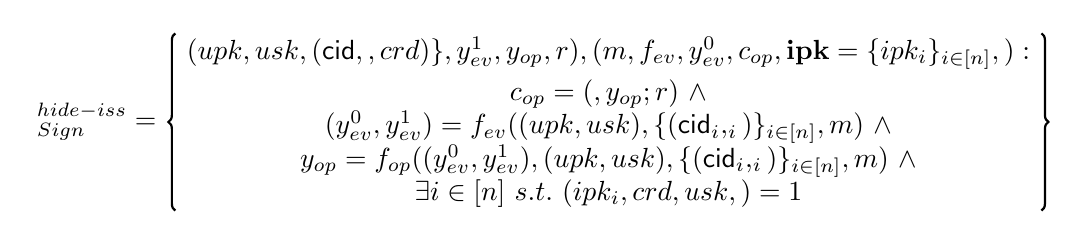
\begin{tikzpicture}

  \node (sign) at (-6.50,6.625) { $\NIZKRel^{hide-iss}_{\Sign} = $ };
  \node (sign2) at (0.00,7.50) {
    $(\upk,\usk,(\cid,\attrs,\cred)\rbrace,\yeval^1,\yinsp,r),
    (\msg,\feval,\yeval^0,\cinsp,\sipk=\lbrace\ipk_i
    \rbrace_{i\in[n]},\Eek):$
  };
  \node[align=center] (sign3) at (0.00,6.35) {
%    $\upk = \CCommit(\usk;0) \land \Ccom = \CCommit(\usk;r) \land
    $\cinsp = \EEnc (\Eek,\yinsp;r)~\land$ \\
    $(\yeval^0,\yeval^1) =
    \feval((\upk,\usk),\lbrace (\cid_i,\attrs_i) \rbrace_{i\in[n]},\msg)~\land$ \\ 
    $\yinsp = \finsp((\yeval^0,\yeval^1),(\upk,\usk),
    \lbrace (\cid_i,\attrs_i) \rbrace_{i\in[n]},\msg)~\land$ \\
    $\exists i\in[n]~\suchthat~%\ipk_i=\upk \land
    \SBCMVerify(\ipk_i,\cred,\usk,\attrs) = 1$
  };
  \draw [thick,decorate,decoration={brace}] (-5.50,5.50) -- (-5.50,7.75);
  \draw [thick,decorate,decoration={brace}] (5.50,7.75) -- (5.50,5.50);

\end{tikzpicture}

%%% Local Variables:
%%% mode: latex
%%% TeX-master: "../uas-paper"
%%% End:

  }
  \caption{$\RelSig^{hide-iss}$ relation for \CUASGenHideIss.}
  \label{fig:nizk-ring}
\end{figure}

\paragraph{\CUASGenInt: Interactive Credential Presentations with replay
  protection.}
%
In group signatures, signing and verification are non-interactive processes;
whereas in anonymous credentials, it is an interactive protocol. While
\CUASGen targets the non-interactive approach, we sketch how to transform it
into an interactive protocol with replay protection.

Modelling-wise, this requires to replace the \Sign and \Verify functions with
an interactive protocol $\langle 1/0,(\yeval,\utrans_{\Sig})/\bot \rangle \gets
\langle\Sign(\usk,\opk,\sCred,\msg,\feval), \Verify(\opk,\sipk,\msg,\feval)
\rangle$,
where $\utrans_{\Sig}$ is the transcript of the protocol, and is logged now in
an equivalent of the \SIG table (\CSIG for challenge transcripts). The \SIGN
and \CHALb oracles now also accept a random value from the adversary, but
are otherwise adapted in the natural way, where the signer is always honest, but
the verifier is played by the adversary (e.g., similar to the \OBTAIN oracle).

The construction is also simple. Basically, prior to signing the message, we
require that the verifier sends to the user a number picked uniformly at random
from an appropriate domain, which must be concatenated to the signed message. If
there is no need to actually sign a message, then the message is set to an empty
string, and the user only signs the random number.
%
If the logic within the \feval and \finsp functions needs to ignore the random
value $rnd$ sent by the verifier, note that it is trivial to transform these
functions so that they treat the message concatenated with $rnd$ as a pair
$(\msg,rnd)$, and simply ignore $rnd$.

We sketch security of \CUASGenInt in \appref{sapp:sec-interactive} assuming
the same security properties as in \UAS. Note that extra properties may be
needed in some scenarios. For instance, informally, the non-interactive version
does not provide deniability and, thus, our transform to the interactive case
does not provide it either. On the other hand, transferability is possible in
both cases, which may be useful, e.g., in situations where chaining multiple
requests is needed.
%
However, since probably the most common use of interactive presentations simply
worries about preventing replay attacks, we leave a more detailed analysis of
possible transforms (still meeting the \UAS model) out of scope.

%%% Local Variables:
%%% mode: latex
%%% TeX-master: "uas-paper"
%%% End:

\section{Relationships with Other Schemes}
\label{sec:relationships}

% [11 pages max]

In the following, to showcase the generality of \UAS and \CUASGen, we reproduce
models of related schemes in the literature.
Then, we give concrete $(\fissue,\feval,\finsp)$-\CUASGen restrictions and prove
that they securely instantiate the models for the presented schemes, if the
corresponding \CUASGen restriction is a secure \UAS construction. Concretely,
we rely on the functions described in \figref{fig:func-restrictions}. Observe
that all the \fissue functions listed in \figref{fig:func-restrictions} are
\UAS-acceptable. Specifically, $\fissue^1$ and $\fissue^{\sring}$ are trivially
\UAS-acceptable (for $\rngfissue = \bin$); whereas $\fissue^{single,H,I}$ is
\UAS-acceptable if $F$ is a secure PRF \cite{kl14}.

\begin{figure}[ht!]
  \centering
  \scalebox{0.85}{
    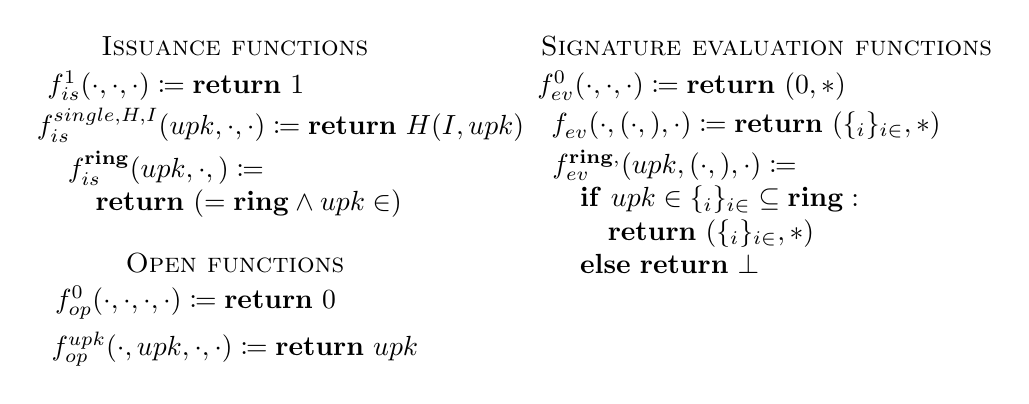
\begin{tikzpicture}

  \pgfdeclarelayer{bg}    % declare background layer
  \pgfsetlayers{bg,main}  % set the order of the layers (main is the standard layer)

  \node (issue) at (0.00,5.00) { \sc Issuance functions };
  \node (sign) at (6.75,5.00) { \sc Signature evaluation functions };  
  \node (open) at (0.00,2.25) { \sc Open functions };

  % Issue functions
  \node (fissue1) at (-0.75,4.50) {
    $\fissue^1(\cdot,\cdot,\cdot) \coloneqq \pcreturn 1$
  };
  \node (fissue2) at (0.58,4.00) {
    $\fissue^{single,H,I}(\upk,\cdot,\cdot) \coloneqq \pcreturn H(I,\upk)$
  };
  \node[align=left] (fissue3) at (0.00,3.25) {
    $\fissue^{\sring}(\upk,\cdot,\attrs) \coloneqq$ \\
    \hspace*{1em}$\pcreturn (\attrs = \sring \land \upk \in \attrs)$
  };

  % Signature evaluation functions
  \node (fsign1) at (5.80,4.50) {
    $\feval^0(\cdot,\cdot,\cdot) \coloneqq \pcreturn (0,\ast)$
  };
  \node[align=left] (fsign2) at (6.55,4.00) {
    $\feval^{\dattrs}(\cdot,(\cdot,\attrs),\cdot) \coloneqq
    \pcreturn (\lbrace \attrs_i \rbrace_{i\in \dattrs},\ast)$
  };
  \node[align=left] (fsign3) at (5.98,2.90) {
    $\feval^{\sring,\dattrs}(\upk,(\cdot,\attrs),\cdot) \coloneqq$ \\
    \hspace*{1em}$\pcif \upk \in \lbrace \attrs_i \rbrace_{i\in\dattrs}
    \subseteq \sring:$ \\
    \hspace*{2em}$\pcreturn (\lbrace \attrs_i \rbrace_{i\in\dattrs},\ast)$ \\
    \hspace*{1em}$\pcelse \pcreturn \bot$
  };
  % \node[align=left] (fsign4) at (6.65,1.20) {
  %   $\feval^{\dattrs,F,V,L}(\upk,((\cidi,\cidu),\attrs),\cdot) \coloneqq$ \\
  %   \hspace*{1em}$\pcif F(V,\cidi) \in L \lor F(V,\cidu) \in L:$ \\
  %   \hspace*{2em}$\pcreturn \bot$ \\
  %   \hspace*{1em}$\pcelse \pcreturn (\lbrace \attrs_i \rbrace_{i\in \dattrs},V)$
  % };
  %   \node[align=left] (fsign5) at (7.00,-0.65) {
  %   $\feval^{g,MPS}(\upk,\lbrace (\cid_i,\attrs_i) \rbrace_{i\in[n]},\msg) \coloneqq$ \\
  %   \hspace*{1em}$\pcif g(\upk,\lbrace (\cid_i,\attrs_i) \rbrace_{i\in[n]},
  %   \msg) = 0:$ \\
  %   \hspace*{2em}$\pcreturn \bot$ \\
  %   \hspace*{1em}$\pcelse$ \\
  %   \hspace*{2em}$\pcreturn (\ast,g(\upk,\lbrace(\cid_i,\attrs_i)
  %   \rbrace_{i\in[n]},\msg))$
  % };

  % Open functions
  \node (fopen1) at (-0.50,1.75) {
    $\finsp^0(\cdot,\cdot,\cdot,\cdot) \coloneqq \pcreturn 0$
  };
  \node (fopen2) at (0.00,1.15) {
    $\finsp^{\upk}(\cdot,\upk,\cdot,\cdot) \coloneqq \pcreturn \upk$
  };
  % \node[align=left] (fopen3) at (0.65,0.00) {
  %   $\finsp^{F}((\yeval^0,\yeval^1),\cdot,((\cidi,\cidu),\attrs),\cdot)
  %   \coloneqq$ \\
  %   \hspace*{1em}$\pcif \yeval^0 \neq 0:$\\
  %   \hspace*{2em}$\pcreturn (F(\yeval^1,\cidi),F(\yeval^1,\cidu))$ \\
  %   \hspace*{1em}$\pcelse \pcreturn 0$
  % };
  % \node[align=left] (fopen4) at (0.15,-1.30){
  %   $\finsp^{h,MPS}((\cdot,\yeval^1),\upk,\cid,\attrs,\cdot) \coloneqq$ \\
  %   \hspace*{1em}$\pcreturn h(\yeval^1,\upk,\cid,\attrs)$
  % };
  
  % \draw[draw=black,thick] (5.65,2.29) rectangle ++(1.43,0.44);
  % \draw[draw=black,dashed,thick] (1.80,1.09) rectangle ++(1.75,0.44);
  % \draw[draw=black,dotted,thick] (3.85,1.09) rectangle ++(2.30,0.44);
    
\end{tikzpicture}

%%% Local Variables:
%%% mode: latex
%%% TeX-master: t
%%% End:

  }
  \caption{Functions for the \CUASGen restrictions described next.
    For readability, we use ``$\cdot$'' to denote input arguments that are
    ignored; and ``$\ast$'' to denote output values that can be set to anything
    (but should be ignored). $\bot$ means that the function fails.}
  \label{fig:func-restrictions}
\end{figure}

\subsection{Group Signatures}
\label{ssec:related-models-gs}

We adopt the model in \cite{bsz05}. In this abstraction of group signatures, the
opener returns an index uniquely identifying the group member that created a
signature, along with a correctness proof. For ease of exposition, assume that,
w.l.o.g., this index is just the public key that the group member generates
randomly when joining the group\footnote{The user public key is assumed to be
  accessible from a public table in \cite{bsz05}, so it is easy to translate the
  public key into an index, if needed.}. A group signature scheme, according to
\cite{bsz05}, is composed of $KeyGen$, \UKeyGen, \Sign, \Verify, \Open and
\Judge algorithms, as well as an $\langle\Obtain,\Issue\rangle$ interactive
protocol. Their intuition is similar to that of \UAS, so we refer to
\cite{bsz05} for detailed descriptions. For ease of reference, we replicate the
security games in \figref{fig:model-gs}.

\begin{figure}[ht!]
  \centering
  \scalebox{0.85}{      
    \begin{minipage}[t]{0.45\textwidth}        
      \procedure[linenumbering]{$\Exp^{anon-b}_{\adv,gs}(1^\secpar)$}{%
        (\gpk,\isk,\osk) \gets KeyGen(1^\secpar) \\
        d \gets \adv^{\mathcal{O}_{anon}}(\gpk,\isk) \\
        \pcreturn d 
      }
      
      \vspace*{3em}
      
      \procedure[linenumbering]{$\Exp^{frame}_{\adv,gs}(1^\secpar)$}{%
        (\gpk,\isk,\osk) \gets KeyGen(1^\secpar) \\
        (\msg,\sig,\upk,\tau) \gets \adv^{\mathcal{O}_{frame}}
        (\gpk,\osk,\isk) \\
        \pcif \Verify(\gpk,\msg,\sig) = 0: \pcreturn 0 \\
        \pcreturn \upk \in \HU \land \PRVUK[\upk] \neq \bot \land
        \Judge(\gpk,\upk,\msg,\sig,\tau) = 1~\land \\
        \pcind \adv~\textrm{did not query}~USK(\upk)~\textrm{or}~
        GSig(\PRVUK[\upk],\msg)
      }       
    \end{minipage}
  }
  \scalebox{0.85}{      
    \begin{minipage}[t]{.55\textwidth}
      \procedure[linenumbering]{$\Exp^{trace}_{\adv,gs}(1^\secpar)$}{%
        (\gpk,\isk,\osk) \gets KeyGen(1^\secpar) \\
        (\msg,\sig) \gets \adv^{\mathcal{O}_{trace}}(\gpk,\osk) \\
        \pcif \Verify(\gpk,\msg,\sig) = 0: \pcreturn 0 \\
        (\upk, \tau) \gets \Open(\gpk,\osk,\trans,\msg,\sig) \\
        \pcreturn \upk \notin \HU \cup \CU \lor \Judge(\gpk,\upk,\msg,\sig,\tau)
        = 0
      }       
    \end{minipage}      
  }
  \caption{Security games for group signatures \cite{bsz05}, only with minor    
    ``harmless'' edits to compare easier with \CUASGS. Concretely, since we
    output {\upk}s instead of indexes, $i=0$ in the traceability game now reads
    $\upk \notin \HU \cup \CU$. For the oracles' definitions, check the
    referenced paper.
    $\mathcal{O}_{anon} \gets \lbrace \oracle{Ch},\oracle{Open},\oracle{SndToU},
    \oracle{WReg},\oracle{USK},\oracle{CrptU} \rbrace$,
    $\mathcal{O}_{trace} \gets \lbrace \oracle{SndToI},\oracle{AddU},
    \oracle{RReg},\oracle{GSig},\oracle{USK},\oracle{CrptU} \rbrace$,
    and $\mathcal{O}_{frame} \gets \lbrace \oracle{SndToU},\oracle{WReg},
    \oracle{GSig},\oracle{USK},\oracle{CrptU} \rbrace$.
  }
  \label{fig:model-gs}  
\end{figure}

\subsubsection{\CUASGS construction.} %
We show that the $(\fissue^{single,H,I},\feval^0,\finsp^{\upk})$-\CUASGen
restriction, is a secure group signature scheme according to \cite{bsz05}.
As stated, $\fissue^{single,H,I}$ is an \UAS-acceptable function if $F$ is a
PRF. In that case, its output is a random-looking string that depends on the
user public key \upk, and a string $I$ uniquely identifying the issuer. Thus, it
will be the same per $(\upk,I)$ pair, and can be used by issuer $I$ to prevent
issuing more than one credential per user. Basically, the issuer maintains a
list of received $\yissue = F(\upk,I)$ values, and rejects issuing a credential
for already existing ones. From this, the GS algorithms are as
follows:

\begin{description}
\item[$(\gpk,\isk,\osk) \gets KeyGen(1^\secpar)$.] Runs \Setup from \CUASGen,
  and one instance of \KeyGen and \ISet with $\fissue^{single,H,I}$ (both for
  the same user, who will be the only issuer in the GS scheme) and \OKeyGen.
  Assigns the public keys to \gpk.
\item[$(\upk,\usk) \gets \UKeyGen(1^\secpar)$.] Runs \KeyGen from \CUASGen.
\item[$\langle \cred,\utrans \rangle \gets
  \langle\Obtain(\usk,\ipk),\Issue(\isk,\upk)\rangle$.] Runs $\langle\Obtain,
  \Issue\rangle$ as in \CUASGen, with $\attrs \gets \emptyset$. Upon receiving
  the \yissue value, the issuer checks if it already exists in a list $L$
  (initially set to $\emptyset$); if it exists, aborts issuance. Otherwise, it
  completes the protocol and adds $\yissue$ to $L$. It is responsibility of the
  issuer to maintain $L$.
\item[$\sig \gets \Sign(\gpk,\cred,\msg)$.] Parses \gpk as $(\ipk,\opk)$, and
  runs $(\sig,0) \gets \Sign(\usk,\opk,\cred,\msg,\feval^0)$ from \CUASGen,
  where $\yeval = 0$ is the constant output of $\feval^0$.
\item[$1/0 \gets \Verify(\gpk,\sig,\msg)$.] Parses \gpk as $(\ipk,\opk)$, and
  returns whatever $\Verify(\opk,\ipk,\sig,0,\msg,\feval^0)$ from \CUASGen
  outputs.
\item[$(\upk,\pi) \gets \Open(\gpk,\osk,\trans,\sig,\msg)$.] Parses \gpk as
  $(\ipk,\opk)$, and returns whatever \CUASGen outputs in $\Open(\osk,\ipk,\sig,
  0,\msg,\feval^0)$. Internally, the call to \Open runs $\finsp^{\upk}$.
\item[$1/0 \gets \Judge(\gpk,\pi,\upk,\sig,\msg)$.] Parses \gpk as $(\ipk,
  \opk)$, and returns whatever \CUASGen outputs in $\Judge(\opk,\upk,\pi,\sig,
  0,\msg)$.
\end{description}

\paragraph{Security of \CUASGS.} %
Our \CUASGS construction is an anonymous, traceable, and non-frameable group
signature scheme, according to the model in \cite{bsz05}. For space constraints,
proofs are deferred to \appref{app:related-proofs}.

% \begin{theorem}[Anonymity of \CUASGS]
%   If the base \CUASGen construction has signature anonymity according to
%   \defref{def:sign-anonymity-uas}, then \CUASGS is an anonymous group signature
%   scheme.
% \end{theorem}

% \begin{theorem}[Traceability of \CUASGS]
%   If the base \CUASGen construction is unforgeable according to
%   \defref{def:forge-uas}, then \CUASGS is a traceable group signature scheme.
% \end{theorem}

% \begin{theorem}[Non-frameability of \CUASGS]
%   If the base \CUASGen construction is non-frameable according to
%   \defref{def:frame-uas}, then \CUASGS is a non-frameable group signature
%   scheme.
% \end{theorem}

\subsection{Ring Signatures}
\label{ssec:related-models-rs}

We adopt the model in \cite{bkm06}, where security of ring signatures is
defined according to the games in \figref{fig:model-rs}. A ring signature
scheme consists of three algorithms $(KeyGen,Sign,Verify)$. Roughly,
$((\pk_1,\sk_1),\dots,(\pk_n,\sk_n)) \gets KeyGen(1^\secpar)$ produces $n$
signing key pairs, $\sig \gets Sign(\sk_i,R,\msg)$ creates a signature for
anonymity set $R \subseteq \lbrace \pk_1, \dots, \pk_t \rbrace$, using secret
key $\sk_i$, associated to some $\pk_i \in R$; and $1/0 \gets Verify(R,\sig,
\msg)$ checks if \sig is a valid signature over \msg for ring $R$. We refer
to \cite{bkm06} for details on the syntax and definitions.

\begin{figure}[ht!]
  \centering
  \scalebox{0.85}{      
    \begin{minipage}[t]{0.55\textwidth}        
      \procedure[linenumbering]{$\Exp^{anon-b}_{\adv,rs}(1^\secpar)$}{%
        ((\pk_1,\sk_1),\dots,(\pk_n,\sk_n)) \gets KeyGen(1^\secpar) \\
        (i_0,i_1,R,\msg,\st) \gets \adv^{\oracle{SIGN}}(\pk_1,\dots,\pk_n) \\
        \pcif R \not\subseteq \lbrace \pk_i \rbrace_{i\in[n]} \lor
        \lbrace \pk_{i_0},\pk_{i_1} \rbrace \not\subseteq R~\lor \\ %\\
        \pcind i_0 = i_1: \pcreturn \bot \\
        \sig \gets Sign(\sk_{i_b},R,\msg) \\
        b^* \gets \adv(\sig,\st) \\
        \pcreturn b^*
      }        
    \end{minipage}
  }
  \scalebox{0.85}{      
    \begin{minipage}[t]{.5\textwidth}
      \procedure[linenumbering]{$\Exp^{forge}_{\adv,rs}(1^\secpar)$}{%
        ((\pk_1,\sk_1),\dots,(\pk_n,\sk_n)) \gets KeyGen(1^\secpar) \\
        (R,\sig,\msg) \gets \adv^{\oracle{SIGN},\oracle{CORR}}
        (\pk_1,\dots,\pk_n) \\
        \pcif Verify(R,\sig,\msg) = 0: \pcreturn 0 \\
        \pcreturn (R \subseteq \lbrace \pk_i \rbrace_{i\in[n]} \setminus
        CU~\land \\
        \pcind \adv~\textrm{never queried}~SIGN(\cdot,R,\msg))
      }       
    \end{minipage}      
  }
  \caption{Security games for ring signatures \cite{bkm06}. The $\oracle{SIGN}$
    oracle accepts $(i,R,\msg)$ tuples, with $pk_i \in R$, adds the tuple to a
    list of queries, and returns $\sig \gets Sign(\sk_i,R,\msg)$.
    $\oracle{CORR}$ accepts an index $i$, and leaks $\sk_i$. Corrupted users are
    added to $CU$.}
  \label{fig:model-rs}  
\end{figure}


\subsubsection{\CUASRing Construction.} %
We can use a $(\fissue^{\sring},\feval^{\sring,\dattrs},\finsp^0)$-restriction
of \CUASGenHideIss to build a ring signature scheme according to the model
in \figref{fig:model-rs}. In a nutshell, we let users self-issue
credentials where the attributes are (a subset of encodings of) the public keys
of the users in the system -- including their own public key. Then, a ring
signature is just a \CUASGenHideIss signature that reveals a subset of
the attributes -- i.e., a subset of the keys of the users in the system. In more
detail, the construction is as follows:

% \begin{align}
%   & \NIZKRel_{\Sign}^{prv} \coloneqq \lbrace (\usk,\cred,\yeval^1,\yinsp,r,r',
%     \ipk),(\msg,\feval,\yeval^0,\ceval,\cinsp,\Eek,\widetilde{\Eek},\sring): \nonumber \\
%   & \hspace*{6.405em}\ceval = \EEnc(\widetilde{\Eek},\yeval^1;r) \land
%     \cinsp = \EEnc(\Eek,\yinsp;r') \land \nonumber \\
%   & \hspace*{6.40em}(\yeval^0,\yeval^1) = \feval(\usk,\cred,\msg) \land
%     \yinsp = \finsp((\yeval^0,\yeval^1),\usk,\cred,\msg) \nonumber \\
%   & \hspace*{6.40em}\exists \ipk \in \sring~\suchthat~\SBCMVerify(\ipk,\cred,\usk,
%     \sring) = 1) \rbrace \label{eq:sign-prv}
% \end{align}

% From it, we show that the $(\fissue^{\sring},\feval^{\attrs},\finsp^0)$-
% $\CUASGen^{\Sign-prv}$ restriction, is a secure ring signature scheme. We
% restrict to one credential per signature.

\begin{description}
%\item[$\parm \gets \Setup(\secpar,\AttrSpace)$.] As in \CUASGenHideIss.
\item[$((\pk_1,\sk_1),...,(\pk_n,\sk_n)) \gets KeyGen(\secpar)$.] Runs
  $\parm \gets \Setup(\secpar)$ from \CUASGenHideIss. For each of
  the $i \in [n]$ users to generate, run $(\upk_i,\usk_i) \gets \KeyGen(\parm)$,
  and $\ipk_i \gets \ISet((\upk_i,\usk_i),\fissue^{\sring})$, where $\sring =
  \lbrace \upk_i \rbrace_{i\in[n]}$. Run also $(\opk,\osk) \gets \OKeyGen(\parm,
  \finsp^0)$. Set $\pk_i \gets (\ipk_i,\opk)$ and $\sk_i \gets \usk_i$, for
  $i\in[n]$.
\item[$\Sig \gets \Sign(\sk_i,R,\msg).$]
  The signing user, with $\sk_i=\usk$ and $\pk_i=(\ipk_i,\opk)$ for some $i \in
  [n]$ where $\pk_i \in R$, first acts both as user and issuer to self-issue a
  credential \Cred over an attribute set \attrs such that $\attrs \subseteq
  \sring$. The user picks some \dattrs such that $\dattrs \subseteq [|\attrs|]$,
  and computes the ring signature by running $\Sig = (\sig,\yeval) \gets
  \Sign(\usk,\opk,\Cred,\msg,\feval^{\sring,\dattrs})$ from
  \CUASGenHideIss. Note that \dattrs defines the public keys within
  $\attrs \subseteq \sring$ to be revealed through \yeval.
\item[$1/0 \gets Verify(R,\Sig,\msg)$.] Parses \Sig as $(\sig,\yeval)$ and
  runs $\Verify(\opk,\yeval,\Sig,\msg,\feval^{\sring,\dattrs})$ as in
  \CUASGenHideIss. Note that, in valid signatures, $\yeval = \lbrace
  \ipk_i\rbrace_{i\in\dattrs}$.
\end{description}

%Note that by using, e.g., $\finsp^{\upk}$, we essentially get a ring signature
%scheme with linkability via an opener.

\paragraph{Security of \CUASRing.} %
Our \CUASRing construction is an anonymous and unforgeable ring signature
scheme, according to the model in \cite{bkm06}. For space constraints,
proofs are deferred to \appref{app:related-proofs}.

% \begin{theorem}[Anonymity of \CUASRing]
%   If the base \CUASGenHideIss construction has signature anonymity
%   according to \defref{def:sign-anonymity-uas}, then \CUASRing is an anonymous
%   ring signature scheme.
% \end{theorem}

% \begin{theorem}[Unforgeability of \CUASRing]
%   If the base \CUASGenHideIss construction is non-frameable according to
%   \defref{def:frame-uas}, then \CUASRing is an unforgeable ring signature
%   scheme.
% \end{theorem}

\subsection{Anonymous Credentials}
\label{ssec:related-models-ac}

We adopt the model in \cite{fhs19}, for anonymous credentials with selective
disclosure, which restricts to one credential per presentation. Therein, an
anonymous credential scheme is defined via $OrgKeyGen$ (which we rename to
$IssKeyGen$), and $UserKeyGen$ algorithms, and $\langle Obtain,Issue\rangle$
and $\langle Show,Verify \rangle$ interactive protocols. We
refer to \cite{fhs19} for the full details. For ease of reference, we summarize
the security definitions in \figref{fig:model-ac}.% , with inocuous
% adaptations to make them more suitable for comparison with our definitions --
% namely, we explicitly add a common setup process which is part of $IssKeyGen$
% in \cite{fhs19}.

\begin{figure}[ht!]
  \centering
  \scalebox{0.85}{      
    \begin{minipage}[t]{0.5\textwidth}        
      \procedure[linenumbering]{$\Exp^{anon-b}_{\adv,ac}(1^\secpar)$}{%
 %       \parm \gets \Setup(1^\secpar) \\
        (\ipk,\isk) \gets IssKeyGen(1^\secpar) \\        
        b^* \gets \adv^{\oracle{HU},\oracle{CU},\oracle{Obtain},
          \oracle{Show},\oracle{LoR}}(\isk) \\
        \pcreturn b^*
      }        
    \end{minipage}
  }
  \scalebox{0.85}{      
    \begin{minipage}[t]{.5\textwidth}
      \procedure[linenumbering]{$\Exp^{forge}_{\adv,ac}(1^\secpar)$}{%
%        \parm \gets \Setup(1^\secpar) \\
        (\ipk,\isk) \gets IssKeyGen(1^\secpar) \\        
        (D,\st) \gets \adv^{\oracle{HU},\oracle{CU},\oracle{ObtIss},
          \oracle{Issue},\oracle{Show}}(\ipk) \\
        \langle \cdot,(b,\utrans) \rangle
        \gets \langle \adv(\st),\Verify(\ipk,D) \rangle \\
        \pcreturn (b = 1 \land \nexists j~\suchthat \\
        \pcind (\OWNR[j] \in \CU
        \land D \subseteq \ATTR[j])) % \forall j, \OWNR[j] \in \CU
        % \implies D \not\subseteq \ATTR[j]: \\
        %\pcind \pcreturn 1 \\
        %\pcreturn 0
      }       
    \end{minipage}      
  }
  \caption{Games for anonymous credentials with selective disclosure
    \cite{fhs19}. \OWNR, \ATTR, and the oracles, are essentially as in
    \UAS. \adv~wins $\Exp^{forge}_{\adv,ac}$ if it authenticates successfully
    while revealing attributes not contained in adversarially controlled
    credentials.}
  \label{fig:model-ac}  
\end{figure}

\subsubsection{\CUASAC Construction.} %
We show that a $(\fissue^1,\feval^{\dattrs},\finsp^0)$-\CUASGenInt
restriction, is a secure anonymous credential scheme according to the model in
\cite{fhs19}. We first quickly define the algorithms, and then prove security.

\begin{description}
% \item[$\parm \gets \Setup(1^\secpar)$.] Runs $\parm' \gets \Setup(1^\secpar,
%   \AttrSpace)$ and $(\opk,\osk) \gets \OKeyGen(\parm',\finsp^0)$ from our
%   \CUASGen construction. Returns $\parm \gets (\parm',\opk)$.
\item[$(\ipk,\isk) \gets IssKeyGen(\parm)$.] From \CUASGenInt, run $\parm'
  \gets \Setup(1^\secpar)$ and $(\opk,\osk) \gets \OKeyGen(\parm',
  \finsp^0)$, and set $\parm \gets (\parm',\opk)$. Run $(\upk,\usk) \gets
  \KeyGen(\parm')$ and $\ipk \gets \ISet(\upk,\usk,\fissue^1)$. Set $\isk \gets
  \usk$.
\item[$(\upk,\usk) \gets UserKeyGen(\ipk)$.] Runs \KeyGen from \CUASGenInt.
\item[$\langle \cred/\bot,\top/\bot \rangle \gets
  \langle \Obtain(\usk,\ipk,\attrs),\Issue(\isk,\upk,\attrs) \rangle$.]
  Runs $\langle \Obtain,\Issue \rangle$ from \CUASGenInt.
\item[$\langle 1/0,((\yeval,\utrans)/(0,\utrans)\rangle
  \gets \langle Show(\ipk,\attrs,\dattrs,
  \cred),\Verify(\ipk,\dattrs) \rangle$.]
  Runs the interactive $\langle \Sign, \Verify\rangle$ of  \CUASGenInt,
  using $\feval^{\dattrs}$ as signature evaluation function, and $\finsp^0$ as
  open function, with \opk from \parm as opener public key. The \yeval value
  output by the verifier, when it accepts, is the $\yeval^0$ value produced by
  \Sign in \CUASGenInt.
\end{description}

\paragraph{Security of \CUASAC.} %
Our \CUASAC construction is an anonymous and unforgeable anonymous credential
scheme, according to the model in \cite{fhs19}. For space constraints,
proofs are deferred to \appref{app:related-proofs}.

% \begin{theorem}[Anonymity of \CUASAC]
%   \label{thm:anon-cuasac}
%   If the base \CUASGenInt construction has signature anonymity according to
%   \defref{def:sign-anonymity-uas}, then \CUASAC is an anonymous AC scheme
%   according to \cite{fhs19}.
% \end{theorem}

% \begin{theorem}[Unforgeability of \CUASAC]
%   \label{thm:forge-cuasac}
%   If the base \CUASGenInt construction is unforgeabile according to
%   \defref{def:forge-uas}, then \CUASAC is an unforgeable AC scheme.
% \end{theorem}

%%% Local Variables:
%%% mode: latex
%%% TeX-master: "uas-paper"
%%% End:

\section{Conclusion}
\label{sec:conclusion}

We present a general model for privacy-preserving signatures and authentication,
and provide a generic construction, secure in our model, that allows
different privacy-vs-utility tradeoffs to be reached.
%
Then, we prove that well-known schemes are special cases of our generic
construction. The implied schemes include group signatures, anonymous
credentials (with and without revocation), ring signatures, or the recently
proposed multimodal private signatures.

The flexibility of our model is achieved via functional placeholders that
modulate the behaviour at credential issuance time, the utility
information ``leaked'' along with the produced signatures, and the utility
information extractable from already produced signatures. These functions are
computed by the users themselves, who need to prove correct computation.
Our setting also combines features of anonymous credential schemes, like
attribute-based credentials and multiple issuers, which we extend with openers
(like in group signatures), but also enabling that multiple openers coexist.
This further increases the flexibility, by removing the tight issuer-opener
coupling in previous works.

For future work, an obvious line is to come up with (and implement) concrete
instantiations of our generic construction in order to evaluate efficiency in
real-world use cases. Also, it may be interesting to come up with alternative
generic constructions -- for instance, based on structure-preserving signatures.
%
Finally, in this work we focus only on utility over \emph{one} signature. But
extending our model and constructions to span utility over \emph{multiple}
signatures promises to be interesting, both regarding its modelling and the
potential use cases.


%%% Local Variables:
%%% mode: latex
%%% TeX-master: "uas-paper"
%%% End:


\bibliographystyle{splncs04}
\bibliography{uas-paper}

\appendix

\section{Cryptographic Building Blocks}
\label{app:crypto-building-blocks}

\subsection{Digital Signatures}
\label{sapp:digital-signatures}

We rely on digital signatures as a core building block. A digital signature
provides the functionality defined by the following syntax:

\begin{description}
\item[$\Sparm \gets \SSetup(\Ssecpar)$.] It produces public parameters for the
  other algorithms, given an input security parameter \Ssecpar.
\item[$(\Svk,\Ssk) \gets \SKeyGen(\Sparm)$.] Generates a verification-signing
  key pair.
\item[$\Ssig \gets \SSign(\Ssk,\msg)$.] Signs message \msg with signing key
  \Ssk, producing signature \Ssig,  
\item[$1/0 \gets \SVerify(\Svk,\Ssig,\msg)$.] Checks whether \Ssig is a valid
  signature over \msg, under verification key \Svk.
\end{description}

A digital signature scheme is correct if honestly generated signatures, using
honestly generated key pairs, are always accepted by \SVerify. 
%
A digital signature scheme \S has existential unforgeability if, for all p.p.t.
adversaries $\adv$, $\Pr[\ExpEUF(\Ssecpar) = 1]$ is a negligible function of the
security parameter.

\begin{figure}[ht!]
  \begin{minipage}[t]{\textwidth}
    \centering
    \procedure{$\ExpEUF(\Ssecpar)$}{%
      \Sparm \gets \SSetup(\Ssecpar) \\
      (\Svk,\Ssk) \gets \SKeyGen(\Sparm) \\
      (\Ssig,\msg) \gets \adv^{\SSign(\Ssk,\cdot)}(\Svk) \\
      \pcif \SVerify(\Svk,\Ssig,\msg) = 0: \pcreturn 0 \\
      \pcif \msg~\textrm{was not queried to \SSign}: \pcreturn 1 \\
      \pcreturn 0
    }
  \end{minipage}
  \label{fig:euf-game}
  \caption{Existential Unforgeability Game.}
\end{figure}

\subsection{Public-Key Encryption}
\label{sapp:pk-encryption}

A public-key encryption scheme is defined by the following algorithms:

\begin{description}
\item[$\Eparm \gets \ESetup(\Esecpar)$.] Produces public parameters \Eparm given
  a security parameter \Esecpar.
\item[$(\Eek,\Edk) \gets \EKeyGen(\Eparm)$.] Given public parameters \Eparm,
  produces an encryption-decryption keypair $(\Eek,\Edk)$.
\item[$\Ec \gets \EEnc(\Eek,\msg)$.] Encrypts message \msg with encryption key
  \Eek, producing ciphertext \Ec.
\item[$\msg \gets \EDec(\Edk,\Ec)$.] Decrypts ciphertext \Ec with decryption key
  \Edk.
\end{description}

A public-key encryption scheme is correct if, given a honestly generated key
pair $(\Eek,\Edk)$, produced with honestly generated parameters \Eparm,
$\Pr[\EDec(\Edk,\EEnc(\Eek,\msg))=\msg] = 1$ with overwhelming probability.

A public-key encryption scheme has IND-CCA2 security if
$\Pr[\ExpINDCCAiio(\Esecpar) = 1] - \Pr[\ExpINDCCAiiz(\Esecpar) = 1]|$ is
a negligible function of \Esecpar, for any p.p.t. adversary \adv, where
\ExpINDCCAiib is as defined in \figref{fig:indcca2-game}.

\begin{figure}[ht!]
  \begin{minipage}[t]{\textwidth}
    \centering      
    \procedure{$\ExpINDCCAiib(\Esecpar)$}{%
      \Eparm \gets \ESetup(\Esecpar) \\
      (\Eek,\Edk) \gets \EKeyGen(\Eparm) \\
      b^* \gets \adv^{\ELR(b,\cdot,\cdot),\EDEC(\Edk,\cdot)}(\Eek),
      ~\textrm{where:} \\
      \pcind \ELR(b,\msg_0,\msg_1)~\textrm{returns}~\EEnc(\Eek,\msg_b),
      ~\textrm{and} \\
      \pcind \EDEC(\Edk,\Ec)~\textrm{returns}~\EDec(\Edk,\Ec) \\
      \pcif \EDEC~\textrm{has been called with an output of \ELR, abort} \\
      \pcreturn b^*
    }
  \end{minipage}
  \label{fig:indcca2-game}
  \caption{IND-CCA2 Game.}
\end{figure}

\subsection{Commitments}
\label{sapp:commitments}

A commitment scheme is defined by the following algorithms:

\begin{description}
\item[$\Cparm \gets \CSetup(\Csecpar)$.] Given a security parameter \Csecpar,
  returns the public parameters \Cparm to commit messages.
\item[$\Ccom \gets \CCommit(\Cparm,\msg;r)$.] Given the public parameters and
  a message \msg, outputs a commitment \Ccom to \msg, for which randomness $r$
  from some predefined randomness space $\mathcal{R}$ is used.
\end{description}

Opening a commitment \Ccom means revealing the message \msg and randomness $r$
that were used to produce \Ccom. Commitment schemes are required to be binding
and (usually) hiding:

\begin{description}
\item[Binding.] Intuitively, the binding property of commitment schemes means
  that no adversary can change the message that has been committed to. More
  formally, $\Pr[\ExpComBind(\Csecpar) = 1]$ must be a negligible function of
  the security parameter.
\item[Hiding.] The hiding property captures that no adversary should be able to
  learn the message that was committed, when given only the commitment. This is
  formally defined through \ExpComHideb, where $|\Pr[\ExpComHideb(\Csecpar)=1|
  b=1] - \Pr[\ExpComHideb(\Csecpar)=1|b=0]|$ must be a negligible function of
  the security parameter.
\end{description}

\begin{figure}[ht!]
  \begin{minipage}[t]{0.5\textwidth}
    \procedure{$\ExpComBind(\Csecpar)$}{%
      \Cparm \gets \CSetup(\Csecpar) \\
      (\msg_0,r_0,\msg_1,r_1) \gets \adv(\Cparm) \\
      \Ccom_0 \gets \CCommit(\Cparm,\msg_0,r_0) \\
      \Ccom_1 \gets \CCommit(\Cparm,\msg_1,r_1) \\
      \pcif \msg_0 \neq \msg_1 \land \Ccom_0 = \Ccom_1: \pcreturn 1 \\
      \pcreturn 0
    }
  \end{minipage}
  \begin{minipage}[t]{0.5\textwidth}
    \procedure{$\ExpComHideb(\secpar)$}{%
      \Cparm \gets \CSetup(\secpar) \\
      (\msg_0,\msg_1,st) \gets \adv(\Cparm) \\
      r \getr \mathcal{R} \\
      \Ccom \gets \CCommit(\Cparm,\msg_b,r) \\
      b' \gets \adv(st,\Ccom) \\
      \pcreturn b'
    }
  \end{minipage}
  \label{fig:com-games}
  \caption{Games for commitment schemes.}
\end{figure}

\paragraph{Commitments on Blocks of Messages.} We also use an extension
of commitment schemes that allows committing to multiple messages at once. The
properties we need are the same, and their definitions are extended in the
natural way. Namely, $\CCommit$ receives a vector/block of messages, \msgset
instead of a single message. In the games, the adversary returns sets of
messages and, in the binding game, the comparison $\msg_0 \neq \msg_1$ now
compares sets $\msgset_0$ and $\msgset_1$, which must differ in at least one
element. This extension is straight-forward, for instance, from Pedersen
commitments \cite{bcc+15}.

\subsection{Simulation-Extractable Non-Interactive Zero-Knowledge
  Proofs of Knowledge}
\label{sapp:nizk}

Let \NIZKRel be an NP relation defined by pairs of elements $(\NIZKx,\NIZKw)$,
where \NIZKx is a statement and \NIZKw a witness proving that $(\NIZKx,\NIZKw)
\in \NIZKRel$. For concrete relations, we write $\NIZKRel = \lbrace (\NIZKx),
(\NIZKw): f(x,w) \rbrace$, where $f(x,w)$ is a boolean predicate denoting the
concrete conditions that \NIZKx and \NIZKw need to meet. The set of all \NIZKx
such that there exists a \NIZKw for which $(\NIZKx,\NIZKw) \in \NIZKRel$ is the
language, or \NIZKLang, for \NIZKRel. $\NIZKx \notin \NIZKLang$ means that
there is no $\NIZKw$ such that $(\NIZKx,\NIZKw) \in \NIZKRel$.

We use non-interactive zero-knowledge proofs of knowledge (NIZKPoK, or, for
short, NIZK) over NP relations, in the Common Reference String (CRS) model. A
NIZK system is a tuple $(\NIZKSetup,\NIZKProve,\NIZKVerify)$, defined as follows
\cite{gos06}:

\begin{description}
\item[$\NIZKcrs \gets \NIZKSetup(\NIZKsecpar)$.] Generates a CRS \NIZKcrs from
  security parameters \NIZKsecpar.
\item[$\NIZKproof \gets \NIZKProve(\NIZKcrs,\NIZKx,\NIZKw)$.] Given \NIZKcrs,
  statement \NIZKx, and witness \NIZKw, creates a proof \NIZKproof.
\item[$1/0 \gets \NIZKVerify(\NIZKcrs,\NIZKproof,\NIZKx)$.] Checks whether
  \NIZKproof is a valid proof for \NIZKx.
\end{description}

Any zero-knowledge proof of knowledge must meet completeness, soundness and
zero-knowledge,properties. We further need an extra property, called
\emph{simulation-extractability} \cite{cl06}, which amplifies the security
requirements of simulation soundness.
%
To define more formally the properties we need, we have to define three extra
algorithms:

\begin{description}
\item[$(\NIZKcrs,\NIZKtrap) \gets \NIZKSimSetup(\NIZKsecpar)$.] Produces a
  \NIZKcrs as the \NIZKSetup algorithm, along with a trapdoor \NIZKtrap.
\item[$\NIZKproof \gets \NIZKSim(\NIZKcrs,\NIZKtrap,\NIZKx)$.] Given a trapdoor
  \NIZKtrap produced by \NIZKSimSetup, and a statement $\NIZKx \in \NIZKLang$,
  produces a simulated proof \NIZKproof of $\NIZKx \in \NIZKLang$.
\item[$\NIZKw \gets \NIZKExtract(\NIZKcrs,\NIZKtrap,\NIZKx,\NIZKproof)$.] Given
  a trapdoor \NIZKtrap produced by \NIZKSimSetup, and a proof \NIZKproof for
  $\NIZKx \in \NIZKLang$, returns a valid \NIZKw for \NIZKx.
\end{description}

When we want to make explicit the NP relation \NIZKRel to which the previous
algorithms refer to, we use $\NIZKSetup^\NIZKRel,\NIZKProve^\NIZKRel$, 
$\NIZKVerify^\NIZKRel$, etc., and omit the \NIZK prefix and subindex when clear
from context. Altogether, the tuple $(\Setup,\Prove,\Verify,\SimSetup,\Sim,
\Extract)$ needs to meet the following properties:

\paragraph{Completeness.} %
Ensures that, for any $(\NIZKx,\NIZKw) \in \NIZKRel$, any honest prover will be
able to create a proof \NIZKproof that is accepted by any honest verifier, with
overwhelming probability. More precisely, $\Pr\lbrack\ExpNIZKComp(\NIZKsecpar)
\rbrack = 1$ with overwhelming probability, for any p.p.t. \adv, for
\ExpNIZKComp in \figref{fig:nizk-games}.

\paragraph{Soundness.} %
Ensures that no adversary can create proofs accepted by \Verify, for
statements $\NIZKx \notin \NIZKLang$, except with negligible probability. That
is, for \ExpNIZKSound as in \figref{fig:nizk-games}, $\Pr\lbrack\ExpNIZKSound
(\NIZKsecpar)\rbrack=1$ with overwhelming probability. If this holds only
against p.p.t. adversaries, we talk of Non-Interactive \emph{arguments}, while
if soundness holds even against unbounded adversaries, we talks about
Non-Interactive proofs.

\paragraph{Zero-knowledge.} %
Intuitively, captures that no information can be learned from a statement and
proof pair, beyond their validity (or not). This is captured by requiring the
adversary to distinguish between a run in the real world ($b=0$), where the
setup is done with \Setup, and $\adv$ has access to an honest prover
\Prove; and a run in an ideal world ($b=1$), where the setup is replaced by
\SimSetup, and proofs are simulated with the help of the trapdoor produced by
\SimSetup, except when $\adv$ specifies $(\NIZKx,\NIZKw) \notin \NIZKRel$. Note
that, in the context of simulation-extractable NIZK, this property not only
requires that the simulated proofs are indistinguishable to the real ones; it
also requires that \SimSetup is indistinguishable from \Setup. All this is
formalised by requiring that $|\Pr[\ExpNIZKZKb(\NIZKsecpar) = 1 | b = 1] -
\Pr[\ExpNIZKZKb(\NIZKsecpar) = 1 | b = 0]$ be a negligible function of \secpar,
where \ExpNIZKZKb is as defined in \figref{fig:nizk-games}.

\paragraph{Simulation-Extractability.} As stated, simulation-extractability
is an extension to simulation soundness. In a nutshell,
simulation-extractability requires that, even after having received a polynomial
number of simulated proofs of knowledge, no adversary can output a valid proof
of knowledge from which no witness can be extracted. It implies simulation
soundness, which ``just'' requires that no adversary can produce a valid proof
after having seen polynomially many simulated proofs (but does not guarantee
extraction). Formally, for simulation-extractability we require that
$\Pr[\ExpNIZKSimExt(\NIZKsecpar)] = 1$ is a negligible function of \secpar,
where \ExpNIZKSimExt is defined in \figref{fig:nizk-games}.

\begin{figure}[ht!]
  \begin{minipage}[t]{0.5\textwidth}
    \procedure{$\ExpNIZKComp(\NIZKsecpar)$}{%
      \NIZKcrs \gets \Setup(\NIZKsecpar) \\
      (\NIZKx,\NIZKw) \gets \adv(\NIZKcrs) \\
      \pcif (\NIZKx,\NIZKw) \notin \NIZKRel: \pcreturn 0 \\
      \NIZKproof \gets \Prove(\NIZKcrs,\NIZKx,\NIZKw) \\
      b \gets \Verify(\NIZKcrs,\NIZKproof,\NIZKx) \\
      \pcreturn b \\
    }
    \procedure{$\ExpNIZKSimExt(\NIZKsecpar)$}{%
      (\NIZKcrs,\NIZKtrap) \gets \SimSetup(\NIZKsecpar) \\
      (\NIZKx,\NIZKproof) \gets \adv^{\Sim'(\NIZKcrs,\NIZKtrap,\cdot,\cdot)}
      (\NIZKcrs) \\
      \pcind \textrm{Where}~\Sim'(\NIZKcrs,\NIZKtrap,\NIZKx,\NIZKw)~\textrm{returns} \\
      \pcind \pcind
      \Sim(\NIZKcrs,\NIZKtrap,\NIZKx)~\pcif (\NIZKx,\NIZKw) \in \NIZKRel \\
      \pcind \pcind \bot~\pcif (\NIZKx,\NIZKw) \notin \NIZKRel \\
      \NIZKw' \gets \Extract(\NIZKcrs,\NIZKtrap,\NIZKx,\NIZKproof) \\
      \pcif \Verify(\NIZKcrs,\NIZKproof,\NIZKx) = 1 \land
      (\NIZKx,\NIZKw') \notin \NIZKRel~\land \\
      \pcind \NIZKx~\textrm{was not queried to $\Sim$ via $\Sim'$}: \\
      \pcind \pcreturn 1 \\
      \pcreturn 0
    }    
  \end{minipage}
  \begin{minipage}[t]{0.5\textwidth}
    \procedure{$\ExpNIZKSound(\NIZKsecpar)$}{%
      \NIZKcrs \gets \Setup(\NIZKsecpar) \\
      (\NIZKproof,\NIZKx) \gets \adv(\NIZKcrs) \\
      \pcif \NIZKx \notin \NIZKLang \land
      \Verify(\NIZKcrs,\NIZKproof,\NIZKx): \\
      \pcind \pcreturn 0 \\
      \pcreturn 1 \\
    }
    
    \procedure{$\ExpNIZKZKb(\NIZKsecpar)$}{%
      \pcif b = 0: \\
      \pcind \NIZKcrs \gets \Setup(\NIZKsecpar) \\
      \pcind \pcreturn \adv^{\Prove(\NIZKcrs,\cdot,\cdot)}(\NIZKcrs) \\
      \pcif b = 1: \\
      \pcind (\NIZKcrs,\NIZKtrap) \gets \SimSetup(\secpar) \\
      \pcind \pcreturn \adv^{\Sim'(\NIZKcrs,\NIZKtrap,\cdot,\cdot)}(\NIZKcrs),~
      \textrm{where} \\
      \pcind \Sim'(\NIZKcrs,\NIZKtrap,\NIZKx,\NIZKw)~\textrm{returns} \\
      \pcind \pcind \Sim(\NIZKcrs,\NIZKtrap,\NIZKx)~\pcif (\NIZKx,\NIZKw)
      \in \NIZKRel \\
      \pcind \pcind \bot~\pcif (\NIZKx,\NIZKw) \notin \NIZKRel
    }    
  \end{minipage}
  \label{fig:nizk-games}
  \caption{Games for Simulation-Extractable NIZK schemes.}
\end{figure}

As studied in \cite{cl06}, simulation-extractable NIZKPoKs formalize the concept
of ``signatures of knowledge'' (see, e.g., \cite{cs97}). Which basically means
that, given an $(\NIZKx,\NIZKw)$ pair from an NP relation, we can treat \NIZKx
as a public key, and \NIZKw as its corresponding private key, and leverage them
to build digital signature schemes -- with the advantage of being able to do so
while proving arbitrary claims, as long as they can be represented as an NP
relation. We note that, given a simulation-extractable NIZK system, it is
straightforward to build a signature of knowledge by adding the message to be
signed in the statement of the NIZK.

\iffalse
\subsection{Signatures over Blocks of Messages}
\label{sapp:sbm}

A signature scheme on blocks of messages (\SBM) allows a signer to create a
single signature over a set of messages. The resulting signature is typically
more concise than just creating multiple signatures, and typical schemes
\cite{cl02,asm06,ps16} are additionally compatible with efficient proof
protocols over the signed messages. The functionality offered by an \SBM scheme
is as follow:

\begin{description}
\item[$\SBMparm \gets \SBMSetup(\SBMsecpar)$.] It produces public parameters
  for the other algorithms, given an input security parameter \SBMsecpar.
\item[$(\SBMvk,\SBMsk) \gets \SBMKeyGen(\SBMparm)$.] Generates a
  verification-signing key pair.
\item[$\SBMsig \gets \SBMSign(\SBMsk,\smsg)$.] Produces a signature \sig, over
  a block of messages \smsg, using signing key \SBMsk.
\item[$1/0 \gets \SBMVerify(\SBMvk,\SBMsig,\widetilde{\smsg})$.] Checks
  whether \SBMsig is a valid signature over the set of messages \smsg, under
  verification key \SBMvk.
\end{description}

An \SBM scheme must satisfy correctness and unforgeability properties.

\paragraph{Correctness.} %
Informally, an \SBM scheme is correct if signatures generated between an honest
party running running \SBMSign over \smsg, for honestly generated parameters
and key pairs, results in a signature over $\smsg \cup \overline{\smsg}$ that is
accepted by \SBMVerify.

\paragraph{Unforgeability.} %
It must be unfeasible for an adversary to produce signatures over blocks of
messages that have not been signed by the signer. More formally, an \SBM scheme
is unforgeable if, for all p.p.t. adversaries $\adv$, $\Pr[\ExpSBMEUF
(\SBMsecpar) = 1]$, as defined in \figref{fig:sbm-games}, is a negligible
function of the security parameter. 

\begin{figure}[ht!]
  \begin{minipage}[t]{\textwidth}
    \centering    
    \procedure{$\ExpSBMEUF(\SBMsecpar)$}{%
      \SBMparm \gets \SBMSetup(\SBMsecpar) \\
      (\SBMvk,\SBMsk) \gets \SBMKeyGen(\SBMparm) \\
      (\SBMsig,\smsg) \gets \adv^{\SSign(\SBMsk,\cdot)}(\SBMvk) \\
      \pcif \SBMVerify(\SBMvk,\SBMsig,\smsg) = 0: \pcreturn 0 \\
      \pcif \smsg~\textrm{was not queried to \SBMSign}: \pcreturn 1 \\
      \pcreturn 0
    }
  \end{minipage}
  \label{fig:sbm-games}
  \caption{Unforgeability game for \SBM schemes.}
\end{figure}
\fi

\subsection{Signatures over Blocks of Committed Messages}
\label{sapp:sbcm}

For our generic constructions, we use interactive signing protocols between a
user and a signer, where the user has a block of messages to sign blindly, and
both receive a common block of messages to be also included in the resulting
signature. This is precisely the case of partially blind signatures, that
collapse to blind signatures when there is no common message between user
and signer; and to conventional signatures when the user does not input a
message to be blindly signed \cite{ao00}. Partially blind signatures, as
blind signatures \cite{ps96}, cannot be modelled with the conventional security
against existential forgeries. Simply because the user is actually expected to
be able to create signatures on messages unknown to the signer, which formally
translates into the impossibility to check whether a signature output by the
adversary is over a message that has been queried to the signing oracle or not.
Thus, instead of using the conventional existential unforgeability property,
(partially) blind signature schemes move to the ``one-more'' paradigm, which
demands that no adversary can produce $n+1$ distinct signatures after having
interacted with the signing oracle at most $n$ times.

To the best of our knowledge, models of existing schemes for signing blocks of
messages like \cite{cl02,asm06,ps16,cdl16b} target the case of signing blocks
of \emph{plain} messages, and are subsequently informally extended to support
signing commitments to blocks of messages via interactive protocols. However,
they do not support signing both committed and plain messages (although the
extension is trivial); and, more importantly, do not give security models of
the resulting construction, nor of course prove its security. While the
extension seems straightforward, the modelling needs to be changed due to the
mentioned nuance of the conventional EUF notion not being compatible with
interactive signing protocols where the signer does not learn (some of) the
signed message(s). As we aim at using this variant as a generic building block,
we briefly model such a scheme for Signatures over Blocks of Committed Messages
(\SBCM).

The syntax for an \SBCM scheme is as follows:

\begin{description}
\item[$\SBCMparm \gets \SBCMSetup(\SBCMsecpar)$.] It produces public parameters
  for the other algorithms, given an input security parameter \SBCMsecpar.
\item[$(\SBCMvk,\SBCMsk) \gets \SBCMKeyGen(\SBCMparm)$.] Generates a
  verification-signing key pair.
\item[$\SBCMsig/\bot \gets \langle \SBCMCom(\SBCMvk,\overline{\smsg},\smsg),
  \SBCMSign(\SBCMsk,\smsg) \rangle$.] An interactive protocol between two
  parties with shared input a block of messages \smsg. The party running
  \SBCMCom further knows a set of messages $\overline{\smsg}$ to be
  block-committed and then signed along with \smsg. The party running \SBCMSign
  controls the signing key \SBCMsk. As a result, both parties get signature
  \SBCMsig over $\smsg \cup \overline{\smsg}$.
\item[$1/0 \gets \SBCMVerify(\SBCMvk,\SBCMsig,\overline{\smsg},\smsg)$.] Checks
  whether \SBCMsig is a valid signature over the set of messages
  $\overline{\smsg}$ and \smsg, under verification key \SBCMvk.
\end{description}

Note that these functionality is just a generalization of partially blind
signature schemes, where both user and signer can produce signatures over
blocks of (committed) messages. The correctness and security properties are
then defined as follows.

\paragraph{Correctness.} %
Informally, an \SBCM scheme is correct if signatures generated between an honest
party running \SBCMCom with message sets $\overline{\smsg}$ and \smsg, and an
honest signer running \SBCMSign over \smsg, for honestly generated parameters
and key pairs, results in a signature over $\overline{\smsg}$ and \smsg that is
accepted by \SBCMVerify. 

\paragraph{Unforgeability.} %
It must be unfeasible for an adversary to produce signatures over blocks of
messages that have not been signed (in plain, or committed shape) by the
signer. More formally, an \SBCM scheme is unforgeable if, for all p.p.t.
adversaries $\adv$, $\Pr[\ExpSBCMOMF(\SBCMsecpar) = 1]$, as defined in
\figref{fig:sbcm-games}, is a negligible function of the security parameter.
Note that this follows the ``one-more-forgery'' type of definition of blind
signatures \cite{bold02}.

\paragraph{Blindness.} %
Finally, the signer must not learn the plaintext values of the messages that are
signed in committed form. Note that this is a weaker notion than the usual
blindness property of blind signature schemes, where it is required that the
adversary cannot link a signature to the signing process that produced it.
Formally, blindness for \SBCM schemes is defined as in \ExpSBCMBlindb in
\figref{fig:sbcm-games}. An \SBCM scheme is blind if, for all p.p.t.
adversaries $\adv$, $|\Pr[\ExpSBCMBlindo(\SBCMsecpar) = 1] -
\Pr[\ExpSBCMBlindz(\SBCMsecpar) = 1]|$ is a negligible function of the security
parameter.

\begin{figure}[ht!]
  \begin{minipage}[t]{\textwidth}
    \centering
    
    \procedure{$\ExpSBCMOMF(\SBCMsecpar)$}{%
      \SBCMparm \gets \SBCMSetup(\SBCMsecpar) \\
      (\SBCMvk,\SBCMsk) \gets \SBCMKeyGen(\SBCMparm) \\
      ((\sig_1,\overline{\smsg}_1, \smsg_1),\dots,
      (\sig_{n+1},\overline{\smsg}_{n+1},\smsg_{n+1})) \gets
      \adv^{\langle \cdot, \SBCMSign(\SBCMsk,\cdot) \rangle}(\SBCMvk) \\
      \pcif \exists i \in [n+1]~\st~\SBCMVerify(\SBCMvk,\sig_i,
      \overline{\smsg}_i,\smsg_i) = 0: \pcreturn 0 \\
      \pcif \exists i \neq j \in [n+1]~\st~\smsg_i = \smsg_j \land
      \overline{\smsg}_i = \overline{\smsg}_j: \pcreturn 0 \\
      \pcif \langle \cdot, \SBCMSign(\SBCMsk,\cdot)\rangle~
      \textrm{was called more than $k$ times}: \pcreturn 0 \\
      \pcreturn 1 \\
    }
    
    \procedure{$\ExpSBCMBlindb(\SBCMsecpar)$}{%
      \SBCMparm \gets \SBCMSetup(\SBCMsecpar) \\
      (\SBCMvk,\SBCMsk) \gets \SBCMKeyGen(\SBCMparm) \\
      (\overline{\smsg}_0,\overline{\smsg}_1,\smsg) \gets
      \adv^{\langle \cdot, \SBCMSign(\SBCMsk,\cdot) \rangle}(\SBCMvk) \\
      \csig \gets \langle \SBCMCom(\SBCMvk,\overline{\smsg}_b,\smsg),
      \SBCMSign(\SBCMsk,\smsg) \rangle \\
      b^* \gets \adv^{\langle \cdot, \SBCMSign(\SBCMsk,\cdot) \rangle}(\SBCMvk,
      \csig) \\
      \pcif b = b^*: \pcreturn 1 \\
      \pcreturn 0
    }
  \end{minipage}
  \label{fig:sbcm-games}
  \caption{Games for \SBCM schemes.}
\end{figure}

Finally, in addition, we require that the produced signatures must be compatible
with (efficient) NIZK proofs of knowledge of a signature, and of (arbitrary)
claims over the signed (committed) messages.

\subsection{An Instantiation of \SBCM with BBS+}

Next, we give an instantiation of an \SBCM scheme, based on BBS+ signatures.
We emphasize again that this is essentially equivalent to the protocol for
signing committed block of messages in \cite{asm06} and, also, to the equivalent
ones in \cite{cl02,ps16} (although not for BBS+ signatures). The main difference
being that we allow merging committed blocks of messages and blocks of
(plaintext) messages into the same signature.
%
Note also that, in our instantiation, we just include a generic \NIZK, for some
relation over witness $\overline{\smsg}$ (i.e., the messages to be blindly
signed), and statement $(\Ccom,\smsg)$ (i.e., their block commitment, and the
plainly signed messages). This is intentional, as we want to support cases where
proving arbitrary predicates is possible (as opposed to ``just'' proving that
the commitment is over the messages in $\overline{\smsg}$).
%
When we want to make explicit the relation over which the employed \NIZK is
defined, we add a $\NIZKRel$ superscript to the algorithms.

\paragraph{$\SBCMparm \gets \SBCMSetup(\SBCMsecpar,\nattrs,\tnattrs)$.} %
Generates a bilinear group $\BB = (p,\GG_1,\GG_2,\GG_T,\gen{g}_1,\gen{g}_2,e)
\gets \PGen(\SBCMsecpar)$, and $\nattrs+\tnattrs+1$ additional generators
$\gen{g}$, $\gen{h}_1,...,\gen{h}_{\nattrs}$,$\gen{\th}_1,...,\gen{\th}_{\tnattrs}$
of $\GG_1$. Returns $\SBCMparm \gets (\SBCMsecpar,\nattrs,\tnattrs,\BB,
\gen{g},\gen{h}_1,...,\gen{h}_{\nattrs},\gen{\th}_1,...,\gen{\th}_{\tnattrs})$.
We assume that \SBCMparm is available to all other algorithms, even when not
explicitly passed as an argument.

\paragraph{$(\SBCMvk,\SBCMsk) \gets \SBCMKeyGen(\SBCMparm)$.} %
Parses \SBCMparm as $(\cdot,\cdot,(p,\GG_1,\GG_2,\GG_T,\gen{g}_1,\gen{g}_2,e),
\dots$ $\NIZKcrs \gets \NIZKSetup(\secpar)$. Outputs $\SBCMsk \gets \ZZ^*_p$,
and $\SBCMvk \gets (\NIZKcrs,\gen{g}_2^{\SBCMsk})$.

\paragraph{$\SBCMsig/\bot \gets \langle \SBCMCom(\SBCMvk,\overline{\smsg},
  \smsg), \SBCMSign(\SBCMsk,\smsg) \rangle$.} %

\begin{itemize}
\item \underline{User}: If $|\smsg|>\nattrs$ or $|\overline{\smsg}|>\tnattrs$,
  abort. Else, fetch fresh randomness $r \getr \ZZ^*_p$, compute $\Ccom \gets
  \gen{g}^r\prod_{i \in [|\overline{\smsg}|]}\gen{\th}_i^{\overline{\smsg}_i}$,
  and $\NIZKproof \gets \NIZKProve(\NIZKcrs,(r,\overline{\smsg}),\Ccom)$.
  Send $(\Ccom,\NIZKproof)$ to Issuer.
\item \underline{Signer}: If $|\smsg|>\nattrs$, abort. Else, run $\NIZKVerify
  (\NIZKcrs,\Ccom,\NIZKproof)$ and return $0$ if it fails. Else, compute
  $x,\tilde{s} \getr \ZZ^*_p, A \gets (\gen{g}_1\Ccom \gen{g}^{\tilde{s}}
  \prod_{i \in |\smsg|}\gen{h}_i^{\smsg_i})^{1/(\SBCMsk+x)}$. Send
  $(A,x,\tilde{s})$ to User.
\item \underline{User}: If $A = 1_{\GG_1}$: return $0$. Else, compute
  $s \gets r + \tilde{s}$. If $e(A,\gen{g}_2)^xe(A,\SBCMvk) \neq
  e(\gen{g}_1\Ccom\gen{g}^{\tilde{s}}\prod_{i \in |\smsg|}\gen{h}_i^{\smsg_i},
  \gen{g}_2)$: return $0$. Else, return $(A,x,s)$.
\end{itemize}

\paragraph{$1/0 \gets \SBCMVerify(\SBCMvk,\SBCMsig,\overline{\smsg},\smsg)$.} %
To verify a signature \SBCMsig, for message set $\overline{\smsg}$ that was
signed as a block commitment, and message set \smsg, signed as plaintext, parse
\SBCMsig as $(A,x,s)$ and check if $e(A,\gen{g}_2^x\SBCMvk) =
e(\gen{g}_1\gen{g}^s\prod_{i \in |\overline{\smsg}|}\gen{h}^{\overline{\smsg}_i}
\prod_{i \in |\smsg|}\gen{h}^{\smsg_i},\gen{g}_2)$

\paragraph{Proving Knowledge of Signature.} %
Note that proving knowledge of a BBS+ signature as produced in our \SBCM variant
is essentially the same as in \cite{asm06,cdl16b}, only needing to account for
the different basis for messages signed in committed and plain form.

\subsubsection{Security.} Next, we sketch that the given BBS+ interactive
signing protocol is correct and OMF-secure.

\paragraph{Correctness.} \todo{XXX}

\paragraph{OMF security.} \todo{YYY}



%%% Local Variables:
%%% mode: latex
%%% TeX-master: "uas"
%%% End:

\section{Correctness and Security Proofs for \CUASGen}
\label{app:uas-proofs}

First, we define the \SimSetup, \ExtractIssue, \ExtractSign, \IdentifyCred and
\IdentifySig functions that are needed for some of the properties to be
meaningful, in \figref{fig:helper-funcs}.

\begin{figure}[ht!]
  \scalebox{0.9}{
    \begin{minipage}[t]{\textwidth}
      \procedure{$\SimSetup(1^\secpar)$}{%
        \textrm{Parse}~\secpar~\textrm{as}~(\Csecpar,\NIZKsecpar,\SBCMsecpar,
        \Esecpar). \\
        \Cparm \gets \CSetup(\Csecpar), \SBCMparm \gets  \SBCMSetup(\SBCMsecpar) \\
        \Sparm \gets \SSetup(\Ssecpar), \Eparm \gets \ESetup(\Esecpar) \\
        (\NIZKcrs_{\Issue},\trap_{\Issue}) \gets
        \NIZKSimSetup^{\NIZKRel_{\Issue}}(\NIZKsecpar) \\
        (\NIZKcrs_{\Sign},\trap_{\Sign}) \gets
        \NIZKSimSetup^{\NIZKRel_{\Sign}}(\NIZKsecpar) \\
        (\NIZKcrs_{\Open},\trap_{\Open}) \gets
        \NIZKSimSetup^{\NIZKRel_{\Open}}(\NIZKsecpar) \\
        \pcreturn ((\Cparm,\SBCMparm,\Sparm,\Eparm,\NIZKcrs_{\Issue},
        \NIZKcrs_{\Sign},\NIZKcrs_{\Open},\AttrSpace), \\
        \pcind (\trap_{\Issue},\trap_{\Sign},\trap_{\Open})) \\
      }
      
      \procedure{$\ExtractIssue(\parm,\trap,\utrans)$}{%
        \textrm{Parse \parm as $(\cdot,\cdot,\cdot,\cdot,\NIZKcrs_{\Issue},\cdot,
          \cdot,\cdot)$} \\
        \textrm{Parse \trap as $(\trap_{\Issue},\cdot,\cdot)$, and
          \utrans as $(\Ccom,\sipk,\cred,\NIZKproof)$} \\
        \pcif \NIZKVerify^{\NIZKRel_{\Issue}}(\NIZKcrs_{\Issue},
        \NIZKproof,(\Ccom,\attrs,\sipk)): \pcreturn \bot \\
        (\usk,\scred,\attrs_{\scred}) \gets
        \NIZKExtract^{\NIZKRel_{\Issue}}(\NIZKcrs_{\Issue},
        \trap_{\Issue},
        (\Ccom,\attrs,\sipk),\NIZKproof) \\
        \pcreturn (\usk,\attrs,\scred,\attrs_{\scred}) \\
      }
      
      \procedure{$\ExtractSign(\parm,\trap,\oid,\siid,\sig,\yeval,\msg,\feval)$}{%
        \textrm{Parse \parm as $(\cdot,\cdot,\cdot,\cdot,\cdot,\NIZKcrs_{\Sign},
          \cdot)$} \\
        \textrm{Parse \trap as $(\cdot,\trap_{\Sign},\cdot)$, and
          \sig as $(\NIZKproof,\ceval,\cinsp)$} \\
        \textrm{Parse $\PUBOK[\oid]$ as $(\opk,\cdot)$ and let $\sipk \gets
          \PUBIK[\siid]$} \\
        \pcif \NIZKVerify^{\NIZKRel_{\Sign}}(\NIZKcrs_{\Sign},\NIZKproof,
        (\msg,\feval,\yeval,\Ec,\sipk,\opk)): \pcreturn \bot \\
        (\usk,\scred,\attrs_{\scred},\yinsp,r) \gets
        \NIZKExtract^{\NIZKRel_{\Sign}}(\NIZKcrs^{\NIZKRel_{\Sign}},
        \NIZKtrap_{\Sign},
        (\msg,\feval,\yeval^0,\ceval,\cinsp,\sipk,\opk,\widetilde{\Eek}),
        \NIZKproof) \\
        \pcreturn (\usk,\scred,\attrs_{\scred},\yeval^1,\yinsp) \\
      }
      
      % \procedure{$\IdentifyCred(\parm,\trap,\usk,\attrs_{\cred},\cred)$}{%
      %   \pcreturn \SBCMVerify(\ipk_{\cred},\cred,\usk,\attrs_{\cred}) \\
      % }

      \procedure{$\IdentifyCred(\parm,\trap,\usk,\attrs_{\cred},\cred,\ipk)$}{%
        \pcreturn \SBCMVerify(\ipk,\cred,\usk,\attrs_{\cred}) \\
      }      

      \procedure{$\IdentifySig(\parm,\trap,\usk,\scred,\Sig)$}{%
        \pcif \uid \in \HU: \pcreturn \usk = \UK[\uid] \\
        \pcfor \cid~\suchthat~\CRED[\cid] = (\uid,\cdot,\cdot,\cdot,\cdot,\cdot) \\
        \pcind (\usk',\cdot,\cdot,\cdot) \gets \ExtractIssue(\parm,\trap,\trans[\cid]) \\
        \pcind \pcif \usk = \usk': \pcreturn 1 \\
        \pcreturn 0
      }

      % \procedure{$\IdentifySig(\parm,\trap,\uid,\usk)$}{%
      %   \pcif \uid \in \HU: \pcreturn \usk = \UK[\uid] \\
      %   \pcfor \cid~\suchthat~\CRED[\cid] = (\uid,\cdot,\cdot,\cdot,\cdot,\cdot) \\
      %   \pcind (\usk',\cdot,\cdot,\cdot) \gets \ExtractIssue(\parm,\trap,\trans[\cid]) \\
      %   \pcind \pcif \usk = \usk': \pcreturn 1 \\
      %   \pcreturn 0
      % }
      
    \end{minipage}
  }
  \label{fig:helper-funcs}
  \caption{Definition of helper functions \ExtractIssue, \ExtractSign,
    \IdentifyCred, and \IdentifySig, for \CUASGen.}
\end{figure}

\subsection{Correctness}

\begin{proof}[\thmref{thm:correctness-uas}; Correctness of \CUASGen]
  By correctness of \SBCM and the NIZK for $\NIZKRel_{\Sign}$, the signature
  produced at line 5 of \ExpCorrect is accepted at line 6 by \Verify.
  Moreover, all the credentials employed to honestly produce the signature,
  identified with \scid, meet their respective issuance policies due to
  correctness of the NIZK for $\NIZKRel_{\Issue}$, so no $\fissue^\cid$ check
  returns $0$ at line 9. Similarly, as $\feval \in \famfeval$ is checked at
  line 3, and due to correctness of the NIZK for $\NIZKRel_{\Sign}$, the
  output of \feval matches $\yeval^0$ at line $11$, which must have been
  computed over $\usk=\UK[\uid]$, as in line $10$, due to correctness of the
  commitment scheme. Finally, correctness of the NIZKs for $\NIZKRel_{\Sign}$
  and $\NIZKRel_{\Open}$, and correctness of the encryption scheme, ensure that
  \Judge accepts the proof produced by \Open, and \yinsp is the correct value
  for the chosen $\finsp^{\oid}$.
\end{proof}

\subsection{Issuance Anonymity}

\begin{proof}[\thmref{thm:issue-anonymity-uas}; Issuance anonymity of \CUASGen]
  We prove the special case in which the adversary makes only one query to the
  \OBTCHALb oracle. The generalization to polynomially many queries follows from
  a standard hybrid argument.

  Let $G_0=\ExpIssAnonb(1^\secpar)$. We define $G_1$ by replacing the calls to
  \NIZKSetup in $G_0$, for the $\NIZK^{\Issue}$ and $\NIZK^{\Sign}$ systems by
  calls to their corresponding \NIZKSimSetup. By zero-knowledgeness of the
  NIZKs, both games are indistinguishable.

  Next, we simulate the NIZK proofs produced by \Obtain within the \OBTCHALb
  oracle and, consequently, the NIZK proofs produced by \Sign in \SIGN for
  signatures from the challenge user and credentials. Then, we show that the
  adversary cannot distinguish executions for $b=0$ from executions for $b=1$,
  except with negligible probabability.
  
  More concretely, on the one hand, let $G_1^0$ to be $G_1$, conditioned on
  $b=0$. Concretely, the proofs sent by the challenge user $\cuid_0$ to the
  adversarial issuer are of
  the form $\pi^*_0 =\NIZKProve^{\NIZKRel_{\Issue}}(\NIZKcrs_{\Issue},(\UK[\cuid_0],
  \CCRED[\cscid_0],\ATTR[\cscid_0],r),(\Ccom,\attrs,\PUBIK[\cscid_0]))$. The
  NIZK proofs included in the signatures produced by $\cuid_0$ are defined
  correspondingly, but for $\NIZK^{\NIZKRel_{\Sign}}$. From $G_1^0$, we define
  $G_2^0$, but instead of using \NIZKProve, we use \NIZKSim (for both \Issue
  and \Sign). That is, the proofs for credential requests are generated as
  $\pi^s_0 =\NIZKSim^{\NIZKRel_{\Issue}}(\NIZKcrs_{\Issue},\tau,(\Ccom,\attrs,
  \PUBIK[\cscid_0]))$. By zero-knowledge of the NIZK systems for \Issue and
  \Sign, $G_2^0$ is indistinguishable from $G_1^0$.

  On the other hand, following the same process for $G_1^1$ and $G_2^1$.
  Concretely, for the case of the proofs at issuance time, they are of the
  shape $\pi^s_1 =\NIZKSim^{\NIZKRel_{\Issue}}(\NIZKcrs_{\Issue},\tau,(\Ccom,\attrs,
  \PUBIK[\cscid_1]))$. Note first that $\PUBIK[\cscid_1] = \PUBIK[\cscid_0]$,
  by definition of the \OBTCHALb oracle. Hence, the produced proofs are exactly
  the same independently on the value of the bit $b$.

  Thus, $\AdvIssAnon=|\Pr\lbrack
  \ExpIssAnono(1^\secpar)=1\rbrack-\Pr\lbrack\ExpIssAnonz(1^\secpar)=1\rbrack|$.
  As argued, $G_1$ is indistinguishable from $\ExpIssAnonb$, so
  $\AdvIssAnon \approx |\Pr\lbrack G_1^1(1^\secpar)=1\rbrack-\Pr\lbrack
  G_1^0(1^\secpar)=1\rbrack| \approx
  |\Pr\lbrack G_2^1(1^\secpar)=1\rbrack-\Pr\lbrack
  G_2^0(1^\secpar)=1\rbrack|$. Since $G_2^1=G_2^0$, it follows that
  \AdvIssAnon is negligible.
  
\end{proof}

\subsection{Signature Anonymity}

\begin{proof}[\thmref{thm:sign-anonymity-uas}; Signature anonymity of \CUASGen]

  In this proof, we restrict to the case in which the adversary can only make
  one query to the challenge oracle. Note however that the generalization to
  polynomially many queries given in \cite{bsz05} applies here too (with the
  corresponding security loss). Thus, proving security for one query to the
  challenge oracle is enough.

  We start from $G_0=\ExpSigAnonb$.  %
  From $G_0$, we consider $G^0_0 = \ExpSigAnonz$. The challenge sent to the
  adversary is $(\csig_0,\yeval) \gets \Sign(\PRVUK[\cuid_0],\PUBOK[\oid],
  \CRED[\scid_0],\msg,\feval)$, where $\csig_0 = (\pi_0,\Ec_{\yinsp})$, with
  $\pi_0 = \NIZKProve^{\NIZKRel_{\Sign}}(\NIZKcrs_{\Sign},(\msg,\feval,\yeval,
  \ceval,\cinsp,\PUBIK[\scid_0],\widetilde{\Eek},\PUBOK[\oid]),(\PRVUK[\cuid_0],
  \CRED[\scid_0],\attrs_{\scid_0},\yeval^1,\yinsp,r,r'))$, $\ceval = \EEnc
  (\widetilde{\Eek},\yeval^1;r)$, and $\cinsp = \EEnc(\PUBOK[\oid],\yinsp;r')$.
  % 
  Further, we build $G_1^0$ from $G_0^0$ by simulating the proof $\pi_0$. That
  is, in $G_1^0$, $\csig_0 = (\pi_0^s,\ceval,\cinsp)$, where $\pi^s_0 =
  \NIZKSim^{\NIZKRel_{\Sign}}(\NIZKcrs_{\Sign},\NIZKtrap,(\msg,\feval,\yeval,
  \ceval,\cinsp,\PUBIK[\scid_0],\PUBOK[\oid]))$. By zero-knowledgeness
  of $\NIZK^{\Sign}$, $G_1^0$ is indistinguishable from $G_0^0$.

  Similarly, we consider $G_0^1$ and $G_1^1$. That is, $G_0^1 = \ExpSigAnono$,
  where the challenge
  sent to the adversary is $(\csig_1,\yeval) \gets \Sign(\PRVUK[\cuid_1],
  \PUBOK[\oid],\CRED[\scid_1],\msg,\feval)$, where $\csig_1 = (\pi_1,\ceval,
  \cinsp)$, with $\pi_1 = \NIZKProve^{\NIZKRel_{\Sign}}(\NIZKcrs_{\Sign},
  (\msg,\feval,\yeval,\ceval,\cinsp,\PUBIK[\scid_1],\widetilde{\Eek},
  \PUBOK[\oid]),(\PRVUK[\cuid_1],\CRED[\scid_1],\attrs_{\scid_1},\yeval^1,
  \yinsp,r,r'))$, $\ceval = \EEnc(\widetilde{\Eek},\yeval^1;r)$, and
  $\cinsp = \EEnc(\PUBOK[\oid],\yinsp;r')$. As before, build $G_1^1$ from
  $G_0^1$, simulating $\pi_1$. That is, in $G_1^1$, $\csig_1 = (\pi_1^s,\ceval,
  \cinsp)$, where $\pi^s_1 = \NIZKSim^{\NIZKRel_{\Sign}}(\NIZKcrs_{\Sign},
  \NIZKtrap,(\msg,\feval,\yeval,\ceval,\cinsp,\PUBIK[\scid_1],\widetilde{\Eek},
  \PUBOK[\oid]))$. Again, by zero-knowledge of $\NIZK^{\Sign}$, $G_1^1$ is
  indistinguishable from $G_0^1$. Note also that $G_1^1$ and $G_1^0$ are
  indistinguishable, due to the IND-CCA property of the encryption scheme
  (so, the \ceval values in $\csig_0$ and $\csig_1$ are indistinguishable),
  in the  challenge oracle used in the anonymity game, we restrict to
  $\PUBIK[\scid_0] = \PUBIK[\scid_1]$, and the respective \cinsp values encrypt
  the same \yinsp value (and, otherwise, \adv~is not allowed to open it).

  Finally, consider the definition of $\AdvSigAnon=|\Pr\lbrack
  \ExpSigAnono(1^\secpar)=1\rbrack-\Pr\lbrack\ExpSigAnonz(1^\secpar)=1\rbrack|
  = |\Pr\lbrack G_0^1(1^\secpar)=1\rbrack-\Pr\lbrack
  G_0^0(1^\secpar)=1\rbrack| \approx
  |\Pr\lbrack G_1^1(1^\secpar)=1\rbrack-\Pr\lbrack
  G_1^0(1^\secpar)=1\rbrack|$, which is negligible.
  % 
  \qed
\end{proof}

\subsection{Issuance Unforgeability}

\begin{proof}[\thmref{thm:issue-forge-uas}; Issuance unforgeability of \CUASGen]
  We show that the probability that \fissue outputs $0$ is negligible, as well
  as the probability that the extracted \usk is not the one that was used to
  request some of the credentials employed to obtain the credential specified by
  the adversary.
  %
  For this purpose, we define two games, $G_0=\ExpForgeIssue$, and $G_1$, which
  is exactly the same, but where, within the \Setup algorithm, we replace
  $\NIZKSetup^{\Issue}$ with $\NIZKSimSetup^{\Issue}$. Due to zero-knowledgeness
  of $\NIZK^{\NIZKRel_{\Issue}}$, both games are indistinguishable.

  Now, observe that the adversary is required to output a credential
  identifier for which associated entries in \trans and \CRED exist; moreover,
  if such a credential was produced by an issuer, we must have access to those
  entries, as issuers are assumed to be honest.
  %
  Then, given that $\NIZKRel_{\Issue}$ is knowledge extractable (which is implied
  by simulation-extractability), in game $G_1$
  we can apply the \NIZKExtract function, which produces a tuple $(\usk,\scred,
  \attrs_{\scred})$ from $\utrans = (\Ccom,\attrs,\sipk,\cred,\NIZKproof)$.
  %
  Since \NIZKproof is accepted by \ExtractIssue, from the soundness of \NIZK, we
  know that all $\cred \in \scred$ are valid signatures over \usk, and their
  respective $\attrs_{\cred}$. Thus, \IdentifyCred returns $1$ for all $(\usk,
  \attrs_{\cred},\cred)$ tuples. That is, all the credentials in \scred given
  to \fissue belong to the same user, who is the owner of \usk.
  %
  Finally, since issuers are honest, we know that $\ATTR[\cid] = \attrs$ and,
  consequently, $\fissue(\usk,\scred,\ATTR[\cid]) = \fissue(\usk,\scred,\attrs)
  = 1$, due to the soundness of \NIZK.
  %
  \qed
\end{proof}

\subsection{Signature Unforgeability}

\begin{proof}[\thmref{thm:sign-forge-uas}; Signature unforgeability of \CUASGen]
  As in \thmref{thm:issue-forge-uas}, we define two games, $G_0=\ExpForgeSign$,
  and $G_1$, which is exactly the same but where, within the \Setup algorithm,
  we replace $\NIZKSetup^{\Sign}$ with $\NIZKSimSetup^{\Sign}$. After
  zero-knowledgeness of $\NIZK^{\Sign}$, both games are indistinguishable.
  %
  Next, we show that an adversary winning $G_1$ can be used to break the
  one-more unforgeability property of \SBCM.
 
  If the verification at line 4 holds, then $(\msg,\feval,\yeval,\ceval,
  \cinsp,\sipk,\opk,\widetilde{\Eek}) \in \NIZKLang^{\Sign}$. Then:
  %

  \paragraph{(a) \Judge accepts $(\yinsp,\iproof)$.} %
  Simulation extractability of $\NIZK^{\Sign}$ thus ensures that $\cinsp =
  \EEnc(\Eek,\yinsp)$, and since the $(\yinsp,\iproof)$ is generated honestly at
  line 5, then \yinsp is the correct decryption of \cinsp, and  correctness of
  $\NIZK^{\Open}$ ensures that \Judge outputs $1$ at line 6.

  \paragraph{(b) $(\yeval^0,\yeval^1)$ are the correct signature evaluation
    pair.} Also, due to simulation extractability of $\NIZK^{\Sign}$:

  \begin{itemize}
  \item $\yeval^0 = \yeval$, where $(\yeval^0,\cdot) = \feval(\usk,\scred,
    \msg)$, and $\yeval$ is as output by \adv~at step 2.    
  \item $\tyeval^1 = \yeval^1$, where $(\cdot,\yeval^1) = \feval(\usk,\scred,
    \msg)$, and $\tyeval^1$ is as extracted by \ExtractSign at line 7.
  \end{itemize}

  Thus, the probability of \adv~winning at line 9 is $0$.

  \paragraph{(c) The output of \finsp matches the output of \Open.} %
  After (a), the \yinsp value output by \Open is the correct decryption of
  \cinsp. After (b), the $(\yeval^0=\yeval,\yeval^1)$ values output by
  \ExtractSign match the evaluation of \feval. Thus, simulation extractability
  of $\NIZK^{\Sign}$ ensures that $\finsp((\yeval^0,\yeval^1),\usk,\scred,\msg)
  = \yinsp$ and, also, that \yinsp matches the $\yinsp'$ value extracted by
  \ExtractSign. Thus, the probability of \adv~winning at line 10 is $0$.

  \paragraph{(d) All {\cred}s are bound to the same \usk.} %
  $\NIZKRel^{\Sign}$ includes a condition that $\forall \cred \in \scred,
  \SBCMVerify(\ipk_{\cred},\cred,\usk,\attrs_{\cred}) = 1$. Thus, simulation
  extractability of $\NIZK^{\Sign}$ and correctness of \SBCM, ensure that all
  credentials involved in the signature contain \usk as their user key (first)
  attribute. Consequently, \IdentifyCred returns $1$ for all the involved
  credentials, and the probability of \adv~winning at line 11 is $0$.

  \paragraph{(e) \usk must belong to a known user.} %
  The only remaining option for $\adv$ to win is via winning condition at line
  12, meaning that \IdentifySig fails to find an honest or corrupt users with
  a \usk matching the one used to request the credentials used to produce the
  signature output by \adv. However, at line 12, we already know that all
  credentials are valid signatures by the issuer and that, also, all are bound
  to the same user key. If this key is not associated to any known user, this
  means that there is no matching $\langle\Obtain,\Issue\rangle$ transcript for
  a credential over \usk --i.e., the honest issuer did not issue any credential
  to \usk. But, as \sig must have been produced with at least one credential
  (extracted at step 7), then this credential is a forgery, breaking security
  against one-more forgery of the \SBCM scheme.
  %
  \qed
\end{proof}

\subsection{Non-Frameability}

\begin{proof}[\thmref{thm:frame-uas}; Non-frameability of \CUASGen]

  % We prove that, if the NIZK system used for $\NIZKRel_{\Sign}$ and
  % $\NIZKRel_{\Open}$ is zero-knowledge and simulation-extractable, and \SBCM is
  % blind, then our \CUASGen construction is secure.

  First, suppose that the \Sig that \adv~outputs at line 2 exists in
  \SIG, for some \uid. Then, Given that the signature is accepted by \Verify at
  line 3, and after simulation extractability of $\NIZK^{\Sign}$, $\yeval =
  \yeval^0$, and $\tyeval^1 = \yeval^1$. Similarly, since the $(\yinsp,\iproof)$
  pair output by \adv~is accepted by \Judge, simulation extractability of
  $\NIZK^{\Sign}$ and $\NIZK^{\Open}$ implies that both checks at lines 7 and 8
  pass. Hence, the probability that the adversary wins at either lines 7 or 8 is
  negligible, after simulation extractability of $\NIZK^{\Sign}$ and
  $\NIZK^{\Open}$.

  Next, suppose that the \Sig output by \adv~at line 2 does not exist in \SIG.
  We prove that zero-knowledge and simulation extractability of
  $\NIZKRel_{\Sign}$, and blindness of \SBCM, ensure that this only happens with
  negligible probability.
  The crucial observation is that, as in \cite{cl06} \CUASGen's \Sign algorithm
  produces a signature of knowledge for the relation defined by
  $\NIZKRel^{\Sign}$. That is, given $(x,w) \in \NIZKRel^{\Sign}$, one can
  compare $x$ and $w$ to the public and private key of a signature algorithm,
  respectively. In $\NIZKRel^{\Sign}$, $(\usk,\scred,\attrs_{\scred},\yeval^1,
  \yinsp,r,r')$ is the private key ($w$), and $(\msg,\feval,\yeval^0,\ceval,
  \cinsp,\sipk_{\scred},\Eek,\widetilde{\Eek})$ is the public key ($x$).
  %
  From this, we prove that an adversary has only negligible probability to forge
  a signature as originating from an honest user without calling the \SIGN
  oracle. The strategy is similar to that in \cite[Theorem 2.1]{cl06}.

  Consider game $G_1$, which is equivalent to $G_0 = \ExpNonframe$, except that
  in the \Sign function within the \SIGN oracle, we simulate the NIZK proof.
  After the zero-knowledge property of $\NIZK^{\NIZKRel_{\Sign}}$, $G_1$ is
  indistinguishable from $G_0$. Now, in $G_1$, simulation extractability of
  $\NIZK^{\NIZKRel_{\Sign}}$ ensures that \ExtractSign must output a valid
  witness for $(\msg,\feval,\yeval^0,\ceval,\cinsp,\sipk_{\scred},\Eek,
  \widetilde{\Eek})$. Note that this witness must include some \usk which,
  for \adv~to win the game, must belong to an honest user. However, since the
  user (whichever it is) has not been corrupted, its \usk has not been leaked
  to \adv~via corruption queries (nor via \SIGN queries, where the proof of
  knowledge within \Sign is now simulated). Moreover, blindness of \SBCM ensures
  that the issuer (who is potentially corrupt), did not learn \usk either during
  calls to \OBTAIN. Thus, the probability that $\UK[\uid] = \usk$ for $\uid \in
  \HU$ and \Sig produced by the adversary, is negligible.
  %
  \qed
\end{proof}


%%% Local Variables:
%%% mode: latex
%%% TeX-master: "uas-paper"
%%% End:

\section{\CUASGen with Interactive Sign and Verify}
\label{app:interactive-uas}

\todo{The following was written for \GSAC. It should apply for \UAS, but check
  and adapt.}
\todo{Markulf's comment on non-transferability and non-deniability of each
  option.}

In group signatures, the signing and verification process is non-interactive.
That is, a group member produces a signature and eventually sends it to the
verifier, who can check it without further interaction. Nevertheless, in
anonymous credentials, this process is typically interactive, and consists of
at least one round-trip. This can be useful, for instance, when some notion of
freshness is necessary.

The approach to turn our non-interactive singing-verification into an
interactive protocol that ensures freshness is evident: prior to signing the
message, we require that the honest verifier sends to the user a number picked
uniformly at random from an appropriate domain, which must be concatenated to
the signed message. If there is no need to actually sign a message, then the
message is set to an empty string, and the user only signs the random number.
%
Syntactically, instead of having non-interactive $\sig \gets \Sign(\gpk,\usk,
\cred,\dattrs,\msg)$ and $1/0 \gets \Verify(\gpk,\sig,\dattrs,\msg)$ algorithms,
we have a $1/0 \gets \langle \Sign(\gpk,\usk,\cred,\dattrs),\Verify(\gpk,
\dattrs) \rangle$ interactive protocol.
%
We sketch next a proof for why does this result in a secure \GSAC scheme with
interactive signing and verification.

\paragraph{Issuance Anonymity.} \todo{XXX}

\paragraph{Signature Anonymity.} To see why the interactive variant is
anonymous, assume an adversary $\adv$ against anonymity in that case. We build
\advB against the non-interactive \ExpGSACSigAnonb from \adv~ as follows. \advB
initializes
everything as in the \ExpGSACSigAnonb game. When $\adv$ initiates a call to its
interactive \SIGN (resp. \CHALb) oracle, \advB picks a random number, and sends
it to the adversary, along with the response of its own (non-interactive) \SIGN
(resp. \CHALb) oracle where, to the message passed as parameter to its oracle,
concatenates the produced random number. After such simulation, \advB just
outputs whatever $\adv$ outputs. Clearly, the simulation is perfect and, if
$\adv$ wins with non-negligible probability in the interactive case, then so
does \advB in the non-interactive case.

\paragraph{Traceability.} The simulation described for the anonymity case (i.e.,
\advB choosing the random numbers, and concatenating them to the message to be
signed) applies here too. Thus, an adversary against traceability in the
interactive case, can be used to build an adversary that breaks traceability in
the non-interactive counterpart.

\paragraph{Non-frameability.} The simulation described for the anonymity case
(i.e., \advB choosing the random numbers, and concatenating them to the message
to be signed) applies here too. Thus, an adversary against non-frameability in
the interactive case, can be used to build an adversary that breaks
non-frameability in the non-interactive counterpart. 

%%% Local Variables:
%%% mode: latex
%%% TeX-master: "uas-paper"
%%% End:

\section{Proofs for Relationships with Other Schemes}
\label{app:related-proofs}

\subsection{Security of \CUASGS}

We prove that our \CUASGS construction is an anonymous, traceable, and
non-frameable group signature scheme, according to the model in \cite{bsz05}, if
the underlying \CUASGen construction is secure.

\begin{theorem}[Anonymity of \CUASGS]
  If the base \CUASGen construction has signature anonymity according to
  \defref{def:sign-anonymity-uas}, then \CUASGS is an anonymous group
  signature scheme.
\end{theorem}

\begin{proof}
  Assume an adversary \adv~ against anonymity in \CUASGS. This directly leads
  to an adversary \advB against anonymity of the $(\fissue^1,\feval^0,
  \finsp^{\upk})-\CUASGen$ instance.

  Concretely, observe that calls to \adv's $Ch,Open,SndToU,WReg,USK,CrptU$
  oracles can be directly simulated by calls to \advB's oracles $\CHALb,
  \OPEN,\HUGEN,\WREG,\CUGEN,\UCORR$ oracles. Thus, if \adv~guesses its bit $b$
  with non-negligible probability, this directly leads to a non-negligible
  probability of guessing \advB's challenge bit.
  \qed
\end{proof}

\begin{theorem}[Traceability of \CUASGS]
  If the base \CUASGen construction has signature unforgeability according to
  \defref{def:sign-forge-uas}, then \CUASGS is a traceable group signature
  scheme.
\end{theorem}

\begin{proof}
  Assume an adversary \adv~against traceability in \CUASGS. We build an
  adversary \advB against signature unforgeability of the $(\fissue^1,\feval^0,
  \finsp^{\upk})-\CUASGen$ restriction.

  \advB's simulation of \adv's environment is as in the proof for anonymity
  of \CUASGS. \advB simply outputs whatever \adv~outputs in line 2 of its
  traceability game. Note that, whenever \CUASGS accepts a signature, so does
  \CUASGen. Concretely,
  assume that \adv~wins the traceability game in \figref{fig:model-gs} with
  $\upk \notin \HU \cup \CU$ at line 5. This implies that, in line 10 of the
  \UAS signature unforgeability game (\figref{fig:exp-uas-unfor}) $\OWNR[\lbrace
  \cid_i\rbrace_{i\in[n]}]$ returns an \uid which is not in either \HU or \CU.
  Similarly, if \adv~wins the traceability game with condition $\Judge(\dots)=0$
  at line 5, then \advB wins its signature unforgeability game with the
  corresponding check at line 11 in \figref{fig:exp-uas-unfor}.
  %
  \qed
\end{proof}

\begin{theorem}[Non-frameability of \CUASGS]
  If the base \CUASGen construction is non-frameable according to
  \defref{def:frame-uas}, then \CUASGS is a non-frameable group signature
  scheme.
\end{theorem}

\begin{proof}
  Assume an adversary \adv~against non-frameability in \CUASGS. We build an
  adversary \advB against non-frameability of the $(\fissue^1,\feval^0,
  \finsp^{\upk})-\CUASGen$ instance.
  
  \advB's simulation of \adv's~environment is as in the proof for anonymity
  of \CUASGS. \advB simply outputs whatever \adv~outputs at line 2 of its
  game. Observe that the winning condition for \adv~directly implies a winning
  condition for \advB. Concretely, if \adv~wins its game, \advB wins its game
  in line 11 of \ExpNonframe.
  \qed
\end{proof}

\subsection{Security of \CUASRing}

We prove that our \CUASRing construction is anonymous and unforgeable, in the
model given in \cite{bkm06}, if the underlying $\CUASGen^{hide-iss}$
construction is secure.

\begin{theorem}[Anonymity of \CUASRing]
  If the base $\CUASGen^{hide-iss}$ construction is anonymous according to
  \defref{def:sign-anonymity-uas}, then \CUASRing is an anonymous ring signature
  scheme.
\end{theorem}

\begin{proof}
  Assume $\adv$ is an adversary against ring signature anonymity for \CUASRing.
  Then, we build \advB against anonymity of \CUASGen. Concretely, \advB first
  generates $n$ key pairs for \adv simulating $KeyGen$ in \adv's game. Since
  $KeyGen$ simply uses algorithms of $\CUASGen^{hide-iss}$, \advB can do this
  directly via its own \HUGEN, \ISET, and \OGEN oracles, specifying
  $\fissue^{\sring}$ as issuance function, and $\finsp^0$ as opening function.
  Then, \advB invokes $\adv$ passing the $n$ produced public keys, and
  answers $\adv$'s $SIGN(i,R,\msg)$ queries as follows. If user $i$ has not yet
  produced a credential for ring $R$, where $\pk_i \in R$, \advB makes a call to
  its \OBTAIN oracle, using $R$ as attribute set. If such a credential was already
  produced, \advB simply reuses it. Then, \advB uses the corresponding user and
  credential identifiers as parameters to a query to its own \SIGN oracle
  (specifying $\feval^{\attrs}$ as signature evaluation function). Eventually,
  $\adv$ outputs two user indexes, a ring $R$, and message \msg. If the checks
  at lines 3-4 of \figref{fig:model-rs} pass, \advB generates the challenge
  signature by calling its own \CHALb oracle, and passes the result to $\adv$.
  Finally, \advB outputs whatever $\adv$ outputs.
  %
  The simulation of \adv's anonymity game is perfect, and \advB wins its game
  whenever \adv does.
  \qed
\end{proof}

\begin{theorem}[Unforgeability of \CUASRing]
  If the base $\CUASGen^{hide-iss}$ construction is non-frameable according to
  \defref{def:frame-uas}, then \CUASRing is an unforgeable ring signature
  scheme.
\end{theorem}

\begin{proof}
  Assume $\adv$ against unforgeability of \CUASRing wins the game. We build
  \advB winning the non-frameability game of \CUASGen with the same probability.
  %
  \advB prepares the environment as the adversary \advB against anonymity,
  and answers \adv's queries to the $SIGN$ oracle also as in the anonymity
  proof. To answer \adv's queries to its $CORR$ oracle, \advB leverages the
  \ICORR oracle in the non-frameability game for \UAS. Finally, \advB outputs
  whatever $\adv$ outputs.

  Note that, if $\adv$ wins its game, it means that the public keys of the
  issuers in $R$ all belong to uncorrupted users. Since the signature is
  accepted by $Verify$ at line 3 of the ring signature unforgeability game,
  it is also accepted by \Verify in the \UAS non-frameability game. But,
  moreover, given the construction of $Verify$ in \CUASRing, there is some
  honest \usk within $R$ that produced the signature, so $\OWNR[\scid] \in \HU$
  in \advB's non-frameability game. Also, since $\adv$ never queried its $SIGN$
  oracle, then by construction there cannot exist a matching entry in \advB's
  $\SIG[\uid]$ table. Thus, \advB wins the non-frameability game whenever
  $\adv$ wins its unforgeability game. Since \CUASGen is non-frameable, then
  this probability must be negligible.
  %
  \qed
\end{proof}

\subsection{Security of \CUASAC}

We prove that \CUASAC is an anonymous and unforgeable anonymous credential
scheme, according to \cite{fhs19}, if the underlying \CUASGen construction
is anonymous and unforgeable. Note that AC schemes modelled as in \cite{fhs19}
do not have issuance anonymity, as the user public key is passed to the issuer.
Note that, for ease of reference to the games in \secref{sec:formal-uas}, we
reduce to security of \CUASGen rather than to $\CUASGen^{int}$. The
``translation'' between \CUASGen and $\CUASGen^{int}$ is trivial, though.

\begin{theorem}[Anonymity of \CUASAC]
  \label{thm:anon-cuasac}
  If the base \CUASGen construction is anonymous according to
  \defref{def:sign-anonymity-uas}, then \CUASAC is an anonymous AC scheme
  according to \cite{fhs19}.
\end{theorem}

\begin{proof}
  Given \adv~against anonymity of \CUASAC as defined in \cite{fhs19}, we build
  an adversary \advB against signature anonymity of \CUASGen as defined
  in \defref{def:sign-anonymity-uas}.

  To simulate oracle calls by \adv, \advB simply redirects to its corresponding
  oracle, i.e.: for calls to $HU,CU,Obtain,Show,LoR$, \advB redirects to
  \HUGEN,\CUGEN,\OBTAIN,\SIGN,\CHALb, respectively. Note that translating
  the inputs from the former into inputs for the latter is trivial.
  Obviously, if \adv~wins in its anonymity game, then so does \advB with the
  same probability.
  % 
  \qed
\end{proof}

\begin{theorem}[Unforgeability of \CUASAC]
  \label{thm:forge-cuasac}
  If the base \CUASGen construction has signature unforgeability according to
  \defref{def:sign-forge-uas}, then \CUASAC is an unforgeable AC scheme.
\end{theorem}

\begin{proof}
  Given \adv~against unforgeability of \CUASAC as defined in \cite{fhs19}, we
  build an adversary \advB against signature unforgeability of \CUASGen as
  defined in \defref{def:sign-forge-uas}.

  To simulate oracle calls by \adv, \advB acts as in the anonymity proof
  ($ObtIss$ and $Issue$ for \adv~correspond to \OBTISS and \ISSUE for \advB).
  Assume that \adv~wins its game. Note that, since $b=1$ in line 4 of the
  unforgeability game of \figref{fig:model-ac}, then by construction, \Verify
  also returns $1$ in the signature unforgeability game of \UAS. In addition, if
  there is no corrupt user with a credential containing $D$, then this leads to
  \advB winning at line 12 in \figref{fig:exp-uas-unfor}, as no credential
  owned by a corrupt user that can be extracted can make the $\feval^{\dattrs}$
  function output $\yeval^0=D$. Thus, \advB wins with the same probability as
  \adv~does.  
  %
  \qed
\end{proof}

%%% Local Variables:
%%% mode: latex
%%% TeX-master: "uas-paper"
%%% End:

\section{Relationships with More Schemes}
\label{app:related-extra}

\subsection{Group Signatures with Message Dependent Opening}
\label{sapp:related-models-gsmdo}

We cannot build the exact same functionality, nor follow the exact same security
model as in the group signatures with message dependent opening (GS-MDO) scheme
described in \cite{ehk+19}. Simply because, therein, the opening functionality
is divided in two authorities: the admitter, who decides which messages are
subject to be opened or not, and generates a token that enables opening
signatures over such messages; and the opener, who performs the actual opening,
but cannot do it without the tokens generated by the admitter. Intuitively,
this can be seen as a sort of ``distribution'' of the opening capability. We
define a variant in which the admitter and opener are combined
back into one entity (the opener), who can only open signatures over predefined
messages, but cannot open any other signature.
% Moreover, our variant directly supports the
% scenario of multiple such openers, each being able to open only signatures
% over different messages.
Although we leave it for future work, note that it should still be possible to
apply thresholding techniques to extend this case so that our ``unified'' opener
role is shared across multiple entities, who have to cooperate in order to open
a signature \cite{cdl+20}, thus achieving something very close ``in spirit'' to
the scheme in \cite{ehk+19}. In addition, while \cite{ehk+19} follows the static
group signature setting, we move to the dynamic one.

Informally, our variant of GS-MDO is composed of the same algorithms as the
group signature model in \secref{ssec:related-models-gs}, with the exception
that the $KeyGen$ algorithm also receives the $\finsp^{\smsg}$ function, defined
as in \eref{eq:finspmsg}, and used to set up the opener.

\begin{align}
  & \finsp^{\smsg}(\cdot,\upk,\cdot,\msg) \coloneqq
    \pcif \msg \in \smsg: \pcreturn \upk;~\pcelse \pcreturn 0
    \label{eq:finspmsg}
\end{align}

The model is exactly the same as in
\figref{fig:model-gs}. Note that this directly constraints anonymity in a
similar way than \cite{ehk+19}: therein, anonymity (against admitter and opener,
in respective properties that we unify since we do not distinguish the roles) is
ensured only for messages that have not been ``disallowed''. In our case, as
specified next, a message is disallowed by adding it to the \smsg set given to
$KeyGen$ via $\finsp^{\smsg}$. Thus, if the adversary calls \oracle{Open} with a
signature over a message that has been disallowed, \oracle{Open} rejects the
query, as it would otherwise return different values for each challenge user
(cf. \figref{fig:oracles2}); otherwise, if the message is allowed, the oracle
returns the result of \Open -- just as in \cite{ehk+19}.

For simplicity and to build upon our \CUASGS construction, we
describe a variant where the set of messages to disallow is defined once via
$KeyGen$. However, separating this into a dedicated \OKeyGen function that can
be called multiple times, and thus allowing multiple openers, each with a
different set of disallowed messages, is trivial -- and again, our definition
of the \oracle{Open} oracle takes care of everything, as every challenge
signature is produced over the same opener key.

% \begin{figure}[ht!]
%   \centering
%   \scalebox{0.9}{      
%     \begin{minipage}[t]{0.45\textwidth}        
%       \procedure[linenumbering]{$\Exp^{anon-b}_{\adv,gsmdo}(1^\secpar)$}{%
%         (\gpk,\isk,\osk) \gets KeyGen(1^\secpar) \\
%         b^* \gets \adv^{\mathcal{O}_{anon}}(\gpk,\isk) \\
%         \pcreturn b^*
%       }
      
%       \vspace*{5em}
      
%       \procedure[linenumbering]{$\Exp^{frame}_{\adv,gsmdo}(1^\secpar)$}{%
%         (\gpk,\isk,\osk) \gets KeyGen(1^\secpar) \\
%         (\msg,\sig,\upk,\tau) \gets \adv^{\mathcal{O}_{frame}}
%         (\gpk,\osk,\isk) \\
%         \pcif \Verify(\gpk,\msg,\sig) = 0: \pcreturn 0 \\
%         \pcreturn \upk \in \HU \land \PRVUK[\upk] \neq \bot \land
%         \Judge(\gpk,\upk,\msg,\sig,\tau) = 1~\land \\
%         \pcind \adv~\textrm{did not query}~USK(\upk)~\textrm{or}~
%         GSig(\PRVUK[\upk],\msg)
%       }       
%     \end{minipage}
%   }
%   \scalebox{0.9}{      
%     \begin{minipage}[t]{.55\textwidth}
%       \procedure[linenumbering]{$\Exp^{trace}_{\adv,gsmdo}(1^\secpar)$}{%
%         (\gpk,\isk,\osk) \gets KeyGen(1^\secpar) \\
%         (\msg,\sig) \gets \adv^{\mathcal{O}_{trace}}
%         (\gpk,\osk) \\
%         \pcif \Verify(\gpk,\msg,\sig) = 0: \pcreturn 0 \\
%         (\upk, \tau) \gets \Open(\gpk,\osk,\trans,\msg,\sig) \\
%         \pcreturn \upk \notin \HU \cup \CU \lor
%         \Judge(\gpk,\upk,\msg,\sig,\tau) = 0
%       }       
%     \end{minipage}      
%   }
%   \caption{Security games for our GS-MDO variant.
%     $\mathcal{O}^{anon} \gets \lbrace \OGEN^{\smsg},\HUGEN,\CUGEN,\WREG,
%     \OBTAIN,\SIGN,\OPEN,\CHALb \rbrace$; $\mathcal{O}^{trace} \gets \lbrace
%     \OGEN,\HUGEN,\CUGEN,\ISSUE,\OBTISS,\RREG,\SIGN \rbrace$;
%     $\mathcal{O}^{frame} \gets \lbrace \OGEN,\HUGEN,\CUGEN,\WREG,
%     \OBTAIN,\SIGN \rbrace$. $\OGEN^{\smsg}$ is like \OGEN, but only accepting
%     functions of type $\finsp^{\smsg}$.
%   }
%   \label{fig:model-gsmdo}  
% \end{figure}

\subsubsection{\CUASGSMDO construction.} %
Our \CUASGSMDO construction is essentially a $(\fissue^{single,H,I},\feval^0,
\finsp^{\smsg})$-\CUASGen restriction, where $\fissue^{single,H,I}$ and
$\feval^0$ are as in \figref{fig:func-restrictions}, and $\finsp^{\smsg}$, is as
described in \eref{eq:finspmsg}. Since the construction is essentially a variant
of our \CUASGen-based construction for group signatures, we describe it making
reference to \CUASGS, in \secref{ssec:related-models-gs}:

\begin{description}
\item[$(\gpk,\isk,\osk) \gets KeyGen(1^\secpar,\finsp)$.] Runs exactly as in
  \CUASGS, except that it now receives an opening function, which must be of
  the type $\finsp^{\smsg}$, for some \smsg.
\item[$(\upk,\usk) \gets UKG(1^\secpar)$.] Like in \CUASGS.  
\item[$\langle \cred,\utrans \rangle \gets
  \langle\Obtain(\usk,\ipk),\Issue(\isk,\upk)\rangle$.] Like in \CUASGS.
\item[$\sig \gets \Sign(\gpk,\cred,\msg)$.] Like in \CUASGS.
\item[$1/0 \gets \Verify(\gpk,\sig,\msg)$.] Like in \CUASGS.
\item[$(\upk,\pi) \gets \Open(\gpk,\osk,\trans,\sig,\msg)$.] Like in
  \CUASGS.
\item[$1/0 \gets \Judge(\gpk,\pi,\upk,\sig,\msg)$.] Like in \CUASGen. Note that
  \gpk includes an \opk with an opening function of type $\finsp^{\smsg}$.
\end{description}

\paragraph{Security of \CUASGSMDO.} %
Our \CUASGSMDO construction is a secure group signature scheme, if the
underlying \CUASGen construction is secure.
%
Note that our construction for group signatures, \CUASGS, is a restriction to
the construction of \CUASGen and, in turn, \CUASGSMDO is a restriction of
\CUASGS, where we only accept opening functions of type $\finsp^{\smsg}$ --
more constrained than the $\finsp^{\upk}$ functions used in \CUASGS. Thus, the
security arguments given for \CUASGS in \appref{app:related-proofs}, apply
directly here.

\subsection{Multimodal Private Signatures}
\label{ssec:related-models-mps}

Multimodal Private Signatures (or, rather, a close relative, see next) are
directly implementable as a $(\fissue^{single,H,I},\feval^{F,MPS},
\finsp^{G,MPS})$-\CUASGen restriction. Concretely, this restricts to a \UAS
system with one credential per user and no attributes in the credentials.

There are some differences, though. On the one hand, our signature anonymity
property is somehow in the middle of MPS's privacy-1 and privacy-2 variants.
Their privacy-1 variant is the traditional anonymity property of group
signatures, in which the opener is honest and the adversary can call the opening
oracle except for challenge signatures. In their privacy-2 variant, the opener
is fully corrupt (i.e., \adv~ receives \osk), but the adversary can only be
challenged with signatures that produce the same \yinsp value ($G_{j_b}(id_b)$
in MPS). In our \UAS model, we allow the adversary to corrupt openers at will
(getting their \osk), but the challenge signatures must have been generated using
the key of an uncorrupted opener; still, \adv~can call the open oracle for
challenge signatures, as long as they have the same \yinsp value. We believe
that these differences are mostly of theoretical interest, though. In practice,
what matters is that any variant of \feval and \finsp functions ($F$ and $G_j$
in MPS) that has too much granularity in their ranges, will lead to a barely
private system. This is a known issue, for instance, in functional encryption
\cite{bsw11}.

On the other hand, anonymous issuance and the capability to customise issuance
policies are unachievable by MPS. Anonymous issuance simply does not make sense
in MPS, as it only supports one credential (without attributes) per user, and
customised issuance is achieved in \UAS via the \fissue functions, with no
equivalent in MPS -- instead, MPS can be seen as having the fixed policy of
``proving knowledge of a user secret key''. These extensions are not trivial
from a modelling point of view, and also have a big impact in the practicality
of the resulting system. Also, MPS does not include verifiable openings. While
this is easy to add, we consider it to be essential, given that the proposed
generalisation of opening allows the opener to output any value. Hence, the
need to ensure that the produced value is the legitimate one seems to be more
necessary than ever. Finally, our \feval function is a generalisation of $F$ in
MPS, as it allows two outputs: one will be returned in the clear along with the
signature, and the other will be encrypted. Indeed, making part of the output
unencrypted allows implementing very useful variants such as anonymous
credentials with selective disclosure, as shown before.

For the model of MPS schemes, we refer to the original paper \cite{ngsy22}.

\subsubsection{\CUASMPS construction.} %
As mentioned, a $(\fissue^{single,H,I},\feval^{F,MPS},
\finsp^{G,MPS})$-restriction implements an MPS scheme where
$\fissue^{single,H,I}$ is as in \figref{fig:func-restrictions}, $\feval^{F,MPS}$
equals MPS's $F$ function, and MPS's $G$ function equals $\finsp^{G,MPS}$, both
as defined in \esref{eq:funcs-mps}.

\begin{align}
  \feval^{F,MPS}(\upk,\lbrace (\cid_i,\attrs_i) \rbrace_{i\in[n]},\msg)
  \coloneqq & \nonumber \\
  & \hspace*{-10em} \pcif F(\upk,\lbrace (\cid_i,\attrs_i) \rbrace_{i\in[n]},
    \msg) = 0: \pcreturn \bot \nonumber \\
  & \hspace*{-10em} \pcelse: \pcreturn (\ast,F(\upk,\lbrace(\cid_i,\attrs_i)
    \rbrace_{i\in[n]},\msg)) \nonumber \\
  \finsp^{G,MPS}((\cdot,\yeval^1),\upk,\cid,\attrs,\cdot) \coloneqq
  & \nonumber \\
  & \hspace*{-10em} \pcreturn G(\yeval^1,\upk,\cid,\attrs)
    \label{eq:funcs-mps}
\end{align}

With these functions, the construction is direct. \CUASMPS's setup runs
\CUASGen's \Setup, \OKeyGen, and generates the issuer key pair by running
\KeyGen and \ISet (with $\fissue^{single,H,I}$). For MPS's join, \CUASMPS runs
first \KeyGen to generate the user key pair, and then proceeds as in \CUASGen.
\Sign, \Verify and \Open, are as in \CUASGen -- where, in \Open, we simply
ignore the opening proof.

Finally, note that, in MPS, $G$ is further parameterised with a value $j$, which
essentially is the result of applying $F$ to the message and signer identity,
and is not leaked to the opener nor any other third party. The equivalent in
\UAS is the $\yeval^1$ value which, in \CUASGen, is encrypted with a single-use
key pair, and is an input to \finsp.

\paragraph{Security of \CUASMPS.} %
We restrict to privacy-1 of MPS (although, as
discussed, we actually achieve something slightly stronger). Unforgeability-1 in
MPS is implied by signature unforgeability in \UAS.
Unforgeability-2 in MPS is equivalent to non-frameability in \UAS (where the
latter also includes framing via verifiable openings). Finally note that, in
UAS, we do not explicitly model extractability, but rather make it an inherent
requirement in the unforgeability and non-frameability definitions. Thus, our
\CUASMPS construction also ensures MPS-extractability.

\begin{theorem}[Privacy-1 of \CUASMPS]
  If the base \CUASGen construction has signature anonymity according to
  \defref{def:sign-anonymity-uas}, then \CUASMPS satisfies privacy-1
  according to \cite{ngsy22}.
\end{theorem}

\begin{proof}  
  Note that the privacy-1 game in MPS and the signature anonymity game in \UAS
  are, in essence, equivalent. Thus, given an adversary \adv~that breaks
  privacy-1 of \CUASMPS as defined for MPS, it is easy to build an adversary
  \advB breaking signature anonymity of the underlying \CUASGen construction, as
  defined in \UAS.

  \advB simply leverages its own oracles in order to answer oracle queries from
  \adv: $\mathcal{O}_{read},\mathcal{O}_{write},\mathcal{O}_{CU},\mathcal{O}_{HU},
  \mathcal{O}_{sig},\mathcal{O}_{open}$ in MPS correspond to \RREG, \WREG,
  \CUGEN, \HUGEN, \OBTAIN, \SIGN and \OPEN in \UAS, respectively. The output
  given by \adv~in the first stage of the MPS game is then directly used as
  input to \advB's \CHALb oracle. Finally, \advB outputs whatever \adv~outputs.

  Since the simulation is direct, it is easy to see that, whenever \adv~wins,
  so does \advB.
  % 
  \qed
\end{proof}

\begin{theorem}[Extractability of \CUASMPS]
  If the base \CUASGen construction has non-frameability according to
  \defref{def:frame-uas}, then \CUASMPS is an extractable MPS scheme.
\end{theorem}

\begin{proof}  
  The proof is direct, as the winning conditions in the extractability
  experiment in MPS are also winning conditions in the non-frameability
  experiment for \UAS. That is, an adversary \adv~against extractability of
  \CUASMPS, as defined in MPS, can be used to build an adversary \advB breaking
  non-frameability of \CUASGen, as defined in the \UAS model.

  \advB simulates \adv's game essentially as in the privacy-1 proof. Note also
  that \adv~receives the issuer's secret key. This can be obtained by \advB via
  its \ICORR oracle. Eventually, \adv~outputs a $(F,M,\Sigma)$ tuple, which
  corresponds to $(\feval^{F,MPS},\msg,\Sig)$ in \CUASGen,
  which \advB outputs in its own game. In addition, \advB outputs as $(\yinsp,
  \pi)$ values the output of \Open over $(\Sig,\msg)$ -- which internally
  computes $\finsp^{G,MPS}$.
  % 
  Note that the $\feval^{F,MPS}$ and $\finsp^{G,MPS}$ functions in \CUASMPS
  mimic the behaviour of MPS's $F$ and $G$, respectively. Thus, if \adv wins
  because $F$ returns $0$ when evaluated on the extracted values, then \advB
  wins at line 7 of the non-frameability game, as a legitimately computed
  $\feval^{F,MSP}$ function cannot output $0$. Similarly, if \adv~wins because
  the value returned by an honestly computed open function over the adversarial
  $(F,M,\Sigma)$ tuple does not match the output of $G$ over the extracted
  values, \advB wins at line 9: note that \advB returns the \yinsp value that
  \Open outputs (when computed honestly over \adv's output), whereas
  $\finsp^{G,MSP}=G$; thus, if both values differ in \adv's game, then they also
  differ in \advB's game.
  %
  \qed
\end{proof}

\begin{theorem}[Unforgeability-1 of \CUASMPS]
  If the base \CUASGen construction has signature unforgeability according to
  \defref{def:sign-forge-uas}, then \CUASMPS satisfies unforgeability-1 as
  defined in \cite{ngsy22}.
\end{theorem}

\begin{proof}
  Given an adversary \adv~against unforgeability-1 of \CUASMPS, as defined in
  the MPS model, we build \advB that breaks signature unforgeability of the
  underlying \CUASGen, as defined for \UAS.

  Simulation of \adv's oracles by \advB is again direct (as in previous proofs).
  Now, suppose that \adv~wins -- i.e., the identity extracted by \adv~does not
  belong to the set of corrupt users in \adv's game. By construction of \advB
  (identities in \adv's game map to a \cid for \advB), $\OWNR[\cid] \notin
  \CU$ in \advB's unforgeability game either.
  % 
  However, in order for \advB to win in its own game, we need to prove also that
  the produced identity does not belong to a user in \HU either. Suppose that it
  does. Simulation extractability ensures that the credentials extracted by
  \adv~all belong to the same user (by assumption, in \HU) -- i.e., they are
  bound to its \usk. But, since \adv~wins its game, the signature output by
  \adv~has not been obtained via its \SIGN oracle. But, given that the user is
  honest, its \usk has been produced uniformly at random, and has not been
  leaked to \adv~(as the issuer is also honest). Thus, the probability that
  the extracted credentials belong to an honest user is negligible and, if
  \adv~wins its game, \advB also does.
  %
  \qed
\end{proof}

\begin{theorem}[Unforgeability-2 of \CUASMPS]
  If the base \CUASGen construction has non-frameability according to
  \defref{def:frame-uas}, then \CUASMPS satisfies unforgeability-2 as
  defined in \cite{ngsy22}.
\end{theorem}

\begin{proof}
  Given an adversary \adv~against unforgeability-2 of \CUASMPS, as defined in
  the MPS model, we build \advB that breaks non-frameability of the underlying
  \CUASGen, as defined for \UAS.

  Simulation of \adv's oracles by \advB is as in the unforgeability-1 proof
  (leveraging the \OBTAIN oracle instead of \OBTISS or \ISSUE).
  \advB outputs whatever \adv~outputs, adding a $(\yinsp,\iproof)$ pair, honestly
  generated from \adv's output. Note that the winning condition of \adv~
  requires that the produced signature belongs to an honest user, without
  having been produced via a call to the signing oracle. By construction of
  \advB, this directly makes \advB win in line 11 of the non-frameability game.
  %
  \qed
\end{proof}

% \begin{theorem}[Privacy-1 of \CUASMPS]
%   If the base \CUASGen construction has signature anonymity according to
%   \defref{def:sign-anonymity-uas}, then \CUASMPS satisfies privacy-1
%   according to \cite{ngsy22}.
% \end{theorem}

% \begin{theorem}[Extractability of \CUASMPS]
%   If the base \CUASGen construction is unforgeable according to
%   \defref{def:forge-uas}, then it is an extractable MPS scheme.
% \end{theorem}

% \begin{theorem}[Unforgeability-1 of \CUASMPS]
%   If the base \CUASGen construction is unforgeable according to
%   \defref{def:forge-uas}, then \CUASMPS satisfies unforgeability-1 as
%   defined in \cite{ngsy22}.
% \end{theorem}

% \begin{theorem}[Unforgeability-2 of \CUASMPS]
%   If the base \CUASGen construction has non-frameability according to
%   \defref{def:frame-uas}, then \CUASMPS satisfies unforgeability-2 as
%   defined in \cite{ngsy22}.
% \end{theorem}

\subsection{Revocable Anonymous Credentials}
\label{ssec:related-models-rac}

In \cite{cks10,ckl+15}, revocable anonymous credentials are proposed. We first
give a simple model in \figref{fig:model-rac}, extending that in
\secref{ssec:related-models-ac}. Concretely, to the functionality in
\secref{ssec:related-models-ac}, we now explicitly add the $OKeyGen$ function,
which generates the opener key pair, extend $Verify$ to receive also a list $L$
of revoked credential identifiers, and we add a function (and corresponding
oracle) $cid/\bot \gets RetrieveCredId(\osk,\utrans)$ that can extract an
identifier of the credential used in a presentation transcript \utrans. For
simplicity, we do not include the equivalent to verifiable openings, but this
would be straightforward.

\begin{figure}[ht!]
  \centering
  \scalebox{0.85}{      
    \begin{minipage}[t]{0.43\textwidth}
      \procedure[linenumbering]{$\Exp^{anon-b}_{\adv,rac}(1^\secpar)$}{%
        \parm \gets \Setup(1^\secpar) \\
        (\opk,\osk) \gets \OKeyGen(\parm) \\        
        (\ipk,\isk) \gets IssKeyGen(\parm) \\        
        b^* \gets \adv^{\mathcal{O}_{rac},\oracle{LoR}}(\parm,\ipk,\opk) \\
        \pcreturn b^*
      }
    \end{minipage}
  }
  \scalebox{0.85}{      
    \begin{minipage}[t]{.57\textwidth}
      \procedure[linenumbering]{$\Exp^{forge}_{\adv,rac}(1^\secpar)$}{%
        \parm \gets \Setup(1^\secpar) \\
        (\opk,\osk) \gets \OKeyGen(\parm) \\        
        (\ipk,\isk) \gets IssKeyGen(\parm) \\
        (\cid,D,L,\st) \gets
        \adv^{\mathcal{O}_{rac}}(\parm,\ipk,\opk) \\
        \langle \cdot,(b_0,\utrans_0)\rangle
        \gets \langle \adv(\st),\Verify(\ipk,D,L)\rangle \\
        \langle \cdot,(b_1,\utrans_1)\rangle
        \gets \langle Show(\ipk,\ATTR[\cid],D,\CRED[\cid]), \\
        \hspace*{7.25em}\Verify(\ipk,D,L)\rangle \\
        \pcif \OWNR[\cid] \notin \HU \lor
        D \not\subseteq \ATTR[\cid]: \pcreturn 0 \\
        \pcif b_0 = 1 \land \nexists j~\suchthat~(\OWNR[j] \in \CU
        \land D \subseteq \ATTR[j]): \\
        \pcind \pcreturn 1 \\
        h_{\bin} \gets RetrieveCredHandle(\osk,\utrans_{\bin}) \\
        \pcreturn h_0 \in L \lor (h_1 \notin L \land b_1 = 0)
      }       
    \end{minipage}      
  }
  \caption{Security games for revocable anonymous credentials with selective
    disclosure based on \cite{fhs19}. 
    $\mathcal{O}_{rac} \gets \lbrace \oracle{HU},\oracle{CU},\oracle{Obtain},
    \oracle{Issue},\oracle{ObtIss},\oracle{Show},\oracle{ReqCredHandle}\rbrace$.
    $\oracle{ReqCredHandle}$ is
    equivalent to \OPEN, operating on transcripts \utrans instead of signatures
    but, in addition, keeps a list of revoked users (per verifier), based on the
    queries it receives. In $\Exp^{forge}_{\adv,rac}$, \adv~wins if it
    authenticates using a revoked credential or despite not having the required
    attributes, or if it prevents an honest user from authenticating using a
    non-revoked credential.}
  \label{fig:model-rac}  
\end{figure}

\subsubsection{\CUASRAC Construction.} %
Briefly, this is achieved via a $(\fissue^1,\feval^{\dattrs,H,V,L},
\finsp^{H})$-\CUASGenInt restriction, where $\fissue^1$ is as in
\figref{fig:func-restrictions}, and $\feval^{\dattrs,H,V,L}$ and $\finsp^{H}$
are as specified in \esref{eq:funcs-rac}.

\begin{align}
  \feval^{\dattrs,H,V,L}(\upk,((\cidi,\cidu),\attrs),\cdot) \coloneqq &
    \nonumber \\
  & \hspace*{-10em} \pcif H(V,\cidi) \in L \lor H(V,\cidu) \in L: \pcreturn \bot
  \nonumber \\
  & \hspace*{-10em} \pcelse \pcreturn (\lbrace \attrs_i \rbrace_{i\in \dattrs},V) \nonumber \\
  \finsp^{H}((\cdot,\yeval^1),\cdot,((\cidi,\cidu),\attrs),\cdot)
  \coloneqq  & \nonumber \\
  & \hspace*{-10em} \pcreturn (H(\yeval^1,\cidi),H(\yeval^1,\cidu))
  \label{eq:funcs-rac}
\end{align}

Concretely, $\feval^{\dattrs,H,V,L}$ is defined via a set of attributes \dattrs
to reveal, a PRF $H$, a string identifying the verifier $V$
and a list $L$ of revocation handles by $V$. Note that, these ``extra
parameters'' can be hardcoded, though: $H$ can be a fixed PRF for all verifiers,
\dattrs and $V$ are also fixed (per verifier), and $L$ can be updated per
verifier with some reasonable frequency -- e.g., daily -- so that the cost of
recomputing $\feval^{\dattrs,H,V,L}$ is not high (of course, revocation of a
credential is not effectuve until $L$, and the function, is updated).
%
Since credentials in \CUASGenInt have two identifiers (\cidi, chosen by the
issuer; and \cidu, chosen by the user), $\feval^{\dattrs,H,V,L}$ internally
computes $H(V,\cidi)$ and $H(V,\cidu)$. If either appears in $L$, \feval aborts.
Otherwise, it sets $\yeval^0 \gets \lbrace \attrs_i \rbrace_{i\in\dattrs}$ and
$\yeval^1 \gets V$. $\yeval^1$ is
then used by $\finsp^H$ to compute $\yinsp \gets (H(\yeval^1,\cidi),
H(\yeval^1,\cidu))$. Thus, if the verifier $V$ wants to revoke a credential, all
it has to do is ask the opener to decrypt $\yinsp$, via $RetrieveCredHandle$,
and add it to its list $L$.
%
In more detail, the algorithms are as follows:

\begin{description}
\item[$\parm \gets \Setup(1^\secpar)$.] Runs $\Setup(1^\secpar)$ as in
  \CUASGenInt.
\item[$(\ipk,\isk) \gets IssKeyGen(\parm)$.] Runs \KeyGen+\ISet from
  \CUASGenInt, setting $\fissue^1$ as issuance function.
\item[$(\ipk,\isk) \gets OKeyGen(\parm)$.] Runs \OKeyGen from \CUASGenInt,
  setting $\finsp^F$ as opening function.
\item[$(\upk,\usk) \gets UserKeyGen(\ipk)$.] Runs \KeyGen from \CUASGenInt.
\item[$\langle \cred/\bot,\top/\bot \rangle \gets
  \langle \Obtain(\usk,\ipk,\attrs),\Issue(\isk,\upk,\attrs) \rangle$.]
  Runs the $\langle \Obtain,\Issue \rangle$ protocol from \CUASGenInt, using
  $\fissue^1$ as issuance function.
\item[$\langle 1/0,(\yeval,\utrans)/(0,\utrans)\rangle \gets \langle Show(\ipk,
  \attrs,\dattrs,\cred),
  \Verify(\ipk,\dattrs) \rangle$.]
  Runs the interactive $\langle\Sign,\Verify\rangle$ of \CUASGenInt,
  using $\feval^{\dattrs,H,V,L}$ as signature evaluation function, and
  $\finsp^H$ as open function. The \yeval value output by the verifier, when
  it accepts, is the $\yeval^0$ value produced by \Sign in \CUASGenInt.
\item[$h/\bot \gets RetrieveCredHandle(\osk,\utrans)$.]
  Gets $(\sig,\yeval^0)$ from the $\langle Show,\Verify\rangle$ transcript
  \utrans, and runs \Open from \CUASGenInt. This returns $(H(V,\cidi),
  H(V,\cidu))$, which the verifier can add to its revocation list $L$.
\end{description}

\paragraph{Security of \CUASRAC.} %
We prove that \CUASRAC is an anonymous and unforgeable anonymous credential
scheme, according to the model in \figref{fig:model-rac}, if the underlying
\CUASGen construction has signature anonymity and is unforgeable.
%
As for \CUASAC, we reduce to security of \CUASGen rather than to
\CUASGenInt. The ``translation'' between \CUASGen and \CUASGenInt is
again trivial.

\begin{theorem}[Anonymity of \CUASRAC]
  \label{thm:anon-cuasrac}
  If the base \CUASGen construction has signature anonymity according to
  \defref{def:sign-anonymity-uas}, then \CUASAC is an anonymous AC scheme
  according to the model in \figref{fig:model-rac}.
\end{theorem}

\begin{proof}
  Given \adv~ against anonymity of \CUASRAC as defined in
  \figref{fig:model-rac}, we build an adversary \advB against anonymity of
  \CUASGen as defined in \defref{def:sign-anonymity-uas}.
  %
  But, first observe that, since the revocation oracle is basically an extension
  of the \OPEN oracle -- also keeping track of the revoked users per verifier --
  queries involving challenge users are rejected if the revocation handle does
  not match for both challenge users.
  
  To simulate oracle calls by \adv, \advB simply redirects to its corresponding
  oracle, i.e.: for calls to \oracle{HU}, \oracle{CU}, \oracle{Obtain},
  \oracle{Show}, \oracle{LoR}, \oracle{ReqCredHandle}, \advB
  redirects to \HUGEN, \CUGEN, \OBTAIN, \SIGN, \CHALb, or \OPEN (in this case,
  also keeping track of the queries, per verifier), respectively.
  Note that ``translating'' the inputs from the former into inputs for the
  latter is trivial. Also, observe that $ReqCredHandle$/\OPEN essentially
  refuses to open transcripts from challenge users (signatures, in the
  non-interactive equivalent), as $F(V,\ccidi_0) \neq F(V,\ccidi_1)$ (and,
  similarly, for $\ccidu_b$) with overwhelming probability (see the $\tyinsp
  \neq \yinsp$) check in \figref{fig:oracles2}. Obviously, if \adv~wins in its
  anonymity game, then so does \advB with the same probability.
  % 
  \qed
\end{proof}

\begin{theorem}[Unforgeability of \CUASRAC]
  If the base \CUASGen construction has signature unforgeability according to
  \defref{def:sign-forge-uas}, and $H$ is a secure PRF, then \CUASRAC is an
  unforgeable RAC scheme.
\end{theorem}

\begin{proof}
  Given \adv~against unforgeability of \CUASRAC as defined in
  \figref{fig:model-rac}, we build an adversary \advB against signature
  unforgeability of \CUASGen as defined in \defref{def:sign-forge-uas}.

  To simulate oracle calls by \adv, \advB acts as in the anonymity proof
  (leveraging \OBTISS and \ISSUE oracles instead of \OBTAIN). Assume that \adv~
  wins its game via the winning condition of line 9 in the RAC unforgeability
  game. The same reasoning as in \CUASAC applies here. Next, note that the
  probability of \adv~winning its game via condition $h_0 \in L$ at line 11 is
  negligible, due to simulation extractability of the NIZK for \RelSig.
  Moreover, simulation extractability of the NIZK for \RelSig as well as
  randomness of $H$ ensure that, if $h_1 \notin L$, then $b_1 = 1$. Namely, even
  when given $H(V,\cidi),H(V,\cidu)$ for a credential identified by
  $(\cidi,\cidu)$ owned by an honest user, and some (potentially malicious) $V$,
  it is not possible to generate $H(V',\cidi)$ nor $H(V',\cidu)$, for $V'=V$.
  % 
  \qed
\end{proof}

Note that, if we aim at global credential (resp. user) revocation rather than
verifier-local revocation, we can have \finsp just output the $(\cidi,\cidu)$
pair (resp., \upk), and no assumption regarding $H$ is needed.

\subsection{Delegatable Anonymous Credentials}
\label{sapp:related-models-dac}

We give a simple definition for a Delegatable Anonymous Credentials (DAC)
scheme, extending \cite{fhs19} and inspired by \cite{bcc+09}. Unlike the latter,
our simple scheme built from \CUASGenInt does not ensure privacy of the
delegation chain, which means that only actions by users with the same
delegation chain are indistinguishable -- this can make sense, for instance,
for organisations composed by many members. Delegation chain privacy could be
achieved by making \feval output projective proofs like in \cite{bcc+09} (or,
to some extent, building on \CUASGenHideIss rather than on \CUASGen), but we
leave that out of scope for brevity. Our simple scheme
does, however, ensure that a (not top-level) issuer can only delegate attributes
contained in a credential it owns. Also, for simplicity, we restrict to the case
of using one credential per signature/interactive credential presentation, and
assume that all parties use the same opener and \finsp function.
%
The syntax is thus defined almost as in \secref{ssec:related-models-ac},
i.e., we have a $Setup$ algorithm, and $\langle Obtain,Issue\rangle$
and $\langle Show,Verify \rangle$ interactive protocols; but we do not have
$IssKeyGen$, as now, as in \cite{bcc+09} (and our \UAS model), issuers collapse
with users -- instead, we have an $KG$ and $ISet$ algorithms, with the same
meaning as in \UAS.
%
In the model for this setting, since there are multiple issuers, in addition
to the oracles in \secref{ssec:related-models-ac}, we use $HI$ and $CI$ oracles,
for creating honest and corrupt issuers, which can be simulated via \HUGEN,
\CUGEN, \ISET and \ICORR in our \UAS model.
%
The issuance and sign anonymity properties are direct, constraining the
adversary to output challenge credentials and signatures with the same
delegation chain. For unforgeability, we still require that no adversary can
authenticate using a set of attributes that have not been issued to a corrupt
user. In addition, we require that for any successful authentication using a
level-$l$ credential, we can extract a chain of credentials of length $l$ such
that each level-$i$ credential can be used successfully to authenticate the
level-$(i+1)$ credential, all the way down to the level-$l$ credential, and the
attributes revealed in the level-$l$ authentication are contained in all the
credentials up the chain. For this extraction, we assume in the model the
existence of a helper function $(\ipk_0,\lbrace (\ipk_i,\cred_i)
\rbrace_{i\in[1,l]}) \gets \helper{ExtractChain}(\utrans)$ that outputs a
sequence of public keys and credentials from the root issuer $\ipk_0$ to the
actual credential used to sign $(\ipk_l,\cred_l)$.

\begin{figure}[ht!]
  \centering
  \scalebox{0.9}{      
    \begin{minipage}[t]{0.45\textwidth}
      \procedure[linenumbering]{$\Exp^{iss-anon-b}_{\adv,dac}(1^\secpar)$}{%
        \parm \gets \Setup(1^\secpar) \\
        b^* \gets \adv^{\mathcal{O}_{dac},\oracle{IssLoR}}(\parm) \\
        \pccomment{Abort if challenge creds belong to} \\
        \pccomment{users with different delegation chains} \\
        \pcreturn b^*
      }
      \vspace*{0.5em}

      \procedure[linenumbering]{$\Exp^{sig-anon-b}_{\adv,dac}(1^\secpar)$}{%
        \parm \gets \Setup(1^\secpar) \\
        b^* \gets \adv^{\mathcal{O}_{dac,\oracle{SigLoR}}}(\parm) \\
        \pccomment{Abort if challenge sigs belong to} \\
        \pccomment{users with different delegation chains} \\
        \pcreturn b^*
      }        
    \end{minipage}
  }
  \scalebox{0.9}{      
    \begin{minipage}[t]{.55\textwidth}
      \procedure[linenumbering]{$\Exp^{forge}_{\adv,dac}(1^\secpar)$}{%
        \parm \gets \SimSetup(1^\secpar) \\
        (D=(l,D'),\ipk_l,\st) \gets
        \adv^{\mathcal{O}_{dac}}(\parm) \\
        \langle\cdot,(b,\utrans)\rangle \gets
        \langle \adv(\st),\Verify(\ipk_l,D)\rangle \\
        \pcif b = 0: \pcreturn 0 \\
        \pcif \nexists j~\suchthat~(\OWNR[j] \in \CU
        \land D \subseteq \ATTR[j]): \pcreturn 1 \\        
        (ipk_0, \lbrace (\ipk_i,\cred_i) \rbrace_{i \in [1,l]})
        \gets ExtractChain(\utrans) \\ 
        \pcif \exists i \in [1,l]~\suchthat~
        \iid = \ISR[\ipk_{i-1}] \notin \CI~\land \\
        \pcind D' \not\subseteq \ATTR[\iid]: \\
        \pcind \pcreturn 1 \\
        \pcreturn 0
      }       
    \end{minipage}      
  }
  \caption{Security games for delegatable anonymous credentials with selective
    disclosure based on \cite{fhs19}. $\mathcal{O}_{dac} \gets \lbrace
    \oracle{HI},\oracle{CI},\oracle{Obtain},\oracle{Issue},\oracle{ObtIss},
    \oracle{Show}\rbrace$. $\oracle{IssLor}$ corresponds to \OBTCHALb in \UAS,
    whereas $\oracle{SigLor}$ corresponds to \CHALb. Also, \OWNR
    and \ATTR tables are essentially as in \secref{ssec:model-uas}.
    $\ISR[\ipk]$, in this case, returns the identifier of the issuer with public
    key \ipk. With $D = (l,D')$ we mean that the first attribute in the revealed
    set $D$ is $l$, which denotes the level of the credential used for
    authentication.}
  \label{fig:model-dac}  
\end{figure}

\subsubsection{\CUASDAC Construction.} %
We next give a construction of a delegatable AC (DAC) scheme, in the shape of
a $(\fissue^{l,D},\feval^{l,\dattrs},\finsp^0)$-\CUASGenInt
restriction, where the $\finsp^0$ function is as defined in
\figref{fig:func-restrictions}, and the \fissue and \feval variants are as
defined next:

\begin{align}
  & \fissue^{l,D}(\cdot,\attrs,(\cid,\cattrs)) \coloneqq
    \pcreturn \attrs_1 = l+1 \land \cattrs \subseteq D \nonumber \\
  & \feval^{l,\dattrs}(\cdot,(\cid,\attrs),\cdot) \coloneqq
    \pcreturn((\attrs_1,\lbrace\attrs_i\rbrace_{i\in\dattrs}),\ast)
    \label{eq:funcs-dac}
\end{align}

In a DAC scheme, all users are (or may be) also issuers. We only
distinguish between top-level issuers, who have level $l=0$, and lower-level
issuers, who have level $l>0$. In our \CUASDAC scheme, we assume that the first
attribute (after the user's secret key and credential identifiers) encodes the
level of the credential. That is, $\attrs_1=l$, for a credential of level $l$.
In addition, all users (with $l>0$) who want to delegate have to publicly
list:

\begin{enumerate}
\item The level $l$ of the credential they delegate.
\item Their public key \ipk.
\item An \UAS signature proving knowledge of a credential of level $l$, and over
  the attributes $D$ that this level-$l$ issuer is delegating.
\item The \ipk of the parent issuer.
\item The $\fissue^{l,D}$ function they will require for delegating.
\item An $\feval^{l,D}$ function used to produce the signature at item 3.
\end{enumerate}

We assume that, from an \ipk, it is possible to find the corresponding issuer
(e.g., using the previously mentioned public list). The
$\fissue^{l,D}$ functions must follow the pattern in \figref{fig:func-restrictions}.
Namely, the issuance function checks that the first requested attribute equals
$l+1$, and that the remaining attributes are a subset of the attribute set
D being delegated by the level-$l$ issuer. In addition, signature
evaluation functions $\feval^{l,D}$, also shown in \figref{fig:func-restrictions},
must reveal the level of the credential used to produce the \UAS signature at
item 3, as well as the set of attributes \dattrs that the level-$l$ issuer
delegates. Verifiers can then trivially check if the set of revealed attributes
are contained within the attributes delegatable by the parent issuer%
\footnote{Additional checks may be added in both functions, but this is
  the bare minimum.} -- this $\feval^{l,D}$ function is just the same as the
$\feval^{l,\dattrs}$ function in \esref{eq:funcs-dac}, but where $D=\dattrs$,
which is required to verify the \UAS signature produced at step 3.
%
From this high-level description, we define the concrete algorithms of \CUASDAC:

\begin{description}
\item[$\parm \gets \Setup(1^\secpar)$.]  Runs $\parm' \gets \Setup(1^\secpar)$
  and $(\opk,\osk) \gets \OKeyGen(\parm',\finsp^0)$ from our
  \CUASGenInt construction. Returns $\parm \gets (\parm',\opk)$. Note
  that $\finsp^0$ can be replaced by any desired opening function.
\item[$(\upk,\usk) \gets KG(\parm)$.] As in \CUASGenInt.
\item[$\ipk \gets ISet(\upk,\usk,\fissue^{l,D})$.] If $l = 0$, then just
  run $\ipk \gets \ISet(\upk,\usk,\fissue^{l,D})$, and publish $(0,\ipk,\bot,
  \bot,\fissue,\bot)$, for any \fissue function required by the level-$0$
  issuer. Else,  
  if $l > 0$ (the entity running the algorithm owns a level-$l$ credential
  issued by a level-$(l-1)$ issuer, containing attributes $D$) run $\ipk' \gets
  \ISet(\upk,\usk,\fissue^{l,D})$ as in \CUASGenInt. Then, obtain $\Sig \gets
  \CUASGenInt.\Sign(\usk,\opk,\Cred,\msg,\feval^{l,D})$, where \opk is the
  opener public key in \parm, \msg is some random message, and \Cred is the
  level-$l$ credential owned by the current issuer. Then, set
  $\ipk \gets (l,\ipk',\Sig,\ipk^{l-1},\fissue^{l,D},\feval^{l,D})$, where
  $\ipk^{l-1}$ is the public key of the level-$(l-1)$ issuer.
\item[$\langle \cred/\bot,\top/\bot \rangle \gets
  \langle \Obtain(\usk,\ipk,\attrs),\Issue(\isk,\upk,\attrs) \rangle$.]
  The user first finds the corresponding $(l,\ipk,\Sig,\ipk^{n-1},\fissue^{l,D},
  \feval^{l,D})$ tuple. If $l>0$, the user checks \Sig running \Verify as in
  \CUASGenInt (with the retrieved $\feval^{l,D}$) and then, user and level-$l$
  issuer run $\langle\Obtain,\Issue\rangle$ as in \CUASGenInt, using
  $\fissue^{l,D}$ as issuance function. If $l=0$, then user and issuer
  run $\langle\Obtain,\Issue\rangle$ as in \CUASGenInt, using the \fissue
  function specified in the issuer's tuple.
\item[$\langle 1/0,(1,\utrans)/(0,\utrans)\rangle
  \gets \langle Show(\opk,\attrs,\dattrs,\cred),
  \Verify(\opk,\dattrs) \rangle$.] As in \CUASGenInt.
\end{description}

\paragraph{Security of \CUASDAC.} % 
We prove that \CUASDAC is an anonymous and unforgeable DAC scheme, according to
the model in \figref{fig:model-dac}, if the underlying \CUASGenInt construction
has anonymous issuance and signing, and is unforgeable.

\begin{theorem}[Issuance anonymity of \CUASDAC]
  If the base \CUASGenInt construction has issuance anonymity according to
  (the interactive version of) \defref{def:issue-anonymity-uas}, then \CUASDAC
  also has issuance anonymity.
\end{theorem}

\begin{proof}
  Given \adv~against issuance anonymity of \CUASDAC as defined in
  $\Exp^{iss-anon-b}_{\adv,dac}(1^\secpar)$, we build an adversary \advB against
  issuance anonymity of \CUASGenInt.

  To simulate oracle calls by \adv, \advB simply redirects to its corresponding
  oracle, i.e.: for calls to \oracle{HU},\oracle{CU},\oracle{Obtain},
  \oracle{Show},\oracle{IssLoR}, \advB redirects to the \CUASGenInt oracles
  \HUGEN,\CUGEN,\OBTAIN,\SIGN,\OBTCHALb, respectively. \oracle{HI} (resp.
  \oracle{CI}) is simulated by calling \HUGEN (resp. \CUGEN) and \ISET
  sequentially and for the same \uid, plus a call to \SIGN in the case of
  honest issuers of level $l>0$, to generate the signature \Sig that the
  (honest) issuer has to publish.
  %
  If \adv~wins in its issuance anonymity game, then so does \advB with the same
  probability, as the simulation is perfect.
  % 
  \qed
\end{proof}

\begin{theorem}[Signature anonymity of \CUASDAC]
  If the base \CUASGenInt construction has signature anonymity according to
  (the interactive version of) \defref{def:sign-anonymity-uas}, then \CUASDAC
  also has signature anonymity.
\end{theorem}

\begin{proof}
  Given \adv~ against signature anonymity of \CUASDAC as defined in
  $\Exp^{sig-anon-b}_{\adv,dac}(1^\secpar)$, we build an adversary \advB against
  signature anonymity of \CUASGenInt.
  %
  \adv's oracles are simulated as in the proof for issuance anonymity of
  \CUASDAC -- in this case, \adv's \oracle{SigLoR} oracle corresponds to \advB's
  \CHALb. Again, the simulation is perfect, and whenever \adv~wins its
  $\Exp^{sig-anon-b}$ game, so does \advB.
  % 
  \qed
\end{proof}

\begin{theorem}[Unforgeability of \CUASDAC]
  If the base \CUASGenInt construction has issuance unforgeability according to
  (the interactive version of) \defref{def:issue-forge-uas}, signature
  unforgeability according to (the interactive version of)
  \defref{def:sign-forge-uas}, and is non-frameable according to (the
  interactive version of) \defref{def:frame-uas}, then \CUASDAC is an
  unforgeable DAC scheme.
\end{theorem}

\begin{proof}
  First, we define the $ExtractChain(\utrans)$ function for our construction.
  Note that \utrans is a tuple $(r,\Sig)$\footnote{This follows for the approach
    to transform non-interactive signature and verification in \UAS to
    interactive presentations, as described in \secref{ssec:variants}.}, where
  $r$ is a fresh random number specified by the adversary,
  and \Sig is a \CUASGen signature over $r$. Thus, $ExtractChain$ leverages
  \ExtractSign from \CUASGen (see \secref{ssec:security-uas}) to get the
  credential and associated \ipk used to produce \Sig. Note that, for this
  \ipk (of level $n$), $\ipk = \ipk_{n-1}$ in $\Exp^{forge}_{\adv,dac}$. In
  \CUASDAC, we can leverage $\ipk_{n-1}$ to fetch from the public list a
  signature $\Sig_{n-1}$ generated by the issuer owner of $\ipk_{n-1}$. Again,
  we apply \ExtractSign from \CUASGen, to get the credential one layer up in the
  chain. \helper{ExtractChain} repeats this step, until reaching the top level
  credential, issued by $\ipk_0$.

  From the previous, the same reasoning as in \thmref{thm:forge-cuasac} applies
  to an adversary \adv~winning at line 5 of $\Exp^{forge}_{\adv,dac}$. Next,
  suppose that from \utrans, $ExtractChain$ outputs at line 6 a
  delegation chain that makes \adv~win at line 9. This means that an
  uncorrupted issuer at position $i-1$ of the chain did not own a credential
  containing $D'$, but the issuer at position $i$ does. Then, either of the
  following must happen:

  \begin{itemize}
  \item The credential of the issuer at position $i$ is a forgery, meaning that
    it is a valid signature by the issuer at position $i-1$, who did not produce
    it. This can be used to break signature non-frameability of \CUASGenInt.
  \item The credential of the issuer at position $i$ is not a forgery, meaning
    that it is a valid signature by the issuer at position $i-1$, who did
    produce it. But this contradicts the conditions required by $\fissue^{n,D}$,
    and therefore breaks issuance unforgeability of \CUASGenInt.
  \end{itemize}
  %
  \qed
\end{proof}

%%% Local Variables:
%%% mode: latex
%%% TeX-master: "uas-paper"
%%% End:

% \section{GSAC Detailed Formalisation}
\label{app:gsac-formal}

\subsection{Detailed Oracles}
\label{sapp:gsac-oracles}

{%\setlength\intextsep{\sep}
  \begin{figure*}[ht!]
    \centering
    \scalebox{0.9}{

      \begin{minipage}[t]{0.55\textwidth}

        \procedure{$\RREG(i)$}{%
          \pcreturn \trans[i] \\
        }

        \procedure{$\HUGEN(\uid)$}{%
          \pcif \uid \in \HU \lor \uid \in \CU: \pcreturn \bot \\
          (\upk,\usk) \gets \UKeyGen(\parm) \\
          \UK[\uid] \gets (\upk,\usk);
          \HU \gets \HU \cup \lbrace  \uid \rbrace \\
          \pcreturn \top \\
        }        
        
        \procedure{$\CUGEN(\uid,\upk)$}{%
          \pcif \uid \in \CU: \pcreturn \bot \\
          \CU \gets \CU \cup \lbrace \uid \rbrace \\          
          \pcif \uid \in \HU: \\
          \pcind \HU \gets \HU \setminus \lbrace \uid \rbrace; \\
          \pcind \pcreturn (\UK[\uid],\CRED[\uid]) \\
          \pcelse: \UK[\uid] = (\upk,\bot) \\          
          \pcreturn \top \\
        }

        \procedure{$\OBTISS(\uid,\cid,\attrs)$}{%
          \pcif \uid \in \CU \lor \uid \notin \HU: \pcreturn \bot \\
          \pcif \CRED[\cid] \neq \bot: \pcreturn \bot \\
          \langle \cred, \utrans \rangle \gets
          \langle \Obtain(\gpk,\PRVUK[\uid],\attrs), \\
          \pcind \pcind \pcind \pcind \pcind \pcind
          \Issue(\gpk,\isk,\attrs) \rangle \\
          \trans[\cid] \gets \utrans;~\CRED[\cid] \gets (\uid,\cred,\attrs) \\
          \pcreturn \top \\
        }        

        \procedure{$\OBTAIN(\uid,\cid,\attrs)$}{%
          \pcif \uid \in \CU \lor \uid \notin \HU: \pcreturn \bot \\
          \pcif \CRED[\cid] \neq \bot: \pcreturn \bot \\
          \langle \cred, \cdot \rangle \gets
          \langle \Obtain(\gpk,\PRVUK[\uid],\attrs),\adv \rangle \\
          \CRED[\cid] \gets (\uid,\cred,\attrs) \\
          \pcreturn \top \\
        }
        
      \end{minipage}
    }
    \scalebox{0.9}{
      
      \begin{minipage}[t]{.5\textwidth}

        \procedure{$\WREG(i,\rho)$}{%
          \trans[i] \gets \rho \\
        }        

        \procedure{$\ISSUE(\uid,\cid,\attrs)$}{%
          \pcif \uid \notin \CU: \pcreturn \bot \\
          \pcif \CRED[\cid] \neq \bot: \pcreturn \bot \\
          \langle \cdot, \utrans \rangle \gets
          \langle \adv, \Issue(\gpk,\isk,\attrs) \rangle \\
          \trans[\cid] \gets \utrans;~
          \CRED[\cid] \gets (\uid,\cdot,\attrs) \\
          \pcreturn \top \\          
        }        

        \procedure{$\SIGN(\cid,\dattrs,\msg)$}{%
          \uid \gets \OWNR[\cid] \\
          \pcif \uid \notin \HU: \pcreturn \bot \\
          \cred \gets \CRED[\cid] \\
          \sig \gets \Sign(\gpk,\PRVUK[\uid],\cred,\dattrs,\msg) \\
          \SIG[\cid] \gets \SIG[\cid] \cup \lbrace (\sig,\dattrs,\msg) \rbrace \\
          \pcreturn \sig \\
        }

        \procedure{$\OPEN(\sig)$}{%
          \textrm{Let}~\cid~\textrm{be s.t.}~(\sig,\dattrs,\msg) \in \SIG[\cid] \\
          \pcif \textrm{no such \cid exists, or there is more than one}: \\
          \pcind \pcreturn \bot \\
          \pcif \sig \in \CSIG: \pcreturn \bot \\
          (\upk,\oproof) \gets \Open(\gpk,\osk,\sig,\dattrs,\msg) \\
%          \OSIG \gets \OSIG \cup \lbrace (\sig,\upk,\cred) \rbrace \\
%          \CCRED \gets \CCRED \cup \lbrace \cid \rbrace \\
          \pcreturn (\upk,\oproof) \\
        }

        \procedure{$\CHALb(\ccid_0,\ccid_1,\dattrs,\msg)$}{%
          \pcif \dattrs \nsubseteq \ATTR[\ccid_0] \cap \ATTR[\ccid_1]:
          \pcreturn \bot \\
          \pcif \cuid_0 \neq \bot \lor \cuid_1 \neq \bot: \pcreturn \bot \\
          \cuid_0 = \OWNR[\ccid_0];~\cuid_1 = \OWNR[\ccid_1] \\
          \pcif \cuid_0 \notin \HU \lor \cuid_1 \notin \HU: \pcreturn \bot \\
 %         \pcif \ccid_0 \in \CCRED \lor \ccid_1 \in \CCRED: \pcreturn \bot \\
          \csig \gets \Sign(\gpk,\PRVUK[\cuid_b],\CRED[\ccid_b],
          \dattrs,\msg) \\
          \CSIG \gets \CSIG \cup \lbrace \csig \rbrace \\
          \pcreturn \csig
        }
        
      \end{minipage}
      
    }

    \caption{Detailed oracles available in our model for \GSAC schemes.}
    \label{fig:oracles}
  \end{figure*}
}

\subsection{Detailed Proofs}
\label{sapp:gsac-proofs}

\commentwho{Jesus}{Strictly, in our generic construction we require IND-CCA (is
  that a strict requirement? or can it be downgraded to IND-CPA?), but in the
  following concrete instantiation, we use ElGamal, which is IND-CPA. However,
  we actually ``lift'' ElGamal with NIZKs of the encrypted plaintexts, which is
  essentially IND-CCA as far as I know. Still, make sure to mention that.}

\begin{proof}[\thmref{thm:correctness-gsac}]
  \todo{XXX}
\end{proof}

\begin{proof}[\thmref{thm:anonymity-gsac}]
  We prove that the probability of an adversary distinguishing signatures by
  challenge users is negligible. For the proof, we restrict to the case of
  allowing only one query to the challenge oracle. The extension to a polynomial
  number of queries given in \cite{bsz05} applies here, with the corresponding
  security loss.

  We begin with game $G_0=\ExpGSACAnonb$. From it, we build $G_1$, where we
  simply replace the \NIZKSetup functions for $\NIZKRel_{\Sign}$ and
  $\NIZKRel_{\Open}$ within the \Setup algorithm. $G_1$ is indistinguishable
  from $G_0$ due to the zero-knowledge property of the NIZK systems.

  From $G_1$, we build $G_2$, where within the challenge signature produced by
  \CHALb, we replace the \Ccom value encrypted within \Sign with a random
  string of the appropriate length (e.g., the same length of the encrypted
  message in $G_1$). The corresponding proof for $\NIZKRel_{\Sign}$ is thus
  also simulated. The zero-knowledge and simulation-extractability properties
  of the NIZKs for $\NIZKRel_{\Sign}$, and IND-CCA of the encryption
  scheme, ensure that the result is indistinguishable to the adversary.

  Now, observe that in $G_2$, the challenge signature received by the adversary
  is completely independent from the challenge bit $b$. Moreover, as argued,
  $G_2$ is indistinguishable from $G_0$, where the adversary plays the original
  \ExpGSACAnonb game. Thus, our generic construction of \GSAC satisfies
  anonymity, except with negligible probability.
  %
  \qed
\end{proof}

\begin{proof}[\thmref{thm:trace-gsac}]
  Assuming the NIZK systems are sound, we build an adversary against existential
  unforgeability of the signature scheme for blocks of committed messages.
  %
  Consider the following events:

  \begin{description}
  \item[$O$.] The \Open algorithm returns $\bot$.
  \item[$J$.] The \Judge algorithm returns $0$.
  \item[$D$.] No credential owned by a user in \CU contains \dattrs.
  \end{description}

  Given these events, the adversary wins if:

  \begin{description}
  \item[$W_1 = O$.] \Open returns $\bot$ (line 5 of \ExpGSACTrace).
  \item[$W_2 = \overline{O} \land J$.] \Open does not fail, but \Judge rejects
    the output of \Open (line 7 of \ExpGSACTrace).
  \item[$W_3 = \overline{O} \land \overline{J} \land D$.] \Open does not fail,
    \Judge accepts the output by \Open, but no corrupt user has a credential
    containing \dattrs (line 8 of \ExpGSACTrace).
  \end{description}

  Clearly, since the group signature is verified at step 4 of the game, if
  verification succeeds, soundness of $\NIZK_{\Sign}$ implies that $(\Ccom_m,
  \Ec,\dattrs) \in \NIZKLang_{\Sign}$, except with negligible probability
  $2^{-\NIZKsecpar}$. Also, observe that each of the winning events for the
  adversary described above are disjoint. Thus:

  \begin{equation}
    \AdvGSACTrace(\secpar) = \Pr[W_1]+\Pr[W_2]+\Pr[W_3]+\negl(\NIZKsecpar)
  \end{equation}

  $\Pr[W_1]=0$ is directly deduced from the fact that $(\Ccom_m,\Ec,\dattrs)
  \in \NIZKLang_{\Sign}$ due to soundness of $\NIZKRel_{\Sign}$. Concretely,
  we know that \Open does not abort due to rejection of the signature by
  \Verify (as this is checked in line 4 of \ExpGSACTrace too) and, thus,
  $\Ec = \EEnc(\opk,\Ccom)$ which, by correctness of the encryption algorithm,
  implies that $\Ccom = \EDec(\osk,\Ec)$, where $\upk=\Ccom=\CCommit(\usk;0)$.
  Completeness of $\NIZK_{\Open}$ thus implies that the \Open algorithm can
  compute the opening proof \oproof, and return $(\upk,\oproof)$.
  
  $\Pr[W_2] = 0$ is similarly deduced from soundness of $\NIZK_{\Sign}$ and
  completeness of $\NIZK_{\Open}$, since the opening proof is computed
  honestly in line 6 of \ExpGSACTrace.

  Finally, assume that there is an adversary $\adv$ against \ExpGSACTrace that
  wins by event $W_3$. Then, it is straight forward to build an adversary \advB
  against unforgeability of the signature scheme on blocks of committed
  messages. Namely, \advB creates the parameters with \Setup and the opening
  key pair with \OKeyGen, but instead of running \IKeyGen, sets the verification
  key to the one received in the \ExpSBCMOMF game. In calls by $\adv$ to \OBTISS
  and \ISSUE oracles, \advB replaces the \Issue algorithm with corresponding
  calls to its $\langle \cdot,\SBCMSign \rangle$ oracle. The other oracles are
  unchanged. Without loss of generality, suppose that $\adv$ makes a total of
  $n$ queries to \OBTISS and \ISSUE, combined; which implies that \advB makes
  a total of $n$ queries to its own oracle. If, in such an execution, $\adv$
  wins by event $W_3$, it means that it has produced a signature \sig, revealing
  attribute set \dattrs, that is accepted by \Verify, for which \Open does not
  fail, and for which an honestly generated open proof is accepted by \Judge,
  but such that no issued credential contains \dattrs. Soundness of
  $\NIZK_{\Sign}$ implies that \sig is a valid signature over $\attrs \cup
  \lbrace \usk \rbrace$, and $\dattrs \subseteq \attrs$; but \sig has not been
  produced via a call to the $\langle \cdot,\SBCMSign \rangle$ oracle. Thus,
  \advB can output at least $n+1$ valid signatures, which contradicts security
  of \SBCM.
  %
  By assumption of security of \SBCM, $\Pr[W_3]$ must therefore be negligible in
  $\SBCMsecpar$ and, consequently: $\AdvGSACTrace(\secpar) = \negl(\SBCMsecpar)+
  \negl(\NIZKsecpar)$, which is negligible.  
  \qed
\end{proof}

\begin{proof}[\thmref{thm:frame-gsac}]
  We build an adversary \advB who, given an adversary $\adv$ against
  \ExpGSACNonframe, breaks the hiding property of \C.

  To do so, we start with $G_0=\ExpGSACNonframe$. From $G_0$, we build $G_1$
  by replacing $\NIZKSetup^{\NIZKRel_{\Issue}}$ and  $\NIZKSetup^{\NIZKRel_{\Sign}}$
  with $\NIZKSimSetup^{\NIZKRel_{\Issue}}$ and $\NIZKSimSetup^{\NIZKRel_{\Sign}}$,
  within the \Setup algorithm. Due to the zero-knowledge property of both
  $\NIZK^{\NIZKRel_{\Issue}}$ and $\NIZK^{\NIZKRel_{\Sign}}$, $G_1$ is
  indistinguishable from $G_0$.

  We now build \advB from $G_1$. Recall that \advB is an adversary against
  hiding of \C and, thus, receives a commitment \Ccom, committing to one out
  of two possible messages, $\msg_0$ and $\msg_1$, which \advB picks at random
  from $\AttrSpace$. \advB initializes everything as $G_1$ and, in addition,
  chooses a random integer $u \in [q]$, where $q$ will be the maximim number of
  users to let $\adv$ create via calls to the \HUGEN oracle (note though that
  $q$ can be as large as desired, as it remains a polynomial function of the
  security parameter). In the $u$-th call to the \HUGEN oracle, \advB ignores
  sets $(\upk,\usk)$ to $(\Ccom,\bot)$. Calls to the \OBTAIN and \SIGN oracles
  are dealt with as usual, except when $\adv$ requests credentials or signatures
  on behalf of the $u$-th user. In that cases, \advB simulates the corresponding
  NIZK proofs by calling $\NIZKSim^{\NIZKRel_{\Issue}}$ or
  $\NIZKSim^{\NIZKRel_{\Sign}}$, respectively. Due to the
  simulation-extractability property of both NIZK systems, the output produced
  by the oracles is indistinguishable from that in $G_1$ and, consequently, from
  $G_0=\ExpGSACNonframe$.

  Finally, assume that $\adv$ wins \ExpGSACNonframe with non-negligible
  probability. This means that it outputs a $(\sig = (\Ec,\pi_\sig),\dattrs,
  \msg,\upk,\pi)$, where $(\sig,\dattrs,\msg)$ are accepted by \Verify, and
  $(\upk,\pi,\sig,\dattrs,\msg)$ are accepted by \Judge. Thus, after soundness
  of $\NIZK^{\NIZKRel_{\Sign}}$ and $\NIZK^{\NIZKRel_{\Open}}$, we know that
  \upk is the correct public key associated to an honest user \uid, but as per
  the winning condition, \sig has not been produced via a call to the \SIGN
  oracle for a \cid owned by \uid. Therefore, we can extract the \usk
  corresponding to \upk from the $\pi_{\sig}$ proof. Since executions in the
  environment prepared by \advB are indistinguishable to $\adv$ from executions
  of $G_0$, we can assume that the probability that the \uid associated to the
  \sig output by $\adv$ equals $1/q$. In that case, \usk precisely matches
  $\msg_b$, and \advB wins the hiding game against \C. Since we assume \C
  to be hiding, this probability must therefore be negligible.   
  \qed
\end{proof}

\subsubsection{\GSAC with Interactive Presentations}
\label{ssap:interactive-gsac}

Next, we sketch proofs of security for the case of \GSAC with interactive
presentations like in the case of anonymous credentials.

\paragraph{Anonymity.} To see why the interactive variant is anonymous, assume
an adversary $\adv$ against anonymity in that case. We build \advB against the
non-interactive \ExpGSACAnonb as follows. \advB initializes everything as in the
\ExpGSACAnonb game. When $\adv$ initiates a call to its interactive \SIGN (resp.
\CHALb) oracle, \advB picks a random number, and sends it to the adversary,
along with the response of its own (non-interactive) \SIGN (resp. \CHALb)
oracle where, to the message passed as parameter to its oracle, concatenates the
produced random number. After such simulation, \advB just outputs whatever
$\adv$ outputs. Clearly, the simulation is perfect and, if $\adv$ wins with
non-negligible probability in the interactive case, then so does \advB in the
non-interactive case.

\paragraph{Traceability.} The simulation described for the anonymity case (i.e.,
\advB choosing the random numbers, and concatenating them to the message to be
signed) applies here too. Thus, an adversary against traceability in the
interactive case, can be used to build an adversary that breaks traceability in
the non-interactive counterpart.

\paragraph{Non-frameability.} The simulation described for the anonymity case
(i.e., \advB choosing the random numbers, and concatenating them to the message
to be signed) applies here too. Thus, an adversary against non-frameability in
the interactive case, can be used to build an adversary that breaks
non-frameability in the non-interactive counterpart. 

\subsection{Concrete Instantiation with BBS+}
\label{sapp:gsac-instantiation}

Intuitively, the credentials that we generate for our \GSAC construction are
Pedersen commitments to $(\usk,\credid,\attrs)$ tuples; i.e., they have
the following structure: $\gen{h}_0^r\gen{h}_1^{\usk}\prod_{i \in [2,\nattrs+1]}
\gen{h}_i^{\attrs_i}$, where the exponent in $\gen{h_0}$ is a fresh random value
that ensures hiding, the exponent in $\gen{h_1}$ encodes the user private
key, and the remaining attributes are encoded in different
exponentiations. This will actually be part of a BBS+ signature, which makes it
easy to add subsequent and efficient zero-knowledge proofs. Concretely, we will
be using several \NIZK proof systems, one for the $\langle \Obtain,\Issue
\rangle$ interactive protocol, another for signing, and a third one for opening.
Each will have its own relation, that we define in the corresponding algorithm.
The concrete algorithms are as follows.

\paragraph{$\Setup(\secpar,\nattrs) \rightarrow \parm$.} %
Generates a bilinear group $\BB = (p,\GG_1,\GG_2,\GG_T,\gen{g}_1,\gen{g}_2,e) \gets
\PGen(\secpar)$, $\nattrs+4$ additional generators $\gen{g},\gen{h},\gen{h}_0,...,
\gen{h}_{\nattrs+1}$ of $\GG_1$. Returns $\parm \gets
(\secpar,\nattrs,\BB,\gen{g},\gen{h},\gen{h}_0,...,\gen{h}_{\nattrs+1})$.

\paragraph{$\IKeyGen(\parm) \rightarrow (\ipk,\isk)$.} %
Parses \parm as $(\secpar,\dots)$ and runs $\NIZKcrs \gets \NIZKSetup(\secpar)$.
Outputs $\isk \gets \ZZ^*_p$, and $\ipk \gets (\NIZKcrs,\gen{g}_2^{\isk})$.

\paragraph{$\OKeyGen(\parm) \rightarrow (\opk,\osk)$.} %
Outputs $\osk \gets \ZZ^*_p$, and $\opk \gets \gen{g}^{\osk}$. This is the
opener's ElGamal encryption key pair \needcite.

\paragraph{$\UKeyGen(\parm) \rightarrow (\upk,\usk)$.} %
Outputs $\usk \gets \ZZ^*_p$, and $\upk \gets \gen{h}_1^{\usk}$. \upk will
simply be used to compute Pedersen commitments \needcite to \usk. However,
it is useful to precompute it, and we treat it as a sort of ``public key''.

\paragraph{$\langle \Obtain(\gpk,\usk,\attrs),\Issue(\gpk,\isk,\attrs) \rangle
  \rightarrow \langle \cred/\bot,\utrans/\bot \rangle$.} %
This interactive protocol is essentially a BBS+ signing  process. The user
commits to its private key, proves knowledge of the corresponding private
key, and asks the issuer to sign the commitment, along with any other arbitraty
set of revealed attributes \attrs. For proving knowledge of the private key, we
define relation $\NIZKRel_{\Issue} = \lbrace (r, \usk), \Ccom: \Ccom =
\gen{h}_0^r\gen{h}_1^{\usk}\rbrace$.

\begin{itemize}
\item \underline{User}: Fetch fresh randomness $r \getr \ZZ^*_p,
  \Ccom \gets \gen{h}_0^r\gen{h}_1^{\usk}$, and compute $\NIZKproof \gets
  \NIZKProve^{\NIZKRel_{\Issue}}(\NIZKcrs,(r,\usk),
  \Ccom)$. Send $(\Ccom,\NIZKproof)$ to Issuer.
\item \underline{Issuer}: Run $\NIZKVerify^{\NIZKRel_{\Issue}}(\NIZKcrs,\Ccom,
  \NIZKproof)$ and return $0$ if it fails. Else, compute
  $x,\tilde{s} \getr \ZZ^*_p, A \gets
  (\gen{g}_1\Ccom h_0^{\tilde{s}} \prod_{i \in \attrs}
  \gen{h}_i^{\attrs_i})^{1/(\isk+x)}$.
  Send $(A,x,\tilde{s})$ to User, and output $\utrans \gets
  (\Ccom,(A,x,\tilde{s}),\attrs,\NIZKproof)$.
\item \underline{User}: If $A = 1_{\GG_1}$: return $0$. Else, compute
  $s \gets r + \tilde{s}$. If $e(A,\gen{g}_2)^xe(A,\ipk) \neq
  e(\gen{g}_1\Ccom\gen{h}_0^{\tilde{s}}\prod_{i \in \attrs}\gen{h}_i^{\attrs_i},
  \gen{g}_2)$: return $0$. Else, return
  $(A,x,s)$.
\end{itemize}

\paragraph{$\Sign(\gpk,\usk,\cred,\dattrs,\msg) \rightarrow \sig$.} %
To create a signature, the user first randomizes its BBS+ credential \cred and
encrypts its public key \upk (note that $\upk=\gen{h}_1^{\usk}$ with the
opener's encryption key. Then, we extend the usual NIZK protocol for proving
knowledge of BBS+ signatures \cite{cdl16b} to, in addition to proving knowledge
of a signature (which, for us is the user credential), also prove that the
attribute encoding \usk within the credential match the encrypted value.
Finally, the user commits to \msg, and includes this commitment within the
proof. For this, we define relation
$\NIZKRel_{\Sign}= \lbrace (r,\usk,\attrs,r_2,r_3,s',\msg),(\dattrs,c_1,c_2,
\Cmsg): \Cmsg = \gen{h}^\msg \land c_1 = g^r \land c_2 = \opk^r\gen{h}_1^{\usk}
\land \hat{A}/d = (A')^{-x}\gen{h}_0^{r_2} \land
\gen{g}_1 \prod_{i \in \dattrs} \gen{h}_i^{\attrs_i} =
d^{r_3}\gen{h}_0^{-s'}\gen{h}_1^{-\usk}
\prod_{i \notin \dattrs} \gen{h}_i^{-\attrs_i} \rbrace$.

\begin{itemize}
\item Parse \gpk as $(\ipk,\opk)$, and \cred as $(A,x,s)$.
\item Re-randomize \cred as $r_1,r_2 \getr
  \ZZ^*_p, r_3 \gets r_1^{-1}, s' \gets s - r_2r_3$, $A' \gets A^{r_1},
  \hat{A} \gets (A')^{-x}(\gen{g}_1\gen{h}_0^s\gen{h}_1^{\usk}
  \prod_{i \in \attrs}\gen{h}_i^{\attrs_i})^{r_1}$,
  $d \gets (\gen{g}_1\gen{h}_0^s\gen{h}_1^{\usk}
  \prod_{i \in \attrs}\gen{h}_i^{\attrs_i})^{r_1}\gen{h}_0^{-r_2}$.
\item Encrypt $\upk=\gen{h}_1^{\usk}$ with ElGamal as $r \getr \ZZ^*_p,
  c \gets (c_1 = \gen{g}^r,c_2 = \opk^r\gen{h}_1^{\usk})$.
\item Compute $\Cmsg \gets \gen{h}^\msg$ and
  $\NIZKproof \gets \NIZKProve^{\NIZKRel_{\Sign}}(\NIZKcrs,
  (r,\usk,\attrs,r_2,r_3,s',\msg), (\dattrs,c_1,c_2,\Cmsg))$.
\item Return $\sig \gets (c=(c_1,c_2),(A',\hat{A},d),\NIZKproof)$.
\end{itemize}

\paragraph{$\Verify(\gpk,\sig,\dattrs,\msg) \rightarrow 1/0$.} %
Parse \gpk as $(\ipk,\opk)$ and $\sig$ as $(c=(c_1,c_2),
(A',\hat{A},d), \NIZKproof)$. Check that $A' \neq 1_{\GG_1}$ and $e(A',\ipk) =
e(\hat{A},\gen{g}_2)$. Compute $\Cmsg \gets \gen{h}^\msg,$ and return
$\NIZKVerify^{\NIZKRel_{\Sign}}(\NIZKcrs,(\dattrs,c_1,c_2,\Cmsg),
\NIZKproof)$.

\paragraph{$\Open(\gpk,\osk,\sig,\dattrs,\msg)
  \rightarrow (\upk,\oproof)/\bot$.} %
For open algorithms, we define the following relation for correct decryption of
ElGamal ciphertexts: $\NIZKRel_{\Open} = \lbrace \osk,(c_1,c_2,\msg):
c_2/c_1^{\osk} = \msg \rbrace$. Given $\NIZKRel_{\Open}$, the opener first,
checks that $\Verify$ accepts the signature, and aborts otherwise. If \sig
is accepted, then parses \sig as $(c=(c_1,c_2),\cdot,\cdot)$.
Sets $\upk \gets c_2/c_1^{\osk}$. Finally, computes the proof of correct
decryption by running $\oproof \gets \NIZKProve^{\NIZKRel_{\Open}}(\NIZKcrs,
\osk,(\upk,c_1,c_2))$, and returns $(\upk,\oproof)$.

\paragraph{$\Judge(\gpk,\upk,\oproof,\sig,\dattrs,\msg)
  \rightarrow 1/0$.} %
First, check that $\Verify$ accepts \sig, and abort otherwise. If the signature
is accepted, then parse \sig as $(c=(c_1,c_2),\cdot,\cdot)$ and return
$\NIZKVerify^{\NIZKRel_{\Open}}(\NIZKcrs,(c_1,c_2,\upk),\oproof)$.

% \commentwho{Jesus}{For consistency with \UAS, maybe remove the need to return
%   \attrs in \Open, and return \dattrs instead. Then, we do not need to pass
%   \trans as a parameter to \Open, as \dattrs is already attested for in the
%   signature being opened. It also makes sense from the point of view that we
%   are already revealing \upk, which would allow tracing; but otherwise don't
%   reveal anything else about the attributes of \upk -- attributes that whoever
%   requested the signature (the verifier) didn't seem to consider necessary, as
%   s/he only requested \dattrs. Still, if we make this modification, mention the
%   possibility to return \attrs, and the option to do it via adding \trans as a
%   parameter to \Open (or including an encryption of all attributes in the
%   signature, which is probably unrealistic.)}

%%% Local Variables:
%%% mode: latex
%%% TeX-master: "uas"
%%% End:

% \section{Models of Related Schemes}
\label{app:related-models}

In the following subsections we reproduce models of related schemes in the
literature. Then, we give concrete \fissue, \feval and \finsp functions that
make \UAS mimic their functionality. Finally, we prove for each case that
\UAS -- restricted with the corresponding functions -- indeed meets their
security models, thus proving that \UAS is a generalization of all of them.

\subsection{Group Signatures}
\label{sapp:related-models-gs}

We adopt the model in \cite{bsz05}, where security of group signatures is
defined according to the games in \figref{fig:model-gs}.

\subsection{Group Signatures with Message Dependent Opening}
\label{sapp:related-models-gsmdo}

\subsection{Ring Signatures}
\label{sapp:related-models-rs}

We adopt the model in \cite{bkm06}, where security of ring signatures is
defined according to the games in \figref{fig:model-rs}. A ring signature
scheme consists of three algorithms $(KeyGen,Sign,Verify)$. Roughly,
$((\pk_1,\sk_1),\dots,(\pk_n,\sk_n)) \gets KeyGen(1^\secpar)$ produces $n$
signing key pairs, $\sig \gets Sign(\sk_i,R,\msg)$ creates a signature for
anonymity set $R \subseteq \lbrace \pk_1, \dots, \pk_t \rbrace$, using secret
key $\sk_i$, associated to some $\pk_i \in R$; and $1/0 \gets Verify(R,\sig,
\msg)$ checks if \sig is a valid signature over \msg for ring $R$.

\begin{figure}[ht!]
  \centering
  \scalebox{0.9}{      
    \begin{minipage}[t]{0.55\textwidth}        
      \procedure[linenumbering]{$\Exp^{anon-b}_{\adv,rs}(1^\secpar)$}{%
        ((\pk_1,\sk_1),\dots,(\pk_n,\sk_n)) \gets KeyGen(1^\secpar) \\
        (i_0,i_1,R,\msg,\st) \gets \adv^{SIGN}(\pk_1,\dots,\pk_n) \\
        \pcif % R \not\subseteq \lbrace [n] \rbrace \lor
        \lbrace \pk_{i_0},\pk_{i_1} \rbrace \notin R \lor %\\
        i_0 = i_1: \pcreturn \bot \\
        \sig \gets Sign(\sk_{i_b},R,\msg)) \\
        b^* \gets \adv(\sig,\st) \\
        \pcreturn b^*
      }        
    \end{minipage}
  }
  \scalebox{0.9}{      
    \begin{minipage}[t]{.5\textwidth}
      \procedure[linenumbering]{$\Exp^{forge}_{\adv,rs}(1^\secpar)$}{%
        ((\pk_1,\sk_1),\dots,(\pk_n,\sk_n)) \gets KeyGen(1^\secpar) \\
        (R,\sig,\msg) \gets \adv^{SIGN,CORR}(\pk_1,\dots,\pk_n) \\
        \pcif Verify(R,\sig,\msg) = 0: \pcreturn 0 \\
        \pcreturn 1~\pcif R \subseteq [n] \setminus CU = \emptyset~\land \\
        \pcind \adv~\textrm{never queried}~SIGN(\cdot,R,\msg) \\
        \pcreturn 0
      }       
    \end{minipage}      
  }
  \caption{Security games for ring signatures \cite{bkm06}. The SIGN oracle
    accepts a $(i,R,\msg)$ tuple, where $pk_i$ must be part of $R$, and
    returns $\sig \gets Sign(\sk_i,R,\msg)$. The oracle $CORR$ accepts an
    index $i$, and lets $\adv$ learn $\sk_i$. Corrupted user indexes are
    added to list $CU$.}
  \label{fig:model-rs}  
\end{figure}

Intuitively, a ring signature scheme $rs$ is anonymous if, for every p.p.t.
\adv, $|\Pr[\Exp^{anon-1}_{\adv,rs}(1^\secpar)] = 1| -
|\Pr[\Exp^{anon-1}_{\adv,rs}(1^\secpar)] = 0|$ is a negligible function of
$1^\secpar$; and a ring signature scheme $rs$ is unforgeable if, for every
p.p.t. \adv, the probability that $\Exp^{forge}_{\adv,rs}(1^\secpar)$ returns
$1$ is also negligible in $1^\secpar$. For short, we say that a ring signature
scheme meeting both anonymity and unforgeability as specified above, is a secure
ring signature scheme.

\subsubsection{\CUASRing Construction.} %
We prove that, as specified in \secref{ssec:uas-ring}, our \CUASGen construction
for \UAS, with alternative NIZK relationship $\NIZKRel_{\Sign-prv}$ for signing,
issuance function $\fissue^{\sring}$, signature evaluation function
$\feval^{\attrs}$, and inspection function $\finsp^0$, is a secure ring
signature scheme. Thus, in this section, when we write \CUASGen, we refer to
its specific variant built from the previous modifications.

\begin{description}  
\item[$\parm \gets \Setup(\secpar,\AttrSpace)$.] As in \CUASGen, but using
  $\NIZKRel_{\Sign-prv}$ instead of $\NIZKRel_{\Sign}$.  
\item[$(\ipk,\isk) \gets \IKeyGen(\parm,\fissue)$.] As in \CUASGen, using
  $\fissue^{\sring}$.  
\item[$(\opk,\osk) \gets \OKeyGen(\parm,\finsp).$] As in \CUASGen, where every
  opener that wants to be a valid opener in \CUASRing, needs to set \finsp to
  $\finsp^0$.  
\item[$\usk \gets \UKeyGen(\parm).$] Can only be run after \IKeyGen. Let 
  $\usk \gets \isk$.
\item[$\langle \cred,\bot,\utrans,\bot \rangle \gets
  \langle \Obtain(\usk,\scred,\attrs),\Issue(\isk,\sipk,\attrs)\rangle.$]
  The user picks a ring from an (publicly) available list of issuers (users),
  i.e. $\sring \gets \lbrace \ipk_i \rbrace_{i \in [t]}$, for some $t$. Then,
  runs the $\langle \Obtain,\Issue \rangle$ protocol as in \CUASGen, acting both
  as user and as issuer, and using $\fissue^{\sring}$ as issuance function.
  \attrs are the public keys of the users (issuers) to be included in the ring.
\item[$(\sig,\yeval) \gets \Sign(\usk,\opk,\scred,\msg,\feval).$] As in
  \CUASGen, using $\feval^{\attrs}$ as sign evaluation function, using
  as credential for signing the credential used in the desired $\langle \Obtain,
  \Issue \rangle$ protocol and, as \opk, any previously registered \opk (i.e.,
  such that $\finsp=\finsp^0$).
\item[$1/0 \gets \Verify(\opk,\sipk,\sig,\yeval,\msg,\feval).$] As in \CUASGen.
  Note that $\sipk = \sring$, and $\feval=\feval^{\attrs}$.
\item[$\Open$ and $\Judge$.] As in \CUASGen. Note that $\finsp=\finsp^0$.
\end{description}

\todo{I guess we need to show that changing the NIZK for signing does not affect
  security. This leads to ``What are the conditions that need to be checked/cannot
  be altered in the default NIZK sign, that make \CUASGen secure?'' }

\paragraph{Security of \CUASRing.} %
We prove next that our \CUASRing construction is anonymous and unforgeable, if
the underlying \CUASGen construction is secure.

\begin{theorem}[Anonymity of \CUASRing]
  If the base \CUASGen construction is anonymous according to
  \defref{def:anonymity-uas}, then \CUASRing is an anonymous ring signature
  scheme.
\end{theorem}

\begin{proof}
  Assume $\adv$ is an adversary against ring signature anonymity for \CUASRing.
  Then, we build \advB against anonymity of \CUASGen. Concretely, \advB first
  generates $n$ keypairs by running its \IGEN (with $\fissue^{\sring}$) and
  \HUGEN oracles, and runs \OGEN at least once (with $\finsp^0$). Then, invokes
  $\adv$ passing as public keys the public keys of the $n$ generated issuers
  (users in \CUASRing). $\adv$'s $SIGN(i,R,\msg)$ queries are processed as
  follows. If user $i$ has not yet produced a credential for ring $R$, \advB
  makes a call to its \OBTAIN oracle, using $R$ as attribute set. If such a
  credential was already produced, then reuse it. Then, \advB uses the
  corresponding user and credential identifiers as parameters to a query to its
  own \SIGN oracle (specifying $\feval^{\attrs}$ as signature evaluation
  function). Eventually, $\adv$ outputs two user indexes, a ring $R$, and
  message \msg. If the checks at line 4 of \figref{fig:model-rs} pass, \advB
  generates the challenge signature by calling its own \CHALb oracle, and passes
  the result to $\adv$. Finally, \advB outputs whatever $\adv$ outputs.
  %
  \qed
\end{proof}

\begin{theorem}[Unforgeability of \CUASRing]
  If the base \CUASGen construction is non-frameable according to
  \defref{def:frame-uas}, then \CUASRing is an unforgeable ring signature
  scheme.
\end{theorem}

\begin{proof}
  Assume $\adv$ against unforgeability of \CUASRing wins the game. We build
  \advB winning the non-frameability game of \CUASGen with the same probability.
  %
  \advB prepares the environment as the adversary \advB against anonymity,
  and answers \adv's queries to the $SIGN$ oracle also as in the anonymity
  proof. To answer \adv's queries to its $CORR$ oracle, \advB leverages the
  \ICORR oracle in the non-frameability game for \UAS. Finally, \advB outputs
  whatever $\adv$ outputs.

  Note that, if $\adv$ wins its game, it means that the public keys of the
  issuers in $R$ all belong to uncorrupted users. Since the signature is
  accepted by $Verify$ at line 3 of the ring signature unforgeability game,
  there exists some \uid with an \usk matching the check at line 6 in the
  non-frameability game. Moreover, since $\adv$ never queried its $SIGN$
  oracle, then by construction there cannot exist a matching entry in the
  $\SIG[\uid]$ table. Thus, \advB wins the non-frameability game whenever
  $\adv$ wins its unforgeability game. Since \CUASGen is non-frameable, then
  this probability must be negligible.
  %
  \qed
\end{proof}

\subsection{Anonymous Credentials}
\label{sapp:related-models-ac}

We adopt the model in \cite{fhs19}, where security of anonymous credentials
(with selective disclosure) is defined according to the games in
\figref{fig:model-ac}.

\subsection{Delegatable Anonymous Credentials}
\label{sapp:related-models-dac}

\subsection{Multimodal Private Signatures}
\label{sapp:related-models-mps}


%%% Local Variables:
%%% mode: latex
%%% TeX-master: "uas"
%%% End:


\end{document}

%%% Local Variables:
%%% mode: latex
%%% TeX-master: "uas-paper"
%%% End:
